\chapter{Compensation of Third-Order Resonances at Low Intensities}
\label{sec:ch4}

\section{\label{sec:rdtslattice}Global RDTs and Lattice Model}

The following chapter explores how to mitigate the effect of third order resonances from the Recycler Ring by means of minimizing the Resonance Driving Terms (RDTs) that drive each resonance. The resonances in question are introduced in Figs. \ref{fig:rrtd} and \ref{fig:rrtdhigh}, and are summarized in Table \ref{tab:rdts}. The RDTs for each of these third order resonance lines can be calculated from Eqs. \ref{eq:rdt1} and \ref{eq:rdt2}. Table \ref{tab:rdts} shows the explicit expression for each third-order RDT of relevance to this work. The sum over $i$, goes through each element of the lattice beam line and asks if it has some sort of sextupole component in its definition---it can be normal $K_{2,i}$ or skew $K_{2,i}^{(s)}$ sextupole component. If it has this multipole, it will add it to the RDT sum by weighting it with the beta functions $\beta_{u,i}$ and phase advances $\phi_{u,i}$ from the linear approximation at those particular locations. Ultimately, the $h_{jklm}$ RDT will be a complex number whose amplitude $|h_{jklm}|$ should be minimized.

\begin{table}[H]
    \centering
    \caption{Corresponding RDTs and spectral lines for each resonance line.}
    \begin{tabular}{lc}
        \toprule
        \textbf{Resonance Line} & \textbf{RDT Expression} \\
        \midrule
            $3Q_x=76$     & $\displaystyle{h_{3000} = -\frac{1}{48}\sum_i K_{2,i} L_i \beta_{x,i}^{\frac{3}{2}} e^{3i\phi_{x,i}}}$    \\ %[3pt]
           $Q_x+2Q_y=74$   &  $\displaystyle{h_{1020} = -\frac{1}{16} \sum_i K_{2,i} L_i \beta_{x,i}^{\frac{1}{2}} \beta_{y,i} e^{i \left[ \phi_{x,i} + 2\phi_{y,i}\right]} }$       \\ %[3pt]
            $3Q_y=73$     &  $ \displaystyle{h_{0030} = -\frac{1}{48}\sum_i K_{2,i}^{(s)} L_i \beta_{y,i}^{\frac{3}{2}} e^{3i\phi_{y,i}}}$ \\ %[3pt]
            $2Q_x+Q_y=75$   & $ \displaystyle{h_{2010} = -\frac{1}{16}\sum_i K_{2,i}^{(s)} L_i \beta_{x,i} \beta_{y,i}^{\frac{1}{2}} e^{i \left[ 2\phi_{x,i} + \phi_{y,i}\right]}}$       \\
        \bottomrule
    \end{tabular}
    \label{tab:rdts}
\end{table}

Figure \ref{fig:h3000bare} shows a visual representation for the calculation of the $h_{3000}$ RDT. This plot shows the amplitude of the complex cumulative sum as it goes around the ring (thick solid orange line). Additionally, this plot also shows the amplitude of each individual contribution for every $i$-th element in the lattice with sextupole component (thin purple line). This particular quantity can be used to visualize where and how the sextupole component is distributed around the ring. Ultimately, after doing this sum around the ring, the final result is a complex number with some amplitude and phase which corresponds to the $h_{3000}$ RDT, as calculated from some arbitrary location in the lattice. The amplitude of the $h_{3000}$ term is plotted in Fig. \ref{fig:h3000bare} with a red dashed line. Figure \ref{fig:h1020bare} shows a similar exercise for the $h_{1020}$ term. All of these calculations are done with a lattice model that has a list of components and magnet coefficients, that, in principle, should be very close to what's inside the tunnel. The particular RR model used was the RR2020V0922FLAT lattice model, provided by R. Ainsworth and M. Xiao.

A question that promptly arises is: does the arbitrary starting position for the sum of Eq. \ref{eq:rdt1} change the RDT result? The short answer is yes, the RDT will change depending on the initial position for the sum. Reference \cite{cernthesis2}, specifically in its Ch. 5, goes into depth as to how to correlate the RDT calculated from a starting point $s_1$ to one measured at starting point $s_2$. The difference in this case relates to the amount of multipole component between both calculation points, e.g., the amount of elements that have sextupole component between an $s_1$ and $s_2$ observation point. Nevertheless, given that there is an infinite amount of $s_1$ and $s_2$ observation points, and only so much real state in this thesis, the plots are for an arbitrary observation point in the lattice. Additionally, given that the sextupole components are evenly distributed around the ring, the RDT values will not oscillate much.

As mentioned in Ch. \ref{sec:ch3}, the Recycler Ring is made up of permanent gradient magnets. From looking at Figs. \ref{fig:h3000bare} and \ref{fig:h1020bare}, one can see that the sextupole component is evenly distributed around some sections of the ring. If one were to plot the distribution of permanent gradient on these plots, the location of them would coincide with the peaks of the individual contributions to the RDT of Figs. \ref{fig:h3000bare} and \ref{fig:h1020bare}. Therefore, the sources that drive the Recycler Ring's normal sextupole resonances come from the permanent magnets themselves---this is known as a systematic-driven resonance as opposed to a random-error-driven resonance. Highly periodic machines and highly linear machines use the fluctuations between RDT measurements from BPMs to locate any sextupole errors in the lattice and try to fix them \cite{cernthesis2}. Nevertheless, this is not the case for the Recycler given its low superperiodicity of 2 and its uniform sextupole component distribution.

\begin{figure}[H]
    \centering
    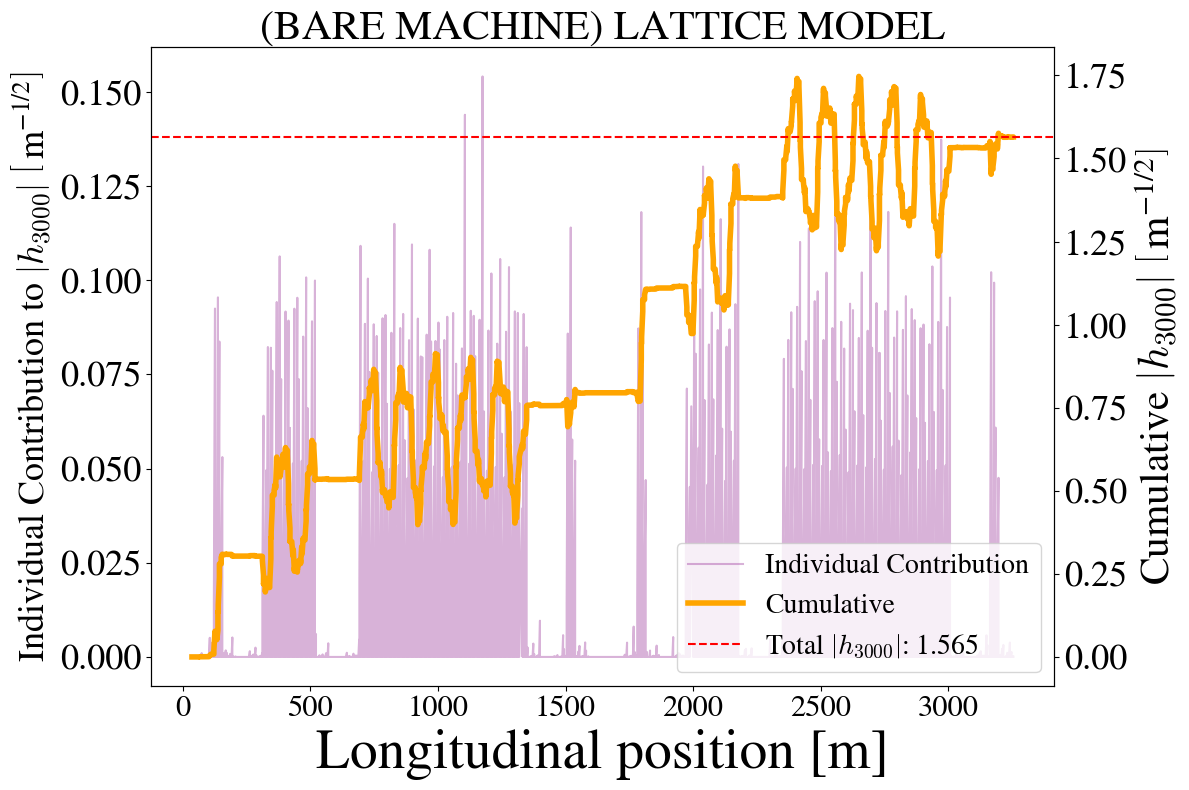
\includegraphics[width=0.88\columnwidth]{chapter4/h3000_bare.png}
    \caption{Distribution of the $h_{3000}$ term around the ring with individual contributions from each relevant element and the cumulative sum from an arbitrary starting point.}
    \label{fig:h3000bare}
\end{figure}

\begin{figure}[H]
    \centering
    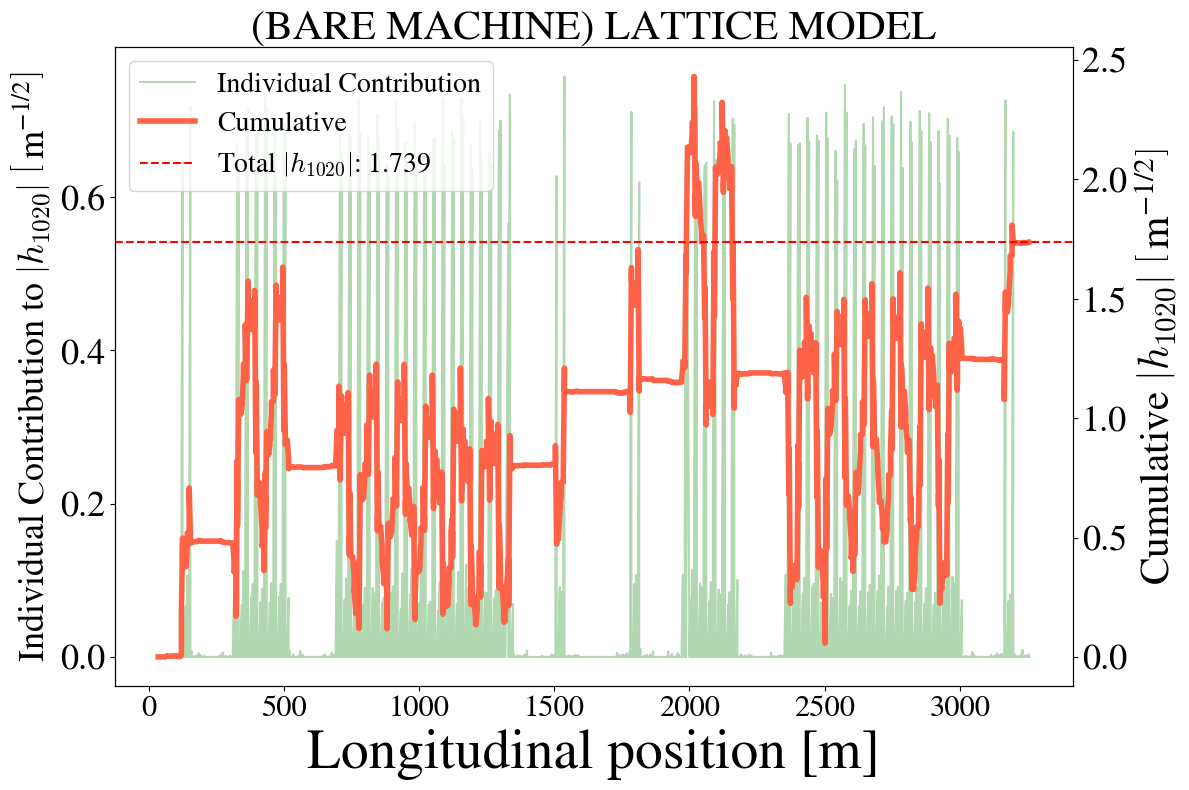
\includegraphics[width=0.88\columnwidth]{chapter4/h1020_bare.png}
    \caption{Distribution of the $h_{1020}$ term around the ring with individual contributions from each relevant element and the cumulative sum from an arbitrary starting point.}
    \label{fig:h1020bare}
\end{figure}

\section{\label{sec:rdtmeasure}Measurement of Third Order RDTs}

Calculating the theoretical RDTs from the lattice model is a matter of calculating the sums outlined in Table \ref{tab:rdts}. Nevertheless, the measurement of the third order RDTs requires following a long and involved recipe. This recipe is based on previous work from Refs. \cite{cernthesis2,bartolini}, but with a lot of original steps specifically developed for the Recycler Ring. In summary, these are the steps used in order to measure RDTs at the Recycler:
\begin{enumerate}
    \item Kick the beam with dipole kickers and save turn-by-turn BPM data for offline analysis.
    \item Go through data and estimate momentum coordinate with previously calculated transfer matrices from lattice model.
    \item Estimate Twiss parameters and normalized coordinates ($\hat{u}$,$\hat{p}_u$) at every BPM location.
    \item Create resonance basis $h_u^{\pm}$ (see Eq. \ref{eq:hbasis}).
    \item Get spectrum of resonance basis using NAFF (Numerical Analysis of Fundamental Frequencies) through the SUSSIX software \cite{sussix}.
    \item Identify resonance lines from the spectrum that correspond to the RDT of interest.
    \item Calculate the RDT at each BPM location from the equivalence relation of spectral lines and RDT expansion (see Eq. \ref{eq:hx-}). 
\end{enumerate}
The following subsections will explore in more detail the steps outlined in the previous list.

\subsection{Dipole Kick and BPM data}

The first step towards measuring RDTs is to kick (or ping) the beam in one or both transverse direction(s) in order to excite betatron oscillations. Betatron oscillations are the natural oscillations of particles around their equilibrium orbit in a circular accelerator. This kick is done with the help of horizontal and vertical dipole kickers. In particular, the devices used for this were the kicker devices with ACNET names R:K4XXX and R:KVXXX, horizontally and vertically, respectively. In principle, these are the Recycler abort kickers---devices used to send beam to the abort line in Recycler. Nevertheless, the high-voltage settings and timings of these pingers can be changed to give a small kick to the beam. A ping that is small enough not to steer the beam to the abort line, but large enough to excite betatron oscillations in one or both transverse directions. The beam was kicked exclusively in the horizontal direction in order to measure purely horizontal RDTs, e.g., $h_{3000}$, solely in the vertical direction for vertical RDTs, e.g., $h_{0030}$, or pinged in both directions for all of them, including coupling RDTs, e.g., $h_{1020}$ and $h_{2010}$.

Once the kickers are set correctly, the next step is to take BPM data. As mentioned in Sec. \ref{sec:diagnostic}, there are ACNET applications that allow to gather and save BPM data for offline analysis. The BPM data from all 208 BPMs (104 horizontal and 104 vertical) can be saved in one file. Figure \ref{fig:bpm_kick0} shows an instance of kicking the beam in the horizontal direction and recording beam centroid data for 2048 turns at an arbitrary BPM. The amount of turns recorded is also a customizable quantity. The ping shown in Fig. \ref{fig:bpm_kick0} happens early in the cycle, at around 50 turns. The next hundred of turns holds information about the betatron oscillations. This is the data used to extract the tunes $Q_u$ and RDTs of the machine.

\begin{figure}[H]
    \centering
    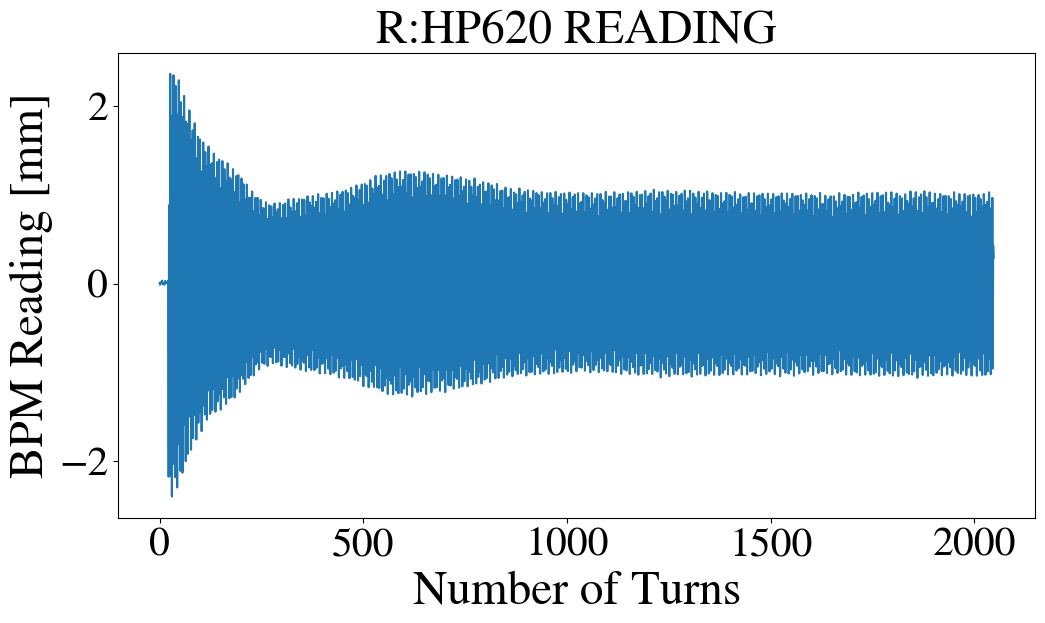
\includegraphics[width=\columnwidth]{chapter4/bpm_kick.png}
    \caption{BPM data of an arbitrary horizontal kick in the beam at horizontal BPM R:HP620.}
    \label{fig:bpm_kick0}
\end{figure}

The physics of a kicked beam is well explained in Refs. \cite{decoherence1,decoherence2}. Once the beam is pinged, the centroid response will oscillate at betatron tunes $Q_u$. The envelope of these oscillations will be dictated by nonlinearities and chromaticity of the machine. How fast this envelope decays is a measure of the decoherence of the beam. Decoherence of a particle beam in accelerator physics refers to the process by which a beam that initially has particles oscillating in phase—--meaning they have similar amplitudes and frequencies—--gradually becomes out of phase over time. This results in a spread in the particles' positions and momenta, leading to a more diffuse beam. This decoherence is caused by nonlinearities in the machine and the transverse chromaticities that will detune the beam out of coherence, as explained by Eqs. \ref{eq:detune} and \ref{eq:chrom}. Ultimately, this process will diffuse and maim the signal recorded by the BPMs. 

Therefore, when BPM data of kicked beam is taken, special care needs to be taken in order to sustain coherent oscillations. This is done by manipulating the chromaticities of the machine by means of specialized sextupoles. Table \ref{tab:rrparams} showed the nominal chromaticities at which the Recycler Ring operates. In general, for these RDT measurements, the vertical chromaticity was changed between the range of -7 and -3, in order to find sustained vertical oscillations. For the horizontal case, a chromaticity of -5 would be usually enough for 1 mm oscillations. The other system that affects decoherence are the transverse dampers. As per its name, these devices dampen out any oscillation in the beam. Therefore, they were turned off for these particular studies. Taking these factors into account, one could get consequential oscillations in both transverse planes, as a first step to measure Resonance Driving Terms.      

\subsection{Estimation of Momentum Coordinate}

At the most fundamental level, BPM data holds only information about the centroid position of the beam. Nevertheless, in a particle accelerator it is of interest to look at the whole phase space picture ($\hat{u},\hat{p}_u$)---including the momentum coordinate. Therefore, it is of relevance to explain how the momentum coordinate is calculated from the TbT position from every BPM. The approach used involves a model-based perspective. Therefore, the lattice model plays a crucial role in the momentum estimation.    

The approach to estimate the momentum coordinate involves solving a least-squares problem. This is the approach developed in Ref. \cite{yang}. The first step is to calculate the model's transfer matrices (linear approximation) from one fixed point in the accelerator to all the horizontal and vertical BPM locations---in total there should be 208 transfer matrices. For these studies, the fixed point chosen was the starting point of the turn count which is the location for the vertical BPM R:VP601. As an example, let the following paragraphs show how to calculate the horizontal phase space coordinates, including the relative momentum deviation $\delta$. In particular, the main objective is to calculate the $X_0$ matrix with dimensions $3\times2048$, which corresponds to the phase space coordinates $\left( \vec{x}_0, \vec{x}_0', \vec{\delta}_0 \right)$ at the location of R:VP601. The $X_0$ array will have the following definition:
\begin{equation}
    \label{eq:x0vec}
    X_0= 
    \begin{pmatrix}
        \vec{x_0} \\
        \vec{x}_0' \\
        \vec{\delta_0}
    \end{pmatrix} = 
    \begin{pmatrix}
        \left[ x_0(N=1), x_0(N=2), ...,x_0(N=2048) \right] \\
        \left[ x_0'(N=1), x_0'(N=2), ..., x_0'(N=2048) \right] \\
        \left[ \delta_0 (N=1), \delta_0 (N=2), ..., \delta_0 (N=2048) \right]
    \end{pmatrix},
\end{equation}  
and holds the information over the 2048 turns. The least squares problem is defined as the solution to the following system:
\begin{equation}
    \label{eq:lsq}
    A X_0 = B,
\end{equation}
where $A$ is the matrix made from the horizontal coefficients of the model's transfer matrices, and it reads: 
\begin{equation}
\label{eq:alsq}
    A =
    \begin{pmatrix}
    \left( M_{11} \qquad M_{12} \qquad M_{13} \right)_{BPM(i-10)} \\
    \vdots \\
    \left( M_{11} \qquad M_{12} \qquad M_{13} \right)_{BPM(i)}  \\
    \vdots \\
    \left( M_{11} \qquad M_{12} \qquad M_{13} \right)_{BPM(i+10)} 
    \end{pmatrix}.
\end{equation}
The notation $(...)_{BPM(j)}$ means that all the matrix coefficients inside the parenthesis are indexed by the BPM(j), and should be copied from that particular transfer matrix correlating the fixed point to BPM(j). For this case, the BPM(i) corresponds to the particular BPM location where the phase space coordinates $X_{BPM(i)}$ want to be calculated, after calculating $X_0$. It can be noted, that only the 10 upstream BPMs and 10 downstream BPMs of BPM(i) are included in this calculation. This number is easily customizable in this estimation, but should not be too large, i.e., no larger than 30 to preserve some sense of locality. 

The $B$ matrix is defined from the BPM observations, and its transpose is just the BPM responses stacked horizontally. This reads explicitly:
\begin{equation}
    \label{eq:balsq}
    B^T =
    \begin{pmatrix}
    \vdots & & \vdots & & \vdots \\
    \Bigl< x_{BPM(i-10)} \Bigr> & ... &  \Bigl< x_{BPM(i)} \Bigr> &  ... & \Bigl< x_{BPM(i+10)} \Bigr> \\
    \vdots & & \vdots & & \vdots \\
    \end{pmatrix}. 
\end{equation}
For Eq. \ref{eq:balsq}, the triangular bracket notation $\langle ... \rangle$ is used to specify that the BPM data inside the brackets has already been averaged out---the oscillations recorded in the BPM data is centered around 0. Again, in order to use least-squares approximation, this calculation should take the 10 BPMs upstream and the 10 BPMs downstream of the BPM(i), whose phase space coordinates are being calculated. 

The least-squares solution $\hat{X}_0$ to this problem is given by:
\begin{equation}
    \label{eq:x0hat}
    \hat{X}_0 = (A^T A)^{-1} A^T B.
\end{equation}
Once $\hat{X}_0$ is calculated from the data of 10 BPMs upstream and downstream of BPM(i). The phase space coordinates $\hat{X}_{BPM(i)}$ at BPM(i) can be calculated from:
\begin{equation}
    \label{eq:xbpmi}
    \hat{X}_{BPM(i)} = \begin{pmatrix}
        \vec{x} \\
        \vec{x}' \\
        \vec{\delta}
    \end{pmatrix}_{BPM(i)}=
    \begin{pmatrix}
        \left[ x(N=1),...,x(N=2048) \right] \\
        \left[ x'(N=1),..., x'(N=2048) \right] \\
        \left[ \delta (N=1),..., \delta (N=2048) \right]
    \end{pmatrix}
    = \left[ M_{11} \quad M_{12} \quad M_{13} \right]_{BPM(i)} \hat{X}_0.  
\end{equation}
The hat notation $\hat{X}$ is to symbolize that this is data estimated based on the least-squares solution to Eq. \ref{eq:x0hat}. 

Similar to the horizontal case, for the vertical case, the phase space coordinates at each BPM location can be estimated by first estimating the phase space coordinates $Y_0$ at an arbitrary location in the lattice---vertical BPM R:VP601 for this case. At this location, the $Y_0$ array will be defined as:
\begin{equation}
    \label{eq:y0vec}
    Y_0= 
    \begin{pmatrix}
        \vec{y_0} \\
        \vec{y}_0'
    \end{pmatrix} = 
    \begin{pmatrix}
        \left[ y_0(N=1), y_0(N=2), ...,y_0(N=2048) \right] \\
        \left[ y_0'(N=1), y_0'(N=2), ..., y_0'(N=2048) \right]
    \end{pmatrix}.
\end{equation} 
The least-squares estimate $\hat{Y}_0$ for the array in Eq. \ref{eq:y0vec} from the recorded BPM data will be given by:
\begin{equation}
    \label{eq:y0hat}
    \hat{Y}_0 = (A_y^T A_y)^{-1} A_y^T B_y,
\end{equation}
where similar to the horizontal case, the matrix $A_y$ is defined by:
\begin{equation}
    \label{eq:alsqy}
        A_y =
        \begin{pmatrix}
        \left( M_{21} \qquad M_{22} \right)_{BPM(i-10)} \\
        \vdots \\
        \left( M_{21} \qquad M_{22} \right)_{BPM(i)}  \\
        \vdots \\
        \left( M_{21} \qquad M_{22} \right)_{BPM(i+10)} 
        \end{pmatrix},
\end{equation}
and $B_y$ is defined by
\begin{equation}
    \label{eq:balsqy}
    B_y^T =
    \begin{pmatrix}
    \vdots & & \vdots & & \vdots \\
    \Bigl< y_{BPM(i-10)} \Bigr> & ... &  \Bigl< y_{BPM(i)} \Bigr> &  ... & \Bigl< y_{BPM(i+10)} \Bigr> \\
    \vdots & & \vdots & & \vdots \\
    \end{pmatrix}. 
\end{equation}
Once, $\hat{Y}_0$ is calculated, it can be transferred to the location of BPM(i) by means of the transfer matrices. This is the way of calculating $\hat{Y}_{BPM(i)}$, which reads
\begin{equation}
    \label{eq:ybpmi}
    \hat{Y}_{BPM(i)} = \begin{pmatrix}
        \vec{y} \\
        \vec{y}' \\
    \end{pmatrix}_{BPM(i)}=
    \begin{pmatrix}
        \left[ y(N=1),...,y(N=2048) \right] \\
        \left[ y'(N=1),..., y'(N=2048) \right] 
    \end{pmatrix}
    = \left[ M_{21} \quad M_{22} \right]_{BPM(i)} \hat{Y}_0.  
\end{equation}

It is worth pointing out that for the vertical case, the appropriate elements of the transfer matrices are picked out, i.e., $M_{21}$ and $M_{22}$ instead of the horizontal coefficients $M_{11}$, $M_{12}$ and $M_{13}$. The other thing to note is that for the vertical case any momentum dependence is dropped given that the vertical dispersion is negligible in the Recycler Ring, as shown in Fig. \ref{fig:rrdisps}. The previous procedure of calculating $\hat{U}_{BPM(i)}$ is done and saved for each of the 104 horizontal and 104 vertical BPMs---$\hat{X}_{BPM(i)}$ or $\hat{Y}_{BPM(i)}$, accordingly. Figure \ref{fig:momentum} shows an application of this momentum reconstruction technique for a horizontal BPM R:HP620 and its vertical neighbor R:VP621. 

With model-based approaches, it is important to be confident that the model is as close to the real accelerator as possible. The beta-beating is a measure of how well the beta functions of the model describe the beta functions from the real-world accelerator. In particular, M. Xiao has showed that the beta-beating along the Recycler is below 10\% \cite{rr3}---an acceptable quantity for modern accelerators. Therefore, this proves that the model used is reliable up to some significance level. The beta-beating quantity is ultimately limited by how truly linear the accelerator is and any ripple noise from the power supplies feeding the quadrupole and dipoles.

\begin{figure}[H]
    \centering
    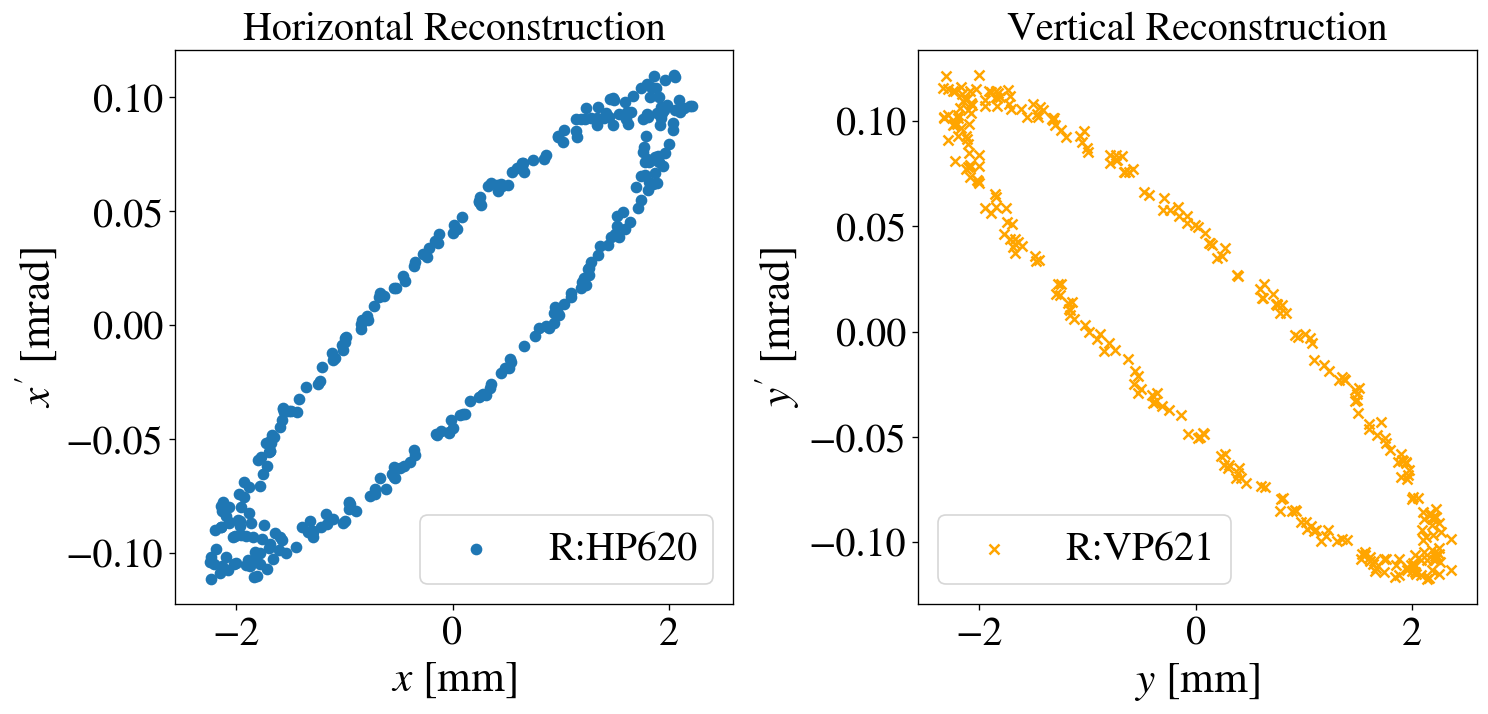
\includegraphics[width=\columnwidth]{chapter4/momentum.png}
    \caption{Phase space coordinates reconstruction for two neighboring BPMs---one horizontal R:HP620 and one vertical R:VP621---windowed for 300 turns.}
    \label{fig:momentum}
\end{figure}

\subsection{Twiss Parameters and Normalized Phase Space}

The next step to measure RDTs, once the phase space coordinates have been reconstructed for every BPM, is to build the normal phase space coordinates ($\hat{u}$,$\hat{p}_u$). This is done by using Eqs. \ref{eq:ellipse} and \ref{eq:floquet}, and the information provided in Fig. \ref{fig:ellipses}. In order to build the normalized phase space, first the Twiss parameters have to be estimated. This is done by performing a least-squares fit in order to estimate the ellipse parameters of reconstructed phase space, such as the one shown in Fig. \ref{fig:momentum}. Therefore, an ellipse is being fit to the data, and after that, the Twiss parameters are retrieved from the fit, including the centroid action $2 \pi \langle J_u \rangle =\varepsilon_x $ (see Eq. \ref{eq:ellipse}). 

Figure \ref{fig:ellipse} shows an example of this procedure. The left plot shows reconstructed phase space data with the best ellipse fit. The parameters indicated on the inset provide detailed characteristics of this particular fit: (a) $\beta_x$ (beta function) describes the spatial spread of the beam, (b) $\alpha_x$ (alpha function) relates to the angle the beam particles make with the reference orbit, and it is a measure of the beam divergence, and (c) $\varepsilon_x$ (centroid emittance) quantifies the area of the phase space that the beam centroid occupies. In particular, the centroid action can be calculated from $2 \pi \langle J_u \rangle =\varepsilon_x $.

The right plot of Fig. \ref{fig:ellipse} shows the reconstructed normalized phase space using the Twiss parameters, as estimated from the ellipse fit. This normalization process involves scaling by the square root of the Twiss parameter $\beta_u$ at that particular location, in accordance to Floquet's transformation as defined in Eq. \ref{eq:floquet}. This procedure is done for the reconstructed data of every BPM, and, finally ($\hat{u}$,$\hat{p}_u$) is recorded.  

\begin{figure}[H]
    \centering
    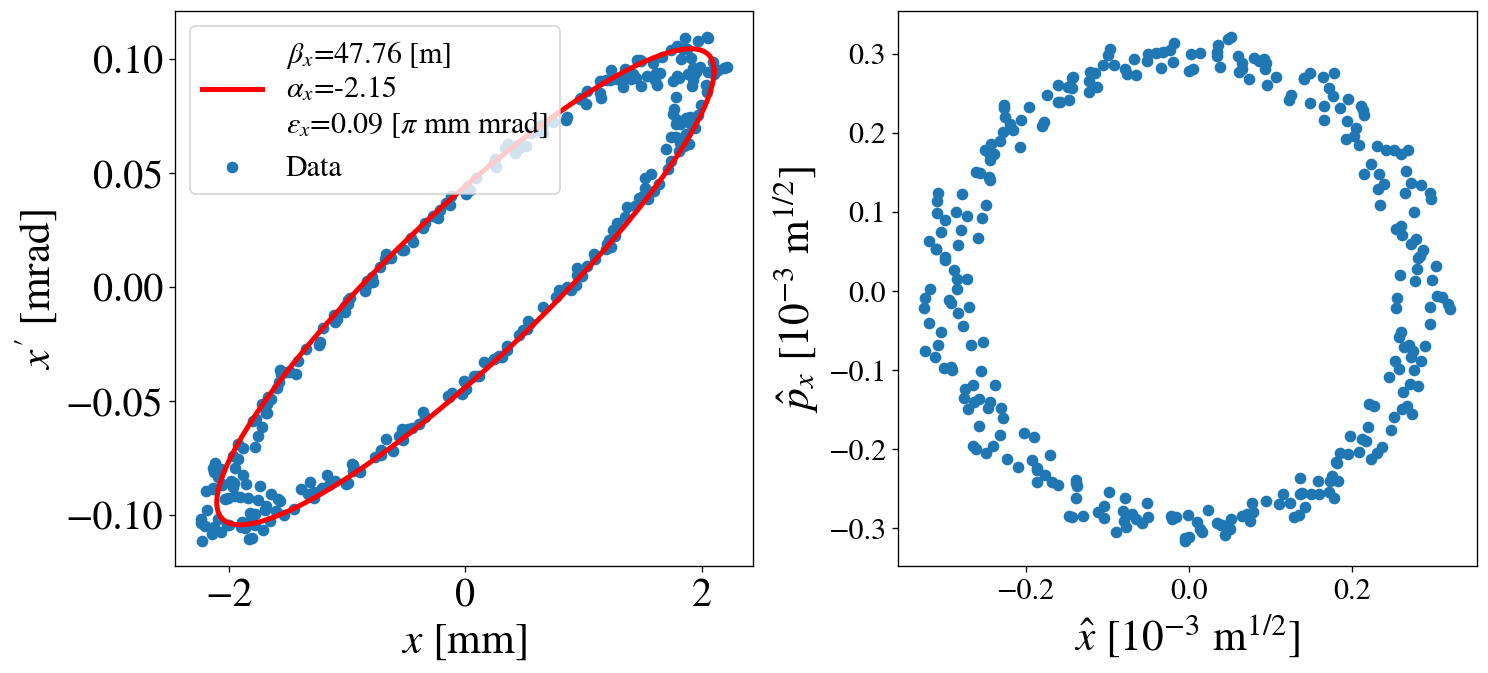
\includegraphics[width=\columnwidth]{chapter4/ellipse_data.png}
    \caption{Reconstructed phase space data with the best ellipse fit (left plot). The right plot shows the reconstructed normalized phase space from using Eq. \ref{eq:floquet} with the Twiss parameters, as estimated from the ellipse fit. This data corresponds to the horizontal data shown in Fig. \ref{fig:momentum} for the R:HP620 BPM.}
    \label{fig:ellipse}
\end{figure}

\subsection{Resonance Basis and Spectral Decomposition}

Once the normalized phase space coordinates are reconstructed for every BPM, the next step is to build the resonance basis $h_u^{\pm}(N)$, as defined in Eq. \ref{eq:hbasis}, i.e., $h_u^{\pm}=\hat{u}\pm \hat{p}_u$. This resonance basis is a function of the number of the turns $N$ that have elapsed. As shown in Eq. \ref{eq:hx-}, this quantity can have a spectral decomposition as a Fourier series. In general, this spectral decomposition in the horizontal dimension reads: 
\begin{equation}
    \label{eq:hxspect}
    h_x^{-}(N)= \hat{x} \pm \hat{p}_x = \sum_{jklm}HSL_{jklm}e^{2\pi i N \left[ \left( 1-j+k\right)Q_x+\left( m-l \right)Q_y\right]},
\end{equation}
and in the vertical dimension:
\begin{equation}
    \label{eq:hyspect}
    h_y^{-}(N)= \hat{y} \pm \hat{p}_y = \sum_{jklm}VSL_{jklm}e^{2\pi i N \left[ \left( k-j\right)Q_x+\left(1-l+m \right)Q_y\right]}.
\end{equation}
These sums run over the $(j,k,l,m)$ indices. In principle, they run all the way to infinity, but can be truncated. The $HSL_{jklm}$ term corresponds to the complex amplitude defining the horizontal spectral line at frequency location $(1-j+k)Q_x+(m-l)Q_y$. The $VSL_{jklm}$ term corresponds to the complex amplitude defining the vertical spectral line at location $(k-j)Q_x+(1-l+m)Q_y$. And, as always, $Q_u$ corresponds to the betatron tunes. These definitions help to understand the experimental data in order to measure RDTs.

Nevertheless, from the theoretical point of view, the spectral decomposition can be calculated with the Lie algebra gymnastics shown in Sec. \ref{sec:rdts}. These spectral decompositions read for the horizontal plane:
\begin{multline}
    \label{eq:hxpsi2}
    h_x^{-}(N)=\sqrt{2I_x}e^{i\left( 2 \pi Q_x N+\psi_{x_0}\right)} \\
    -2i \sum_{jklm} j f_{jklm} \left( 2I_x \right)^{\frac{j+k-1}{2}}\left( 2I_y \right)^{\frac{l+m}{2}}
    e^{i \left[ \left( 1-j+k\right)\left( 2 \pi Q_x N + \psi_{x_0} \right) +\left( m-l\right)\left( 2 \pi Q_y N + \psi_{y_0} \right)\right]},
\end{multline}
and for the vertical case:
\begin{multline}
    \label{eq:hypsi2}
    h_y^{-}(N)=\sqrt{2I_y}e^{i\left( 2 \pi Q_y N+\psi_{y_0}\right)} \\
    -2i \sum_{jklm} l f_{jklm} \left( 2I_x \right)^{\frac{j+k}{2}}\left( 2I_y \right)^{\frac{l+m-1}{2}}
    e^{i \left[ \left( k-j\right)\left( 2 \pi Q_x N + \psi_{x_0} \right) +\left( 1-l+m\right)\left( 2 \pi Q_y N + \psi_{y_0} \right)\right]}.
\end{multline}
The RDT calculation exploits the equivalence between Eqs. \ref{eq:hxspect} and \ref{eq:hyspect} to Eqs. \ref{eq:hxpsi2} and \ref{eq:hypsi2}. Therefore, the generating function coefficients ($f_{jklm}$) can be related to the horizontal and spectral line coefficients ($HSL_{jklm}$ and $VSL_{jklm}$). Ultimately, the $f_{jklm}$ terms can be related to Resonance Driving Terms $h_{jklm}$ through Eq. \ref{eq:handf}.

A quick comparison between Eqs. \ref{eq:hxspect} and \ref{eq:hxpsi2} allows to build an equivalence table between the generating function coefficients (GFCs) and the spectral lines. Table \ref{tab:sls} is the result of this. This table can be originally found in Refs. \cite{sussix,bartolini}. Table \ref{tab:sls} shows how to calculate the GFCs from its corresponding spectral line. In particular, the amplitude and phase of a spectral line will be given by $|USL_{jklm}|$ and $\arg(USL_{jklm})$, while its location in its corresponding frequency space will be given by $Q(USL_{jklm})$. It is worth pointing out that in this notation $U$ can be either the horizontal or vertical plane.

\begin{table}[H]
    \centering
    \caption{Equivalence table between the generating function coefficients and the spectral lines.}
    \label{tab:sls}
    \begin{tabular}{c|c|c|}
    \cline{2-3}
     & \textbf{\begin{tabular}[c]{@{}c@{}}Generating Function\\ Coefficient\end{tabular}} & \textbf{Spectral Line} \\ \hline
    \multicolumn{1}{|c|}{} &  &  \\
    \multicolumn{1}{|c|}{\textbf{Amplitude}} & $\left| f_{jklm}\right|$ & $\left| HSL_{jklm} \right|=2 \; j \; \left( 2I_x \right)^{\frac{j+k-1}{2}}\left( 2I_y \right)^{\frac{l+m}{2}} \left| f_{jklm}\right|$ \\
    \multicolumn{1}{|c|}{} &  &  \\
    \multicolumn{1}{|c|}{} &  & $\left| VSL_{jklm} \right|=2 \; l \; \left( 2I_x \right)^{\frac{j+k}{2}}\left( 2I_y \right)^{\frac{l+m-1}{2}} \left| f_{jklm}\right|$ \\
    \multicolumn{1}{|c|}{} &  &  \\ \hline
    \multicolumn{1}{|c|}{\textbf{}} &  &  \\
    \multicolumn{1}{|c|}{\textbf{Phase}} & $\phi_{jklm}= \arg{(f_{jklm})}$ & $\arg{(HSL_{jklm})} = \phi_{jklm}+\psi_{x_0}-\frac{\pi}{2}$ \\
    \multicolumn{1}{|c|}{} &  &  \\
    \multicolumn{1}{|c|}{} &  & $\arg{(VSL_{jklm})} = \phi_{jklm}+\psi_{y_0}-\frac{\pi}{2}$ \\
    \multicolumn{1}{|c|}{\textbf{}} &  &  \\ \hline
    \multicolumn{1}{|c|}{\textbf{}} &  &  \\
    \multicolumn{1}{|c|}{\textbf{Spectral}} & N/A & $Q\left( HSL_{jklm} \right) = (1-j+k)Q_x+(m-l)Q_y$ \\
    \multicolumn{1}{|c|}{\textbf{Harmonic}} &  &  \\
    \multicolumn{1}{|l|}{} & \multicolumn{1}{l|}{} & $Q\left( VSL_{jklm} \right) = (k-j)Q_x+(1-l+m)Q_y$ \\
    \multicolumn{1}{|l|}{} & \multicolumn{1}{l|}{} & \multicolumn{1}{l|}{} \\ \hline
    \end{tabular}
\end{table}

\subsection{Resonance Basis Spectrum}

As mentioned in the last section, the spectral lines of the resonance basis hold enough information in order to reconstruct the generating function coefficients (GFCs) and, ultimately, the resonance driving terms (RDTs). Therefore, it is of interest to have a program that reconstructs the spectral lines from $h_u^{\pm}(N)$ data. This is exactly what SUSSIX \cite{sussix} does. This is a software developed at CERN, and it utilizes the Numerical Analysis of Fundamental Frequencies (NAFF) algorithm to identify and calculate the resonance lines up to an arbitrary order. SUSSIX can calculate spectral lines either for the horizontal, the vertical plane, or both planes.   

Figure \ref{fig:hxspect1} shows an example of spectrum data calculated using SUSSIX. The horizontal axis represents the frequency (or tune) of the spectral lines, while the vertical axis shows the amplitude of the lines, i.e., $|HSL_{jklm}|$. All the lines that show up in Fig. \ref{fig:hxspect1} represent the harmonics present in $h_x^{-}(N)$. The largest peak corresponds to the horizontal tune $Q_x$. In this case, the second-largest tune corresponds to the vertical tune $Q_y$, indicating some residual coupling. The lines $HSL_{2010}$, $HSL_{3000}$ and $HSL_{1020}$ are also marked with their location at the plot. These are the lines from which the relevant GFCs and RDTs are calculated from. Other unmarked spectral lines show up illustrating how there might be higher order harmonics and RDTs present in the oscillations. Specially, it is worth highlighting, how several RDTs can feed to the line located at $Q_x=0$. Figure \ref{fig:hyspect1} shows this exercise done but for the vertical resonance basis $h_y^{-}(N)$. In this case, the largest peak corresponds to the vertical tune $Q_y$, while the second-largest one corresponds to the horizontal tune $Q_x$. The lines $VSL_{2010}$, $VSL_{3000}$ and $VSL_{1020}$ also show up, but at different locations than their horizontal counterparts, as expected. The amplitudes of these spectral lines are at least three orders of magnitude less, than the main harmonic of the oscillations.  

\begin{figure}[H]
    \centering
    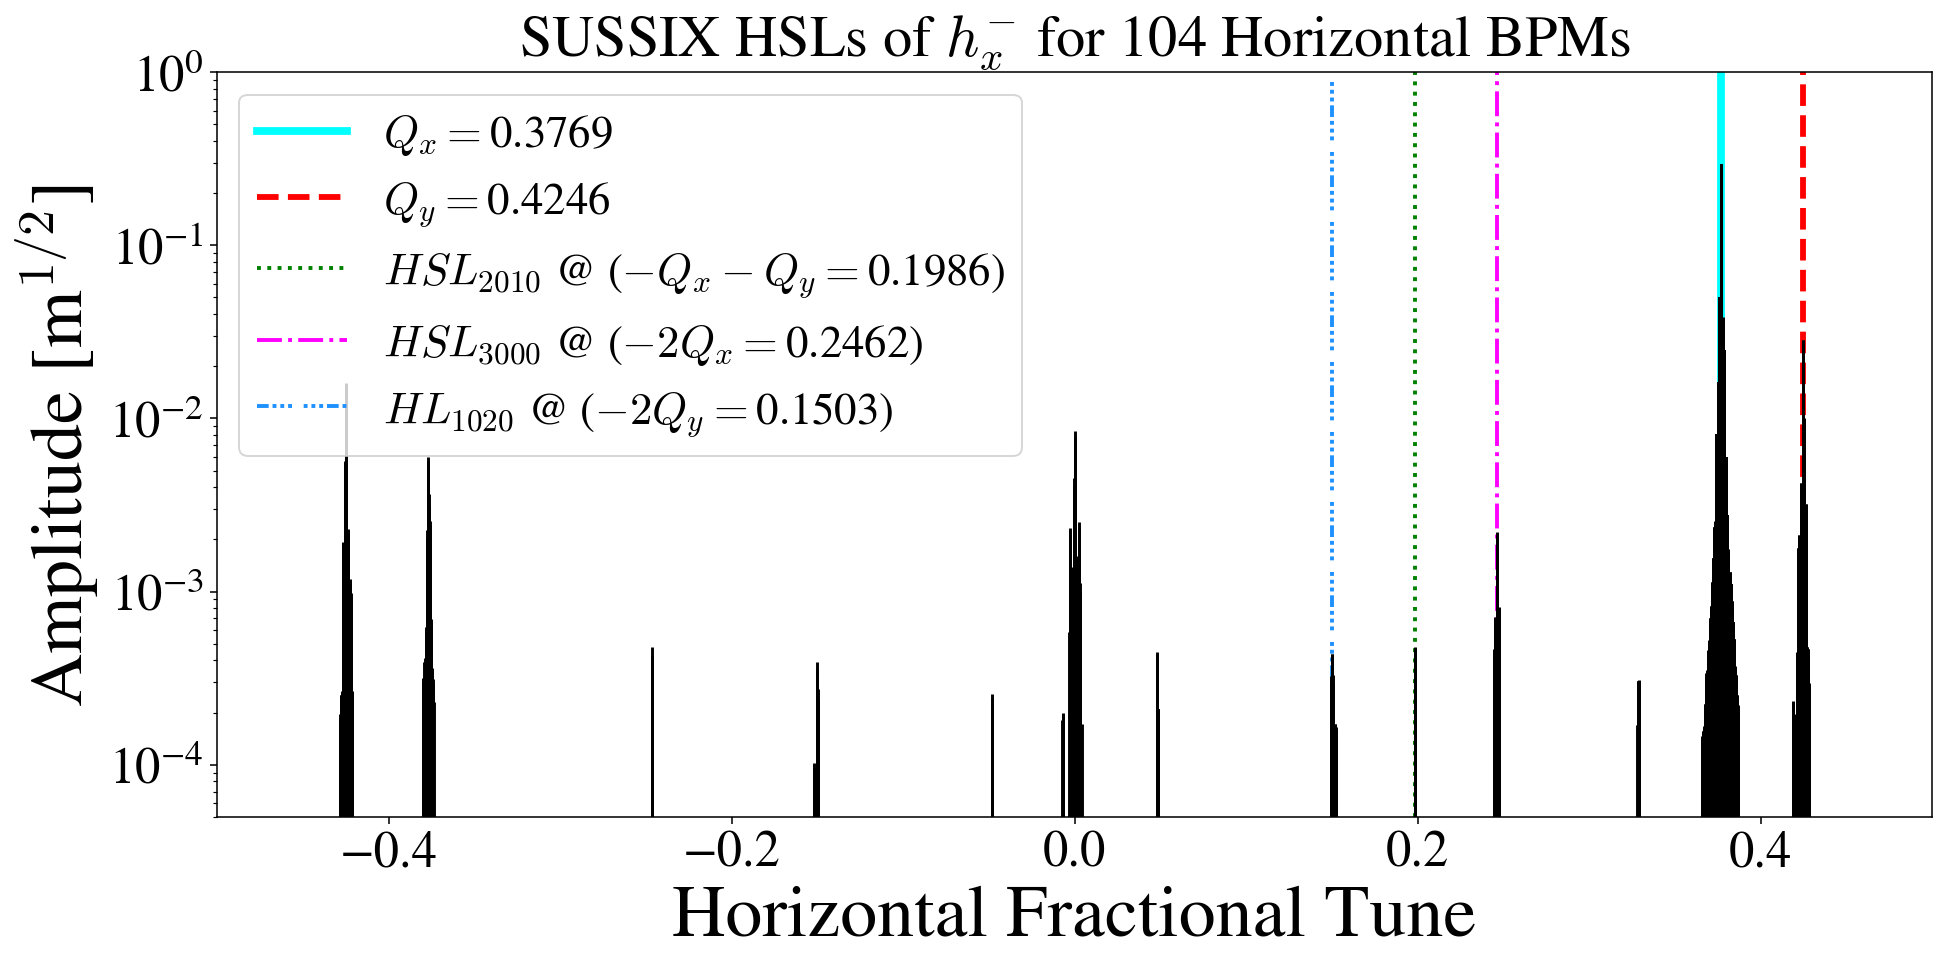
\includegraphics[width=\columnwidth]{chapter4/hxspect.png}
    \caption{Spectral lines of $h_x^{-}$ calculated with SUSSIX \cite{sussix}. The $h_x^{-}$ signal was reconstructed for the 104 Horizontal BPMs. The spectrum for all BPMs is superimposed in this plot.}
    \label{fig:hxspect1}
\end{figure}

\begin{figure}[H]
    \centering
    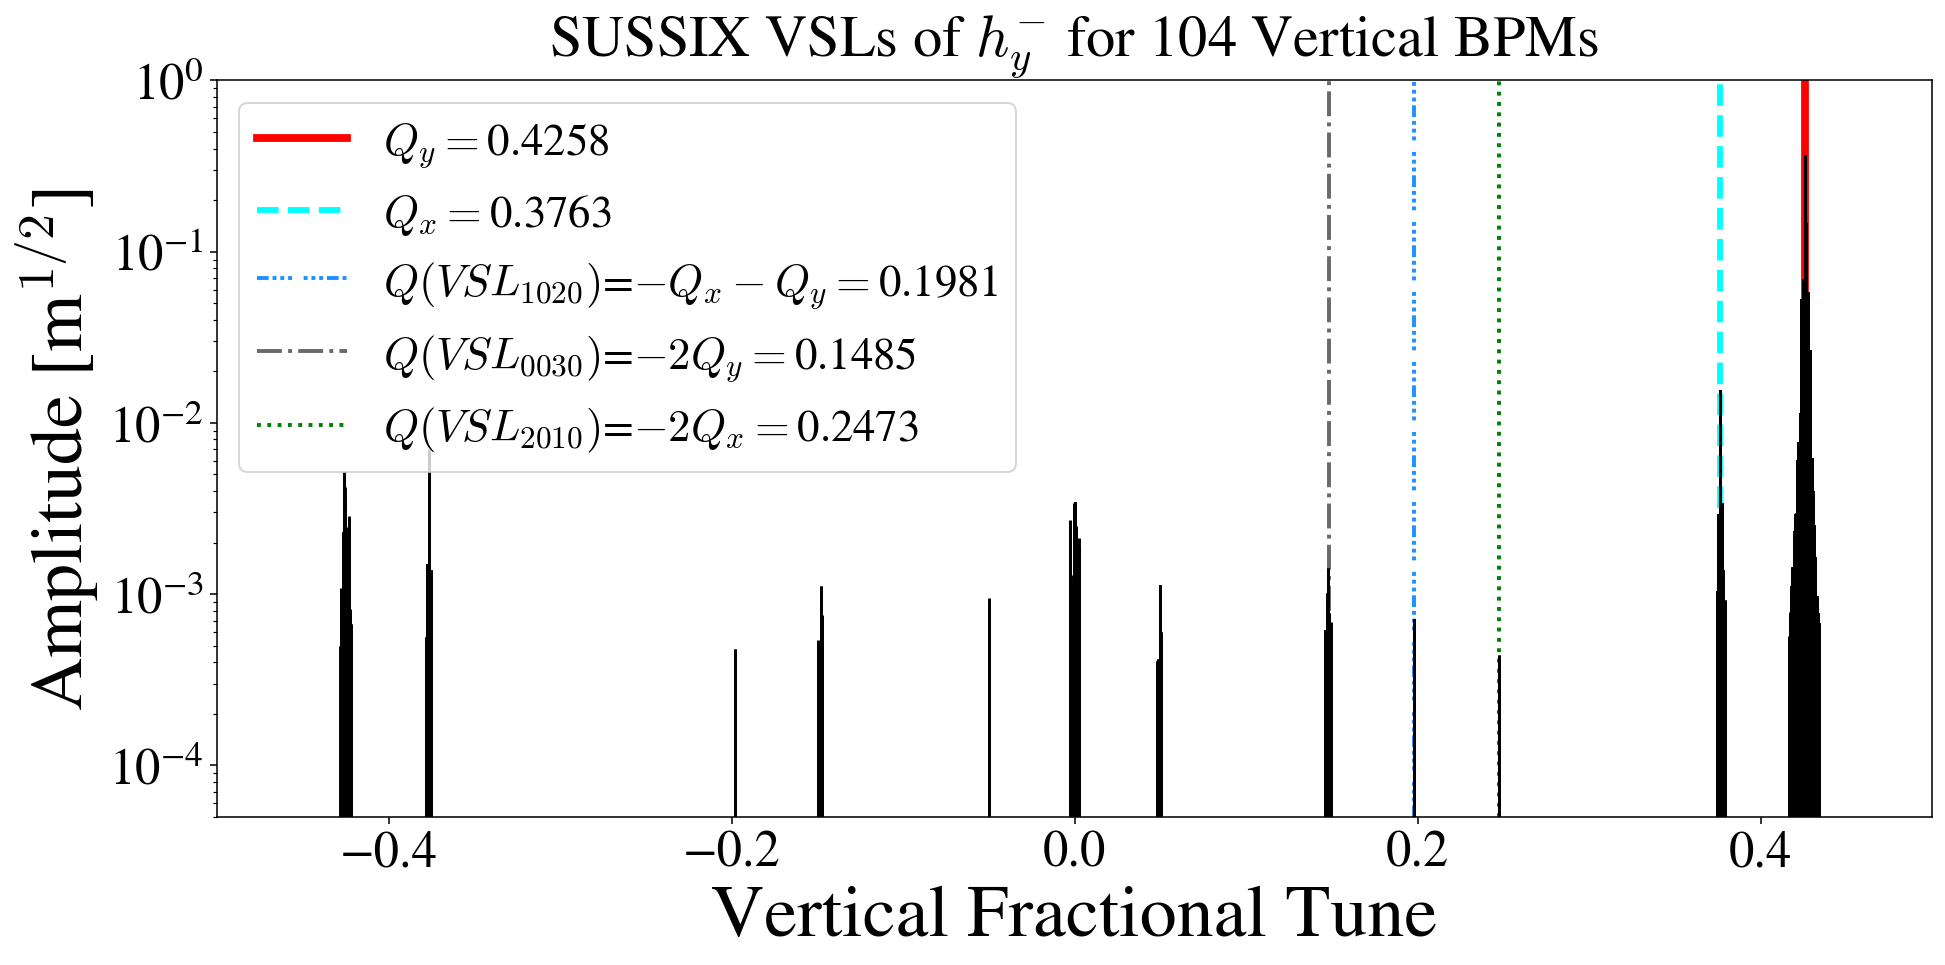
\includegraphics[width=\columnwidth]{chapter4/hyspect.png}
    \caption{Spectral lines of $h_y^{-}$ calculated with SUSSIX \cite{sussix}. The $h_y^{-}$ signal was reconstructed for the 104 Vertical BPMs. The spectrum for all BPMs is superimposed in this plot.}
    \label{fig:hyspect1}
\end{figure}

\subsection{Spectral Lines and RDT calculation}

The spectral lines $HSL_{3000}$, $HSL_{2010}$, and $HSL_{1020}$ identified in Fig. \ref{fig:hxspect1} are the necessary lines to calculate the $h_{3000}$, $h_{2010}$ and $h_{1020}$ RDTs. In combination with the $VSL_{0030}$ spectral line and its corresponding $h_{0030}$ RDT, these are all the spectral lines needed to calculate the RDTs for each resonance line shown in Fig. \ref{fig:rrtd} and specified in Table \ref{tab:rdtlines}. Table \ref{tab:rdts2} shows the explicit expressions for each resonance line RDT as a function of its GFC. In essence, once the $f_{jklm}$ is calculated using the expressions in Table \ref{tab:sls}, the RDT is just one multiplication away.

\begin{table}[H]
    \centering
    \caption{Corresponding RDTs from GFCs for each resonance line.}
    \label{tab:rdts2}
    \begin{tabular}{cc}
    \toprule
    \textbf{Resonance Line} & \textbf{RDT} \\ \hline
     &  \\
    $3Q_x=76$ & $h_{3000}= f_{3000}\left( 1-e^{6\pi i  Q_x  } \right)$ \\
     &  \\
    $Q_x+2Q_y=74$ & $h_{1020}=f_{1020} \left( 1-e^{2\pi i \left[Q_x + 2 Q_y \right] }\right) $ \\
     &  \\
    $3Q_y=73$ & $h_{0030}= f_{0030}\left( 1-e^{6\pi i  Q_y  } \right)$ \\
     &  \\
    $2Q_x+Q_y=75$ & $h_{2010}=f_{2010} \left( 1-e^{2\pi i \left[2Q_x + Q_y \right] }\right) $ \\
     &  \\ \hline
    \end{tabular}
\end{table}

% \begin{table}[H]
%     \centering
%     \caption{Corresponding RDTs from GFCs and location of spectral lines for each resonance line.}
%     \label{tab:rdts_sls}
%     \begin{tabular}{cccccc}
%     \textbf{Resonance Line} & \textbf{RDT} & \textbf{$HSL_{jklm}$} & \textbf{$Q_(HSL_{jklm})$} & \textbf{$VSL_{jklm}$} & \textbf{$Q_(VSL_{jklm})$} \\ \hline
%      &  &  &  &  &  \\
%     $3Q_x=76$ & $h_{3000}= f_{3000}\left( 1-e^{6\pi i  Q_x  } \right)$ & $HSL_{3000}$ & $-2Q_x$ & - & - \\
%      &  &  &  &  &  \\
%     $Q_x+2Q_y=74$ & $h_{1020}=f_{1020} \left( 1-e^{2\pi i \left[Q_x + 2 Q_y \right] }\right) $ & $HSL_{1020}$ & $-2Q_y$ & $VSL_{1020}$ & $-Q_x-Q_y$ \\
%      &  &  &  &  &  \\
%     $3Q_y=73$ & $h_{0030}= f_{0030}\left( 1-e^{6\pi i  Q_y  } \right)$ & - & - & $VSL_{0030}$ & $-2Q_y$ \\
%      &  &  &  &  &  \\
%     $2Q_x+Q_y=75$ & $h_{2010}=f_{2010} \left( 1-e^{2\pi i \left[2Q_x + Q_y \right] }\right) $ & $HSL_{2010}$ & $-Q_x-Q_y$ & $VSL_{2010}$ & $-2Q_x$ \\
%      &  &  &  &  &  \\ \hline
%     \end{tabular}
%     \end{table}

\subsection{Third Order RDTs at every BPM location}

Once the data from spectral lines is transformed to GFCs $f_{jklm}$, it is just a matter of using the expressions in Table \ref{tab:rdts2} to calculate the RDTs $h_{jklm}$. Figure \ref{fig:h3000_620} shows several measurements of the $h_{3000}$ term for the Recycler Ring from one particular BPM, i.e., R:HP620. This is a polar plot to indicate the amplitude and phase of this complex quantity. The left plot displays a set of 36 vectors representing individual measurements of the $h_{3000}$ term at a specific Beam Position Monitor (BPM) located at R:HP620. From this plot, one can see that there is some spread in the data from each measurement. This is due to changes in the beam coming from Booster for every injection and due to noise in BPM data. The right plot shows the average vector of the measurements, with its spread indicated by the shaded area. This spread signifies the variance in the data from measurement to measurement. 

\begin{figure}[H]
    \centering
    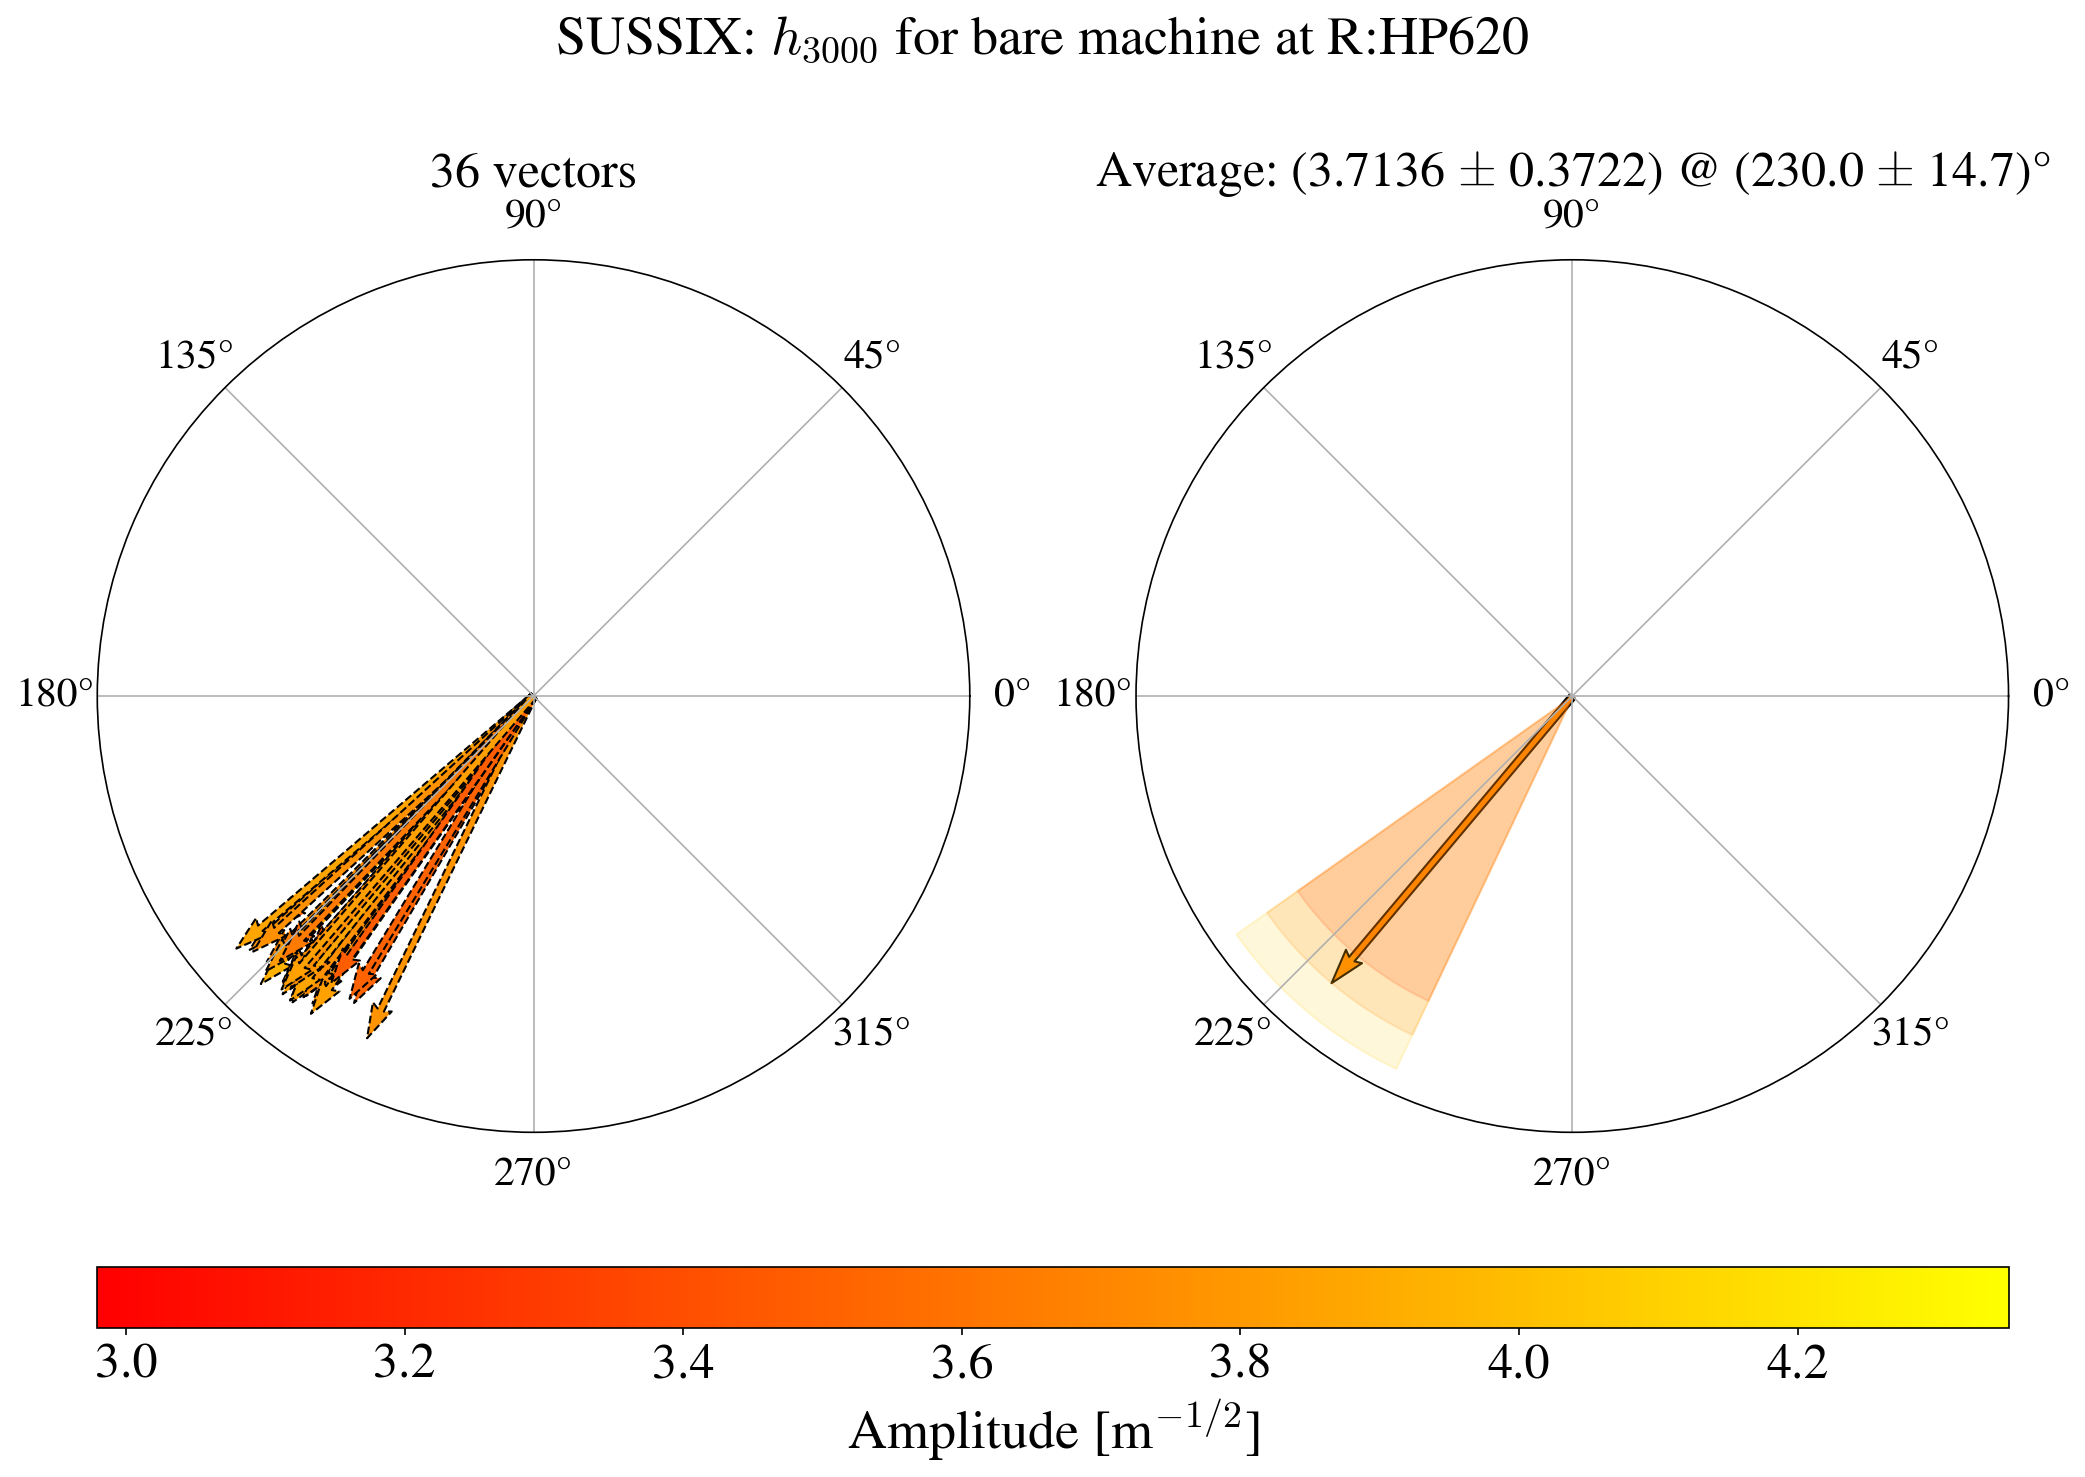
\includegraphics[width=\columnwidth]{chapter4/h3000_RHP620.png}
    \caption{Polar plot for the measurement of $h_{3000}$ for 36 measurements at horizontal BPM R:HP620.}
    \label{fig:h3000_620}
\end{figure}

Measurements such as the one presented for Fig. \ref{fig:h3000_620} are done for every BPM. In the case of the $h_{3000}$, the 104 horizontal BPMs are used. For the case of the $h_{0030}$ term, the 104 vertical BPMs are used. Figure \ref{fig:h3000_bpms} shows a plot of the amplitude of the measured $h_{3000}$ as a function of the BPM used. Each label (e.g., R:HP100, R:HP106,..., R:HP638) corresponds to a different BPM in the accelerator. The labels are ordered according to their physical positions along the Recycler Ring. Each point represents the amplitude of $h_{3000}$ measured at the corresponding BPM. The error bars on each data point indicate the uncertainty in the measurement, coming from the statistical variance as shown in Fig. \ref{fig:h3000_620}. The shaded background of Fig. \ref{fig:h3000_bpms} serves to visually emphasize the spread and distribution of the data points around the average. While there is a global spread, the local variations of $h_{3000}$ from BPM to BPM correspond to the amount of sextupole between them. Nevertheless, the large discontinuity at the 600 region---before R:HP602---comes from the momentum-estimation method which calculates the coordinates at R:VP601. Following all the previous steps in this recipe will allow to measure the RDTs at the Recycler Ring.

\begin{figure}[H]
    \centering
    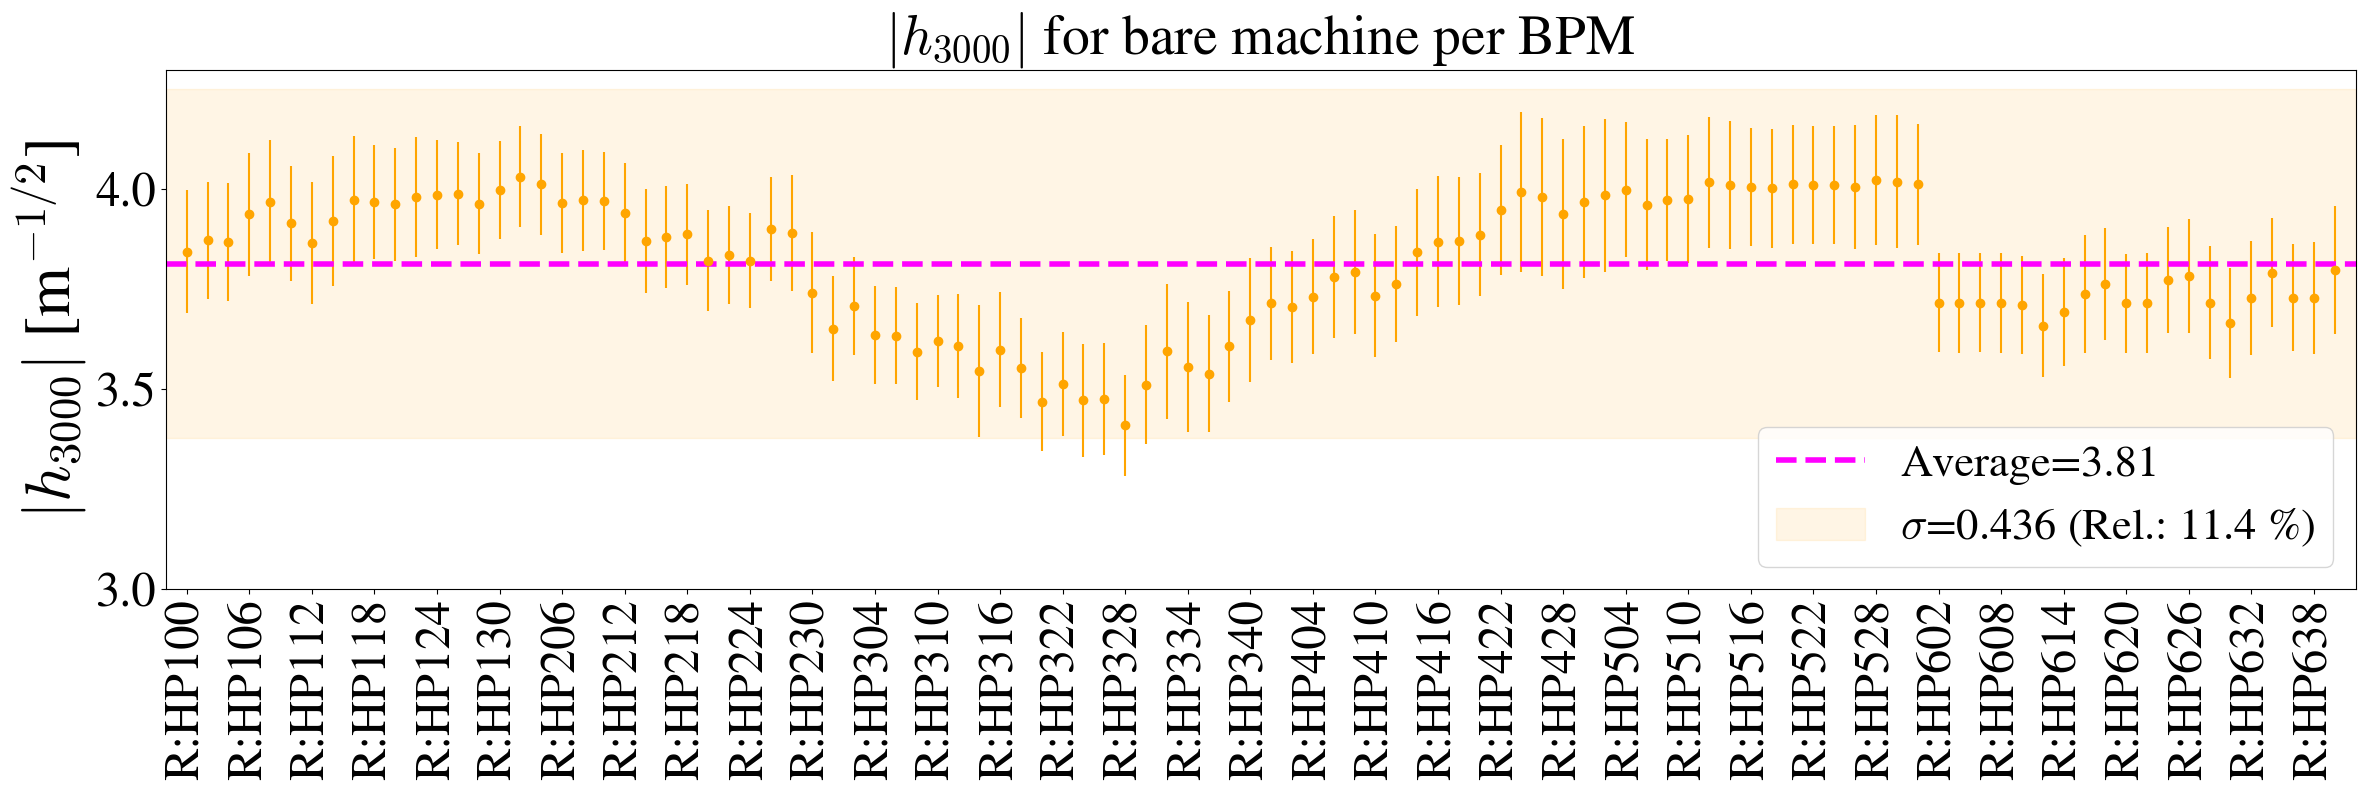
\includegraphics[width=\columnwidth]{chapter4/h3000_bpms.png}
    \caption{Measurements of $h_{3000}$ at all horizontal BPMs around the ring. The average (dashed line) corresponds to the average $h_{3000}$ from all the measurements.}
    \label{fig:h3000_bpms}
\end{figure}

\section{Compensation of RDTs}

\subsection{Theoretical Approach from Lattice Model}

Once there is a way to measure and/or calculate RDTs, the next step is to find a way to cancel out the RDTs. As mentioned in Sec. \ref{sec:css}, there are 4 normal sextupoles and 4 skew sextupoles that have been installed previously for this particular purpose. They have also been included in the lattice model. This section focuses on how to cancel out the RDTs from a lattice model perspective---just from theoretical considerations. The RDTs calculated from the lattice model as shown in Sec. \ref{sec:rdtslattice}.

The first step is to understand how to cancel out a single RDT---a single resonance line. For example, in order to compensate the $3Q_x$ line, the $h_{3000}$ would need to be cancelled. In order to cancel this term, the appropriate $K_2$ coefficients need to be set to the sextupoles. In practice, this is equivalent to setting the appropriate currents in the sextupoles. The appropriate $K_2$ coefficients are calculated from the following equation:
\begin{equation}
    \begin{bmatrix}
        -|h_{3000}| \cos \psi_{3000} \\
        -|h_{3000}| \sin \psi_{3000} \\
        0 \\
        0 \\
        \end{bmatrix}_{(Bare)}
         =
        \boldsymbol{M}
        \begin{bmatrix}
        K_2^{(sc220)} \\
        K_2^{(sc222)}\\
        K_2^{(sc319)} \\
        K_2^{(sc321)}\\
        \end{bmatrix},
        \label{eq:model1}
\end{equation}
where the $h_{3000}$ RDT is a complex quantity with a real and imaginary part, i.e., $h_{3000}= \left| h_{3000}\right|e^{i \psi_{3000}} = |h_{3000}| \cos \psi_{3000} + i |h_{3000}| \sin \psi_{3000}$. The $\boldsymbol{M}$ term corresponds to the RDT response matrix. And finally, the $K_2^{(i)}$ corresponds to the coefficient in the $i$-th compensation sextupole. The response matrix for compensating only $3Q_x$ and arbitrarily setting two sextupole currents to the negative of each other reads:
\begin{equation}
    \boldsymbol{M} = 
\begin{bmatrix}

M_{11} && M_{12} && M_{13} && M_{14}  \\ 

M_{21} && M_{22} && M_{23} && M_{24} \\ 

1 && 1 && 0 && 0 \\ 

0 && 0 && 1 && 1 \\

\end{bmatrix},
\label{eq:rm1}
\end{equation}
where the theoretical matrix coefficients are calculated from the derivatives of the expressions in Table \ref{tab:rdts} with respect to $K_2^{(i)}$, and they read: 
\begin{equation}
    M_{11}=\frac{1}{48} l_{sc} \: \beta^{3/2}_{x(sc220)} \: \cos 3\phi_{x(sc220)},
    \label{eq:M11}
\end{equation}
\begin{equation}
    M_{12}=\frac{1}{48} l_{sc} \: \beta^{3/2}_{x(sc222)} \: \cos 3\phi_{x(sc222)},
    \label{eq:M12}
\end{equation}
\begin{equation}
    M_{13}=\frac{1}{48} l_{sc} \: \beta^{3/2}_{x(sc319)} \: \cos 3\phi_{x(sc319)},
    \label{eq:M13}
\end{equation}
\begin{equation}
    M_{14}=\frac{1}{48} l_{sc} \: \beta^{3/2}_{x(sc321)} \: \cos 3\phi_{x(sc321)},
    \label{eq:M14}
\end{equation}
\begin{equation}
    M_{21}=\frac{1}{48} l_{sc} \: \beta^{3/2}_{x(sc220)} \: \sin 3\phi_{x(sc220)},
    \label{eq:M21}
\end{equation}
\begin{equation}
    M_{22}=\frac{1}{48} l_{sc} \: \beta^{3/2}_{x(sc222)} \: \sin 3\phi_{x(sc222)},
    \label{eq:M22}
\end{equation}
\begin{equation}
    M_{23}=\frac{1}{48} l_{sc} \: \beta^{3/2}_{x(sc319)} \: \sin 3\phi_{x(sc319)},
    \label{eq:M23}
\end{equation}
\begin{equation}
    M_{24}=\frac{1}{48} l_{sc} \: \beta^{3/2}_{x(sc321)} \: \sin 3\phi_{x(sc321)},
    \label{eq:M24}
\end{equation}
where each beta function $\beta_{u(i)}$ and phase evaluation $\phi_{u(i)}$ in the $u$ plane---horizontal or vertical---is taken at the location of the $i$-th compensation element. Every compensation magnet has the same length of $l_{sc}$.

Once the response matrix is calculated, the solution can be found by calculating its inverse and operating on the bare machine RDT vector. This RDT vector is a known quantity that can be calculated from the lattice model. The solution for compensation thus reads:
\begin{equation}
    \label{eq:model1sol}
    \begin{bmatrix}
        K_2^{(sc220)} \\
        K_2^{(sc222)}\\
        K_2^{(sc319)} \\
        K_2^{(sc321)}\\
    \end{bmatrix}_{(Comp)}
    =
    \boldsymbol{M}^{-1} 
    \begin{bmatrix}
        -|h_{3000}| \cos \psi_{3000} \\
        -|h_{3000}| \sin \psi_{3000} \\
        0 \\
        0 \\
    \end{bmatrix}_{(Bare)}.
\end{equation}

Table \ref{tab:k2sh3000} shows the solution to this equation for arbitrary tunes in the lattice. It is worth pointing out that the RDT response matrix, as defined in Eq. \ref{eq:rm1}, should have an inverse. Nevertheless, the problem constraints can be relaxed by dropping the two last rows of Eq. \ref{eq:rm1}. For this case, the corresponding equation to Eq. \ref{eq:model1sol} would involve calculating the pseudo-inverse by means of a least-squares approach. For this case, in principle, every sextupole should have different values for the $K_2$ coefficients that compensate $h_{3000}$. 

\begin{table}[H]
    \centering
    \caption{$K_2$ coefficients that cancel out the $h_{3000}$ term. These values were calculated for a Recycler lattice tuned to $Q_x=25.4422$ and $Q_y=24.3915$.}
    \label{tab:k2sh3000}
    \begin{tabular}{cc}
    \toprule
    \textbf{Sextupole} & $K_2$ [m$^{-3}$] \\ \midrule
     &  \\
    SC220 & -0.594702 \\
     &  \\
    SC222 & 0.594702 \\
     &  \\
    SC319 & 0.930019 \\
     &  \\
    SC321 & -0.930019 \\
     &  \\ \hline
    \end{tabular}
    \end{table}

Figure \ref{fig:h3000_3qxcomp} shows the calculation of the $h_{3000}$ RDT, once the $K_2$ coefficients in the sextupoles have been set to the values in Table \ref{tab:k2sh3000}. For this case, as opposed to the bare machine calculation from Fig. \ref{fig:h3000bare}, the cumulative sum of $h_{3000}$ goes to 0 at the end of the sum. This means that the global RDT has been cancelled. Furthermore, if Fig. \ref{fig:h3000bare} is compared to Fig. \ref{fig:h3000_3qxcomp}, one can see the big spikes in the middle of the lattice that correspond to the individual contributions from the compensation sextupoles. These kicks are what ultimately brings down the $h_{3000}$ term to zero. 

\begin{figure}[H]
    \centering
    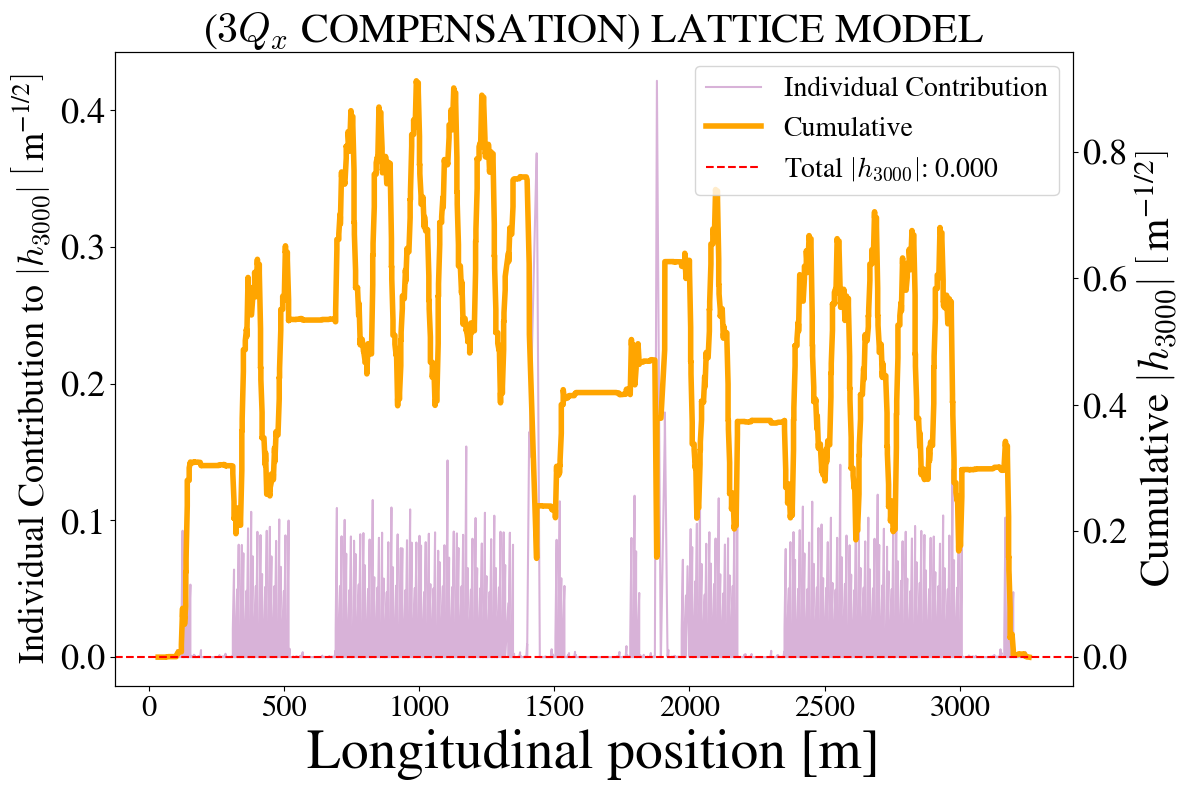
\includegraphics[width=\columnwidth]{chapter4/h3000_3qxcomp.png}
    \caption{Distribution of the $h_{3000}$ term around the ring with individual contributions from each relevant element and the cumulative sum from an arbitrary starting point when correction elements are set to compensate $3Q_x=76$, i.e., $h_{3000}=0$.}
    \label{fig:h3000_3qxcomp}
\end{figure}

On the other hand, there is the $h_{1020}$ term. This one also gets affected if normal sextupole component are changed in the lattice, as explained by the expressions in Table \ref{tab:rdts}. Therefore, it is of interest to look at how $h_{1020}$ changes as $h_{3000}$ is compensated. Figure \ref{fig:h1020_3qxcomp} shows the calculation for this term as $3Q_x$ is being compensated. Again, four additional spikes show up in the individual contribution plot exactly where the compensation sextupoles are placed. If this plot is compared to Fig. \ref{fig:h1020bare}, it can also be seen that the total sum of the $h_{1020}$ term increases from 1.739 to 1.988 m$^{-1/2}$. This shows that by compensating the $h_{3000}$ RDT, the $h_{1020}$ increases. This means that by compensating one resonance line, other lines might get worse. 

\begin{figure}[H]
    \centering
    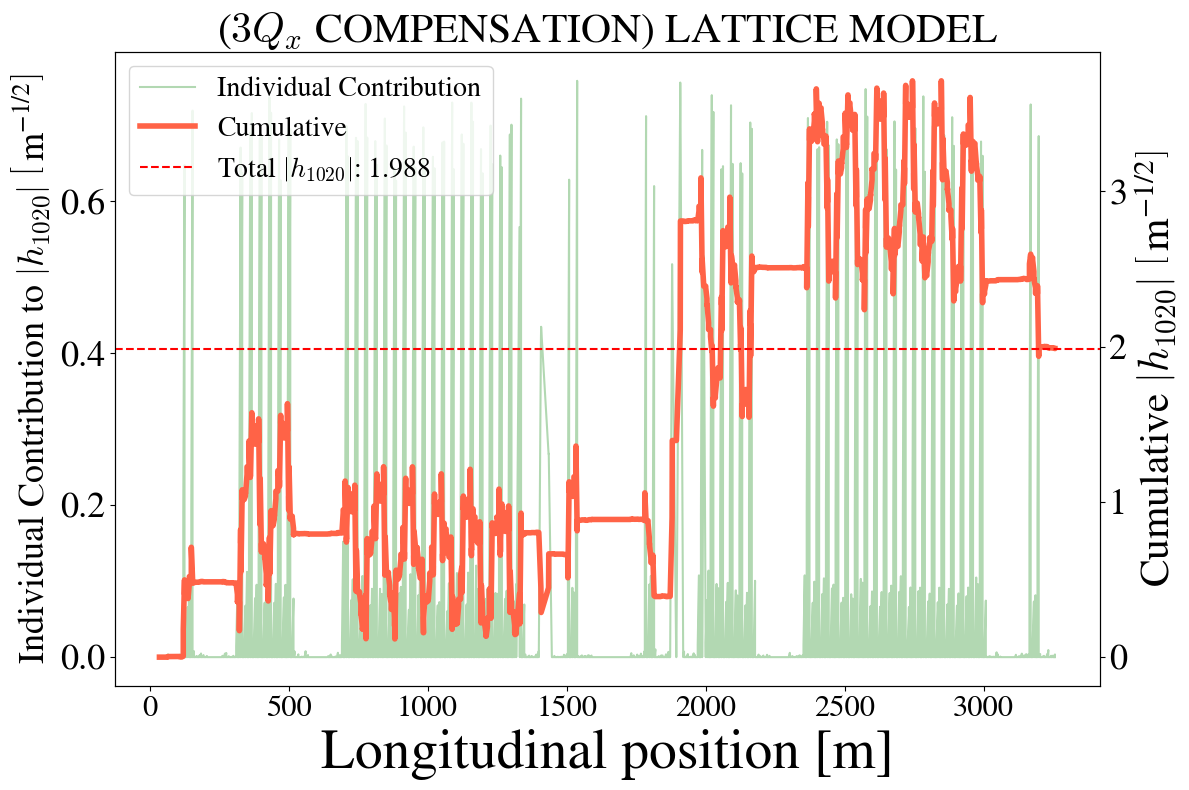
\includegraphics[width=\columnwidth]{chapter4/h1020_3qxcomp.png}
    \caption{Distribution of the $h_{1020}$ term around the ring with individual contributions from each relevant element and the cumulative sum from an arbitrary starting point when correction elements are set to compensate $3Q_x=76$, i.e., $h_{3000}=0$.}
    \label{fig:h1020_3qxcomp}
\end{figure}

An effort can be done to extend Eq. \ref{eq:model1} to include the cancellation of $h_{1020}$. The simultaneous compensation of the $h_{3000}$ and the $h_{1020}$ term is given by the following equation:
\begin{equation}
    \begin{bmatrix}
        -|h_{3000}| \cos \psi_{3000} \\
        -|h_{3000}| \sin \psi_{3000} \\
        -|h_{1020}| \cos \psi_{1020} \\
        -|h_{1020}| \sin \psi_{1020} \\
        \end{bmatrix}_{(Bare)}
         =
        \boldsymbol{M}
        \begin{bmatrix}
        K_2^{(sc220)} \\
        K_2^{(sc222)}\\
        K_2^{(sc319)} \\
        K_2^{(sc321)}\\
        \end{bmatrix}.
        \label{eq:model2}
\end{equation}
For this case, the response matrix $\boldsymbol{M}$ needs to be modified. This new response matrix reads:
\begin{equation}
    \boldsymbol{M} = 
\begin{bmatrix}

M_{11} && M_{12} && M_{13} && M_{14}  \\ 

M_{21} && M_{22} && M_{23} && M_{24} \\ 

M_{31} && M_{32} && M_{33} && M_{34}  \\ 

M_{41} && M_{42} && M_{43} && M_{44} \\ 

\end{bmatrix},
\label{eq:rm2}
\end{equation}
where the first two rows are defined the same as before by Eqs. \ref{eq:M12}-\ref{eq:M24}. Similarly, the coefficients in the last two rows are defined by:
\begin{equation}
    M_{31}=\frac{1}{16} l_{sc} \: \beta^{1/2}_{x(sc220)} \beta_{y(sc220)} \: \cos \left( \phi_{x(sc220)} + 2\phi_{y(sc220)} \right),
    \label{eq:M31}
\end{equation}
\begin{equation}
    M_{32}=\frac{1}{16} l_{sc} \: \beta^{1/2}_{x(sc222)} \beta_{y(sc222)} \: \cos \left( \phi_{x(sc222)} + 2\phi_{y(sc222)} \right),
    \label{eq:M32}
\end{equation}
\begin{equation}
    M_{33}=\frac{1}{16} l_{sc} \: \beta^{1/2}_{x(sc319)} \beta_{y(sc319)} \: \cos \left( \phi_{x(sc319)} + 2\phi_{y(sc319)} \right),
    \label{eq:M33}
\end{equation}
\begin{equation}
    M_{34}=\frac{1}{16} l_{sc} \: \beta^{1/2}_{x(sc321)} \beta_{y(sc321)} \: \cos \left( \phi_{x(sc321)} + 2\phi_{y(sc321)} \right),
    \label{eq:M34}
\end{equation}
\begin{equation}
    M_{41}=\frac{1}{16} l_{sc} \: \beta^{1/2}_{x(sc220)} \beta_{y(sc220)} \: \sin \left( \phi_{x(sc220)} + 2\phi_{y(sc220)} \right),
    \label{eq:M41}
\end{equation}
\begin{equation}
    M_{42}=\frac{1}{16} l_{sc} \: \beta^{1/2}_{x(sc222)} \beta_{y(sc222)} \: \sin \left( \phi_{x(sc222)} + 2\phi_{y(sc222)} \right),
    \label{eq:M42}
\end{equation}
\begin{equation}
    M_{43}=\frac{1}{16} l_{sc} \: \beta^{1/2}_{x(sc319)} \beta_{y(sc319)} \: \sin \left( \phi_{x(sc319)} + 2\phi_{y(sc319)} \right),
    \label{eq:M43}
\end{equation}
\begin{equation}
    M_{44}=\frac{1}{16} l_{sc} \: \beta^{1/2}_{x(sc321)} \beta_{y(sc321)} \: \sin \left( \phi_{x(sc321)} + 2\phi_{y(sc321)} \right),
    \label{eq:M44}
\end{equation}
as calculated from the derivative of $h_{1020}$ with respect to $K_2^{(i)}$, with the explicit expression in Table \ref{tab:rdts}.

The solution to Eq. \ref{eq:model2} is just given by the inverse of the response matrix applied to the bare machine RDT vector. This is equivalent to the approach in Eq. \ref{eq:model1sol}. The result of this approach is the calculation of the $K_2$ coefficients in the compensation sextupoles that cancel out, both, the $h_{3000}$ and the $h_{1020}$ term. The solution to Eq. \ref{eq:model2} is given in Table \ref{tab:k2sboth} for an arbitrarily tuned lattice. One thing to note is that these values are almost one order of magnitude larger than those in Table \ref{tab:k2sh3000}. 

\begin{table}[H]
    \centering
    \caption{$K_2$ coefficients that cancel out the $h_{3000}$ and $h_{1020}$ term. These values were calculated for a Recycler lattice tuned to $Q_x=25.4422$ and $Q_y=24.3915$.}
    \label{tab:k2sboth}
    \begin{tabular}{cc}
    \toprule
    \textbf{Sextupole} & $K_2$ [m$^{-3}$] \\ \midrule
     &  \\
    SC220 & 6.039888 \\
     &  \\
    SC222 & 4.826964 \\
     &  \\
    SC319 & -4.529674 \\
     &  \\
    SC321 & -6.167827 \\
     &  \\ \hline
    \end{tabular}
    \end{table}

Once the magnet coefficients from Table \ref{tab:k2sboth} are input into the lattice model, the RDT calculations can be done to verify that the terms effectively go to 0. Figures \ref{fig:h3000oldconfig} and \ref{fig:h1020oldconfig} show these calculations. And, indeed, one can see how the RDT sums add up to 0. Nevertheless, it can be seen from these plots how the spikes are now very large compared to the previous cases and compared to the individual contributions from around the lattice. Effectively, this means that the sextupole component will be localized in the compensation sextupoles' locations. This is an unwanted effect, given that these large sextupole kicks will result in overfocusing of the beam in these locations. In particular, the sextupole component will no longer be perturbative in these locations. 

\begin{figure}[H]
    \centering
    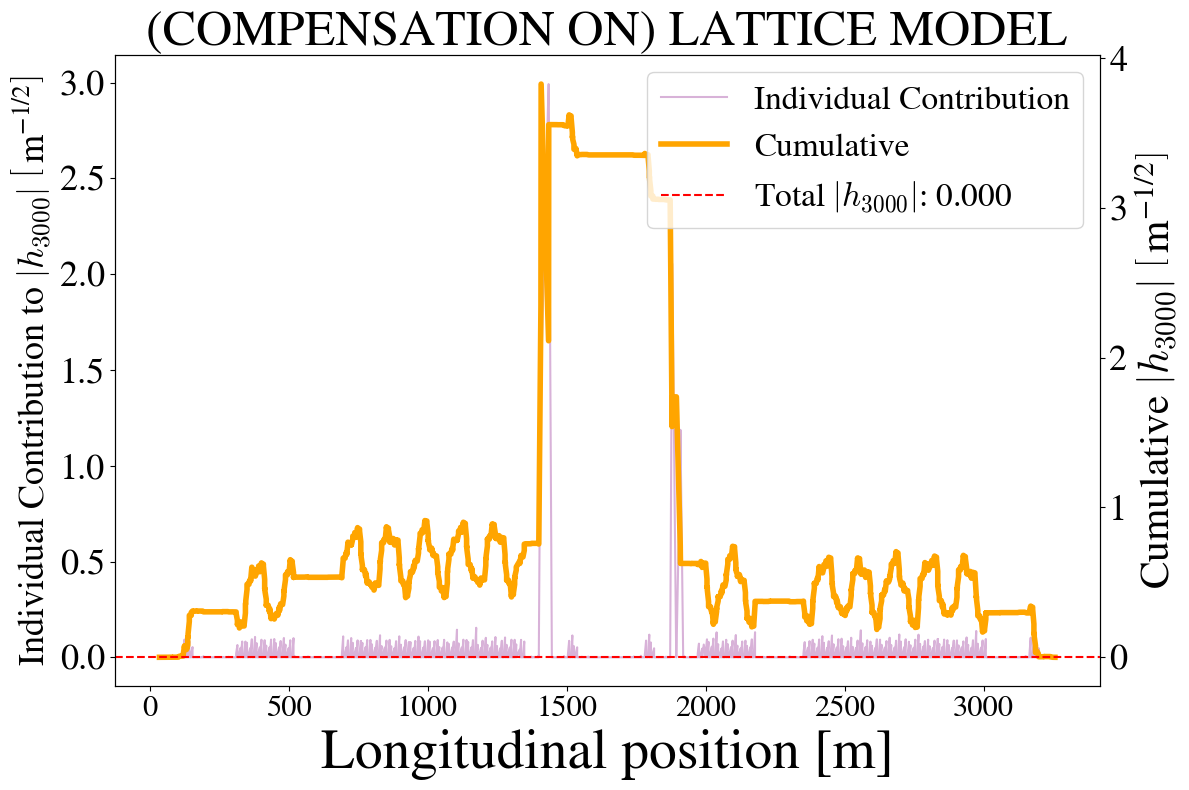
\includegraphics[width=\columnwidth]{chapter4/old_config_h3000.png}
    \caption{Distribution of the $h_{3000}$ term around the ring with individual contributions from each relevant element and the cumulative sum from an arbitrary starting point. This is with existing sextupoles powered at the correct currents to cancel out $h_{3000}$ and $h_{1020}$ simultaneously.}
    \label{fig:h3000oldconfig}
\end{figure}

The results from solving Eq. \ref{eq:model2}, as specified in Table \ref{tab:k2sboth}, indicate that the $K_2$ coefficients are very large compared to the case where there was only $h_{3000}$ compensation. Experimentally, what is observed is that the currents in the sextupoles that compensate both $h_{3000}$ and $h_{1020}$ are too large, and they exceed the range of operational limits. While there are no limits for $K_2$ in the sextupoles from the lattice model, the solutions are very large. If one were to translate the operational current limits of the sextupoles to the lattice model $K_2$ coefficients, it can be shown that the solutions lie out of this range, i.e., the maximum $K_2$ coefficients are around 1 m$^{-3}$. Therefore, this solution does not work for the operational beam. Section \ref{sec:addsexts} shows how to circumvent this by adding two additional sextupoles in the lattice at optimized locations in order to bring down the compensation $K_2$ coefficients---effectively, the compensation currents.

\begin{figure}[H]
    \centering
    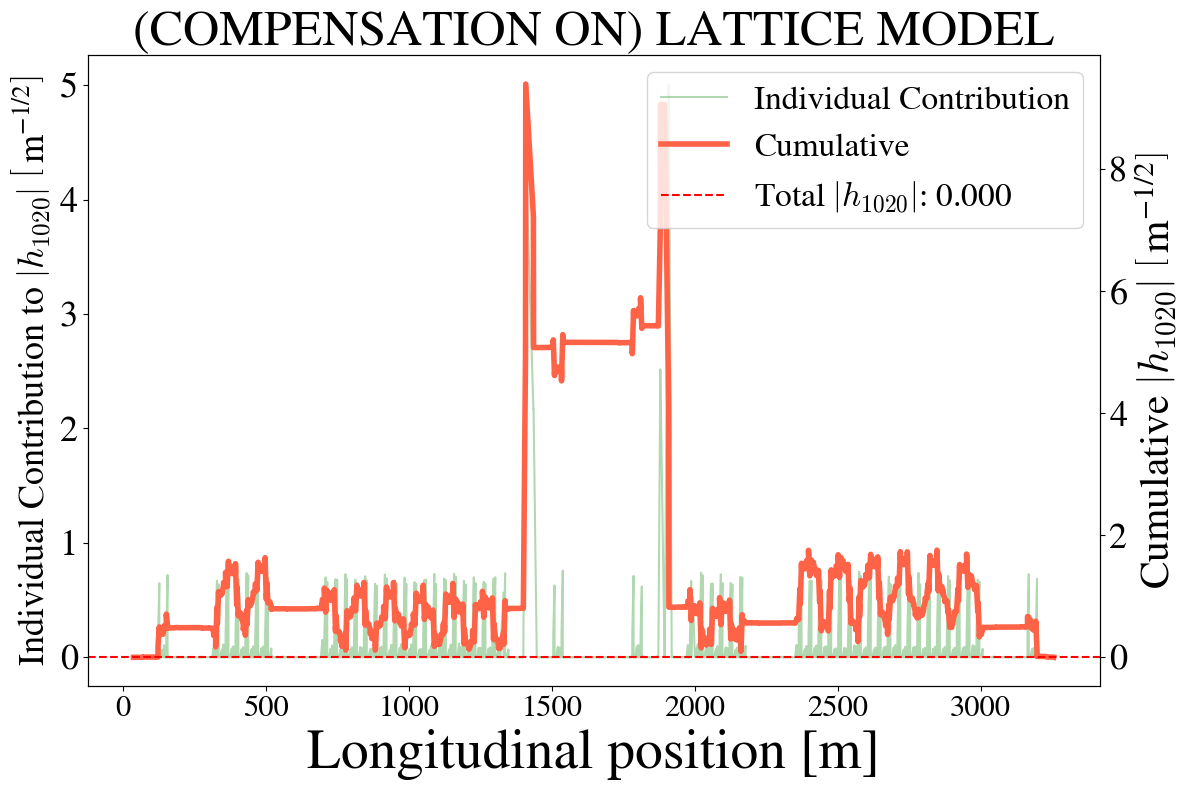
\includegraphics[width=\columnwidth]{chapter4/old_config_h1020.png}
    \caption{Distribution of the $h_{1020}$ term around the ring with individual contributions from each relevant element and the cumulative sum from an arbitrary starting point. This is with existing sextupoles powered at the correct currents to cancel out $h_{3000}$ and $h_{1020}$ simultaneously.}
    \label{fig:h1020oldconfig}
\end{figure}

While the previous section, focused only on the normal sextupole RDTs, all of this can easily be extended to the skew sextupole RDTs, i.e., $h_{0030}$ and $h_{2010}$. This is assuming the lattice model has a good approximation of the skew sextupole distribution around the ring. For the Recycler Ring, the skew sextupole resonances are not as strong as the normal sextupole resonance $3Q_x=76$. This resonance dominates the losses in this region. Therefore, special attention has been paid to the $3Q_x=76$ resonance and its $h_{3000}$ resonance driving term. Nevertheless, this procedure works for $3Q_y=73$ and $2Q_x+Q_y=75$---and its corresponding RDTs---using the skew sextupole correctors.

\subsection{Response Matrix Approach}

The next step is to look at how to translate the procedure from the previous section to the real machine. This is done by means of measuring the response matrix. As mentioned before, for resonance compensation there are four dedicated normal sextupoles with currents that can be set to ($I_{sc220},I_{sc222},I_{sc319},I_{sc321}$) and four dedicated skew sextupoles with currents that can be set to ($I_{ss323},I_{ss323},I_{ss319},I_{ss321}$). As shown in the previous section one RDT can be cancelled out with the right kick from the correction elements, which means the resonances are corrected to first order. 

Nevertheless, by compensating one resonance line, other resonances might become worse. This is why for simultaneous compensation, compensation currents will vary depending on the subsets of resonances to compensate. In principle, the currents $I_x$ needed in each correction element in order to cancel out the four bare machine RDTs, are given by the solution to this linear system of equations: 
\begin{equation}
    \begin{bmatrix}
        -|{h_{3000}}|  \cos (\psi_{3000})\\
        -|{h_{3000}}|  \sin (\psi_{3000})\\
        -|{h_{1020}}|  \cos (\psi_{1020})\\
        -|{h_{1020}}|  \sin (\psi_{1020})\\
        -|{h_{0030}}|  \cos (\psi_{3000})\\
        -|{h_{0030}}|  \sin (\psi_{3000})\\
        -|{h_{2010}}|  \cos (\psi_{1020})\\
        -|{h_{2010}}|  \sin (\psi_{1020})\\
      \end{bmatrix}_{(Bare)}
    =
      \boldsymbol{M}
    \begin{bmatrix}
        I_{sc220} \\
        I_{sc222} \\
        I_{sc319} \\
        I_{sc321} \\
        I_{ss223} \\
        I_{ss323} \\
        I_{ss319} \\
        I_{ss321} \\
      \end{bmatrix}
    \label{eq:system}
\end{equation}
where $M_{ij}$ is the response matrix for the RDTs with respect to the currents, and includes any roll that can happen for the correction sextupoles. It is worth to emphasize that for this approach, the response matrix is being calculated from measurements as opposed to calculated from the model. This response matrix $M_{ij}$ can be calculated by scanning the currents in each correction element and looking at the response from the real and imaginary part of the RDTs, i.e., $h_{jklm}=|h_{jklm}|e^{i\psi_{jklm}}$. 

In reality, there are limitations to solving equation \ref{eq:system}. The first one is that all the RDTs ($h_{jklm}$) may not be accessible for measurement, given that they may not show up as a spectral line.  Another limitation is that the solution for the currents may be outside the maximum limits for the correction elements. 

One can also try to cancel out a subset of RDTs from equation \ref{eq:system}, including only one RDT. For example, in order to compensate $3 Q_x=76$, the system of equations to be solved is:

\begin{equation}
    \begin{bmatrix}
        -|{h_{3000}}|  \cos (\psi_{3000})\\
        -|{h_{3000}}|  \sin (\psi_{3000})\\
        0\\
        0\\
      \end{bmatrix}_{(Bare)}
    =
    \begin{bmatrix}
        M_{11} & M_{12} & M_{13} & M_{14} \\
        M_{21} & M_{22} & M_{23} & M_{24} \\
        1 & 1 & 0 & 0 \\
        0 & 0 & 1 & 1 \\
    \end{bmatrix}
    \begin{bmatrix}
        I_{sc220} \\
        I_{sc222} \\
        I_{sc319} \\
        I_{sc321} \\
      \end{bmatrix},
    \label{eq:system1}
\end{equation}
which is analogous to Eq. \ref{eq:model1}, only now the sextupole currents are the knobs. Nevertheless, in this case, the RDT is measured from the procedure shown in Sec. \ref{sec:rdtmeasure} for the bare machine---no compensation sextupoles turned on. In order to measure the response matrix $\boldsymbol{M}$, the $h_{3000}$ RDT has to be measured as a function of the compensation currents in the sextupoles. The procedure summarizing all of this is the following:
\begin{enumerate}
    \item Measure the bare machine RDT vector for several shots, e.g, measure $h_{3000}$ for 20 instances.
    \item Choose a compensation sextupole for the first scan.
    \item Set the compensation sextupole to the lower limit of the scan range, e.g., -10 Amps.
    \item Measure the $h_{3000}$ RDT (or arbitrary RDT) by means of following the recipe in Sec. \ref{sec:rdtmeasure}.
    \item Increase the current in the compensation sextupole by some step size, e.g., by 2 Amps, and repeat the RDT measurement.
    \item Repeat steps 2-4 until the upper limit of the scan range, e.g., 10 Amps.
    \item For every measurement, decompose the RDT into its real and imaginary part, e.g., $h_{3000}= |h_{3000}| \cos \psi_{3000} + i |h_{3000}| \sin \psi_{3000}$. 
    \item Plot the real and imaginary part of the RDT as a function of sextupole current and perform a linear fit. The slopes of these fits are the corresponding $M_{ij}$ response matrix coefficients.
    \item Repeat steps 2-8 for the other compensation sextupoles, until the response matrix is fully calculated. This procedure can be done for a subset of correctors reducing the dimension of the response matrix. 
    \item Once the response matrix is specified, calculate its inverse (or pseudo-inverse) and operate on to the bare machine RDT vector in order to get the compensation currents on every BPM (see Fig. \ref{fig:icomp}).
\end{enumerate}

Figures \ref{fig:h3000_sc222} and \ref{fig:h3000_sc319} shows an example of performing two of these scans for the $h_{3000}$ term. On Fig. \ref{fig:h3000_sc222} it can be seen how the relationship between the real part and imaginary part follow a linear relation within the shaded region. The fit for these plots was done only for this region given that prior empirical data showed that the currents should not exceed the absolute value of 7 Amps. The response matrix coefficients were extracted for the slope values provided from the fit.  

\begin{figure}[H]
    \centering
    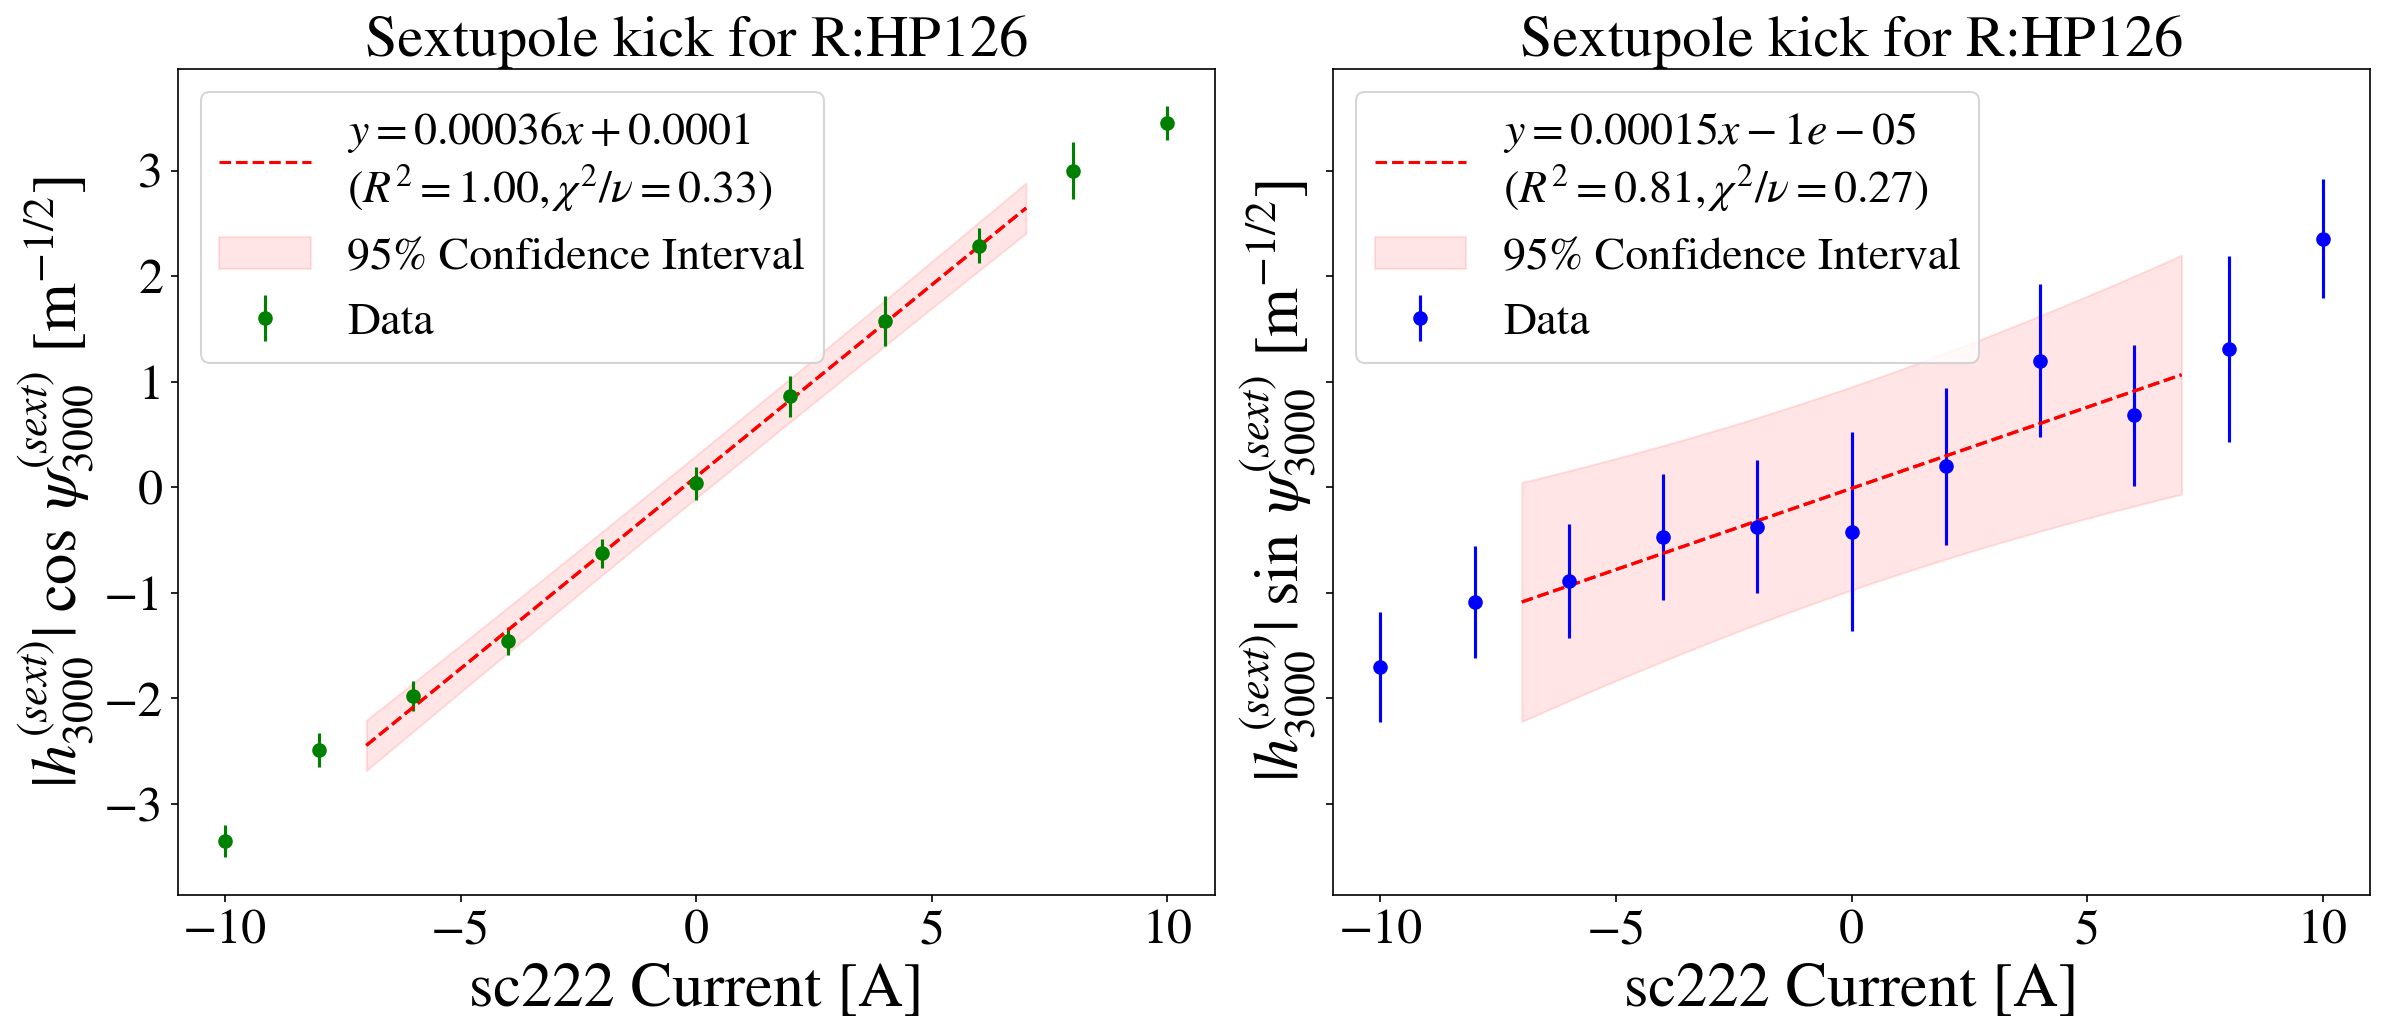
\includegraphics[width=\columnwidth]{chapter4/h3000_sc222.png}
    \caption{Real and imaginary part of $h_{3000}$ as a function of current fed to compensation sextupole SC222. Measurement is shown for R:HP126 data.}
    \label{fig:h3000_sc222}
\end{figure}

Figures \ref{fig:h3000_sc222} and \ref{fig:h3000_sc319} are taken at two different BPMs, i.e., horizontal BPMs R:HP126 and R:HP612. Comparing both plots, shows that the RDT sensitivity of $h_{3000}$ changes depending on the sextupole used. Furthermore, at high currents it can be seen that some non-linear behavior starts to kick in. This was present in mostly all BPMs. Nevertheless, this only happened at high currents far from the region of interest, which was capped at an absolute value of 6 Amps. 

After performing all this process, the result is an array of compensating currents predicted by every BPM. Figure \ref{fig:icomp} shows an example of these results. The bars at each BPM represent the predicted compensation current for a particular sextupole. While each BPM will give a local approximation of what currents minimize the $h_{3000}$ RDT, the sextupoles can only take one input. This is why all these currents need to be averaged in order to get a global compensation current that minimizes the RDT at every location. Nevertheless, given that there is some uncertainty on the bare machine RDTs and the response matrix coefficients, this needs to be included in order to come up with this global solution. 

\begin{figure}[H]
    \centering
    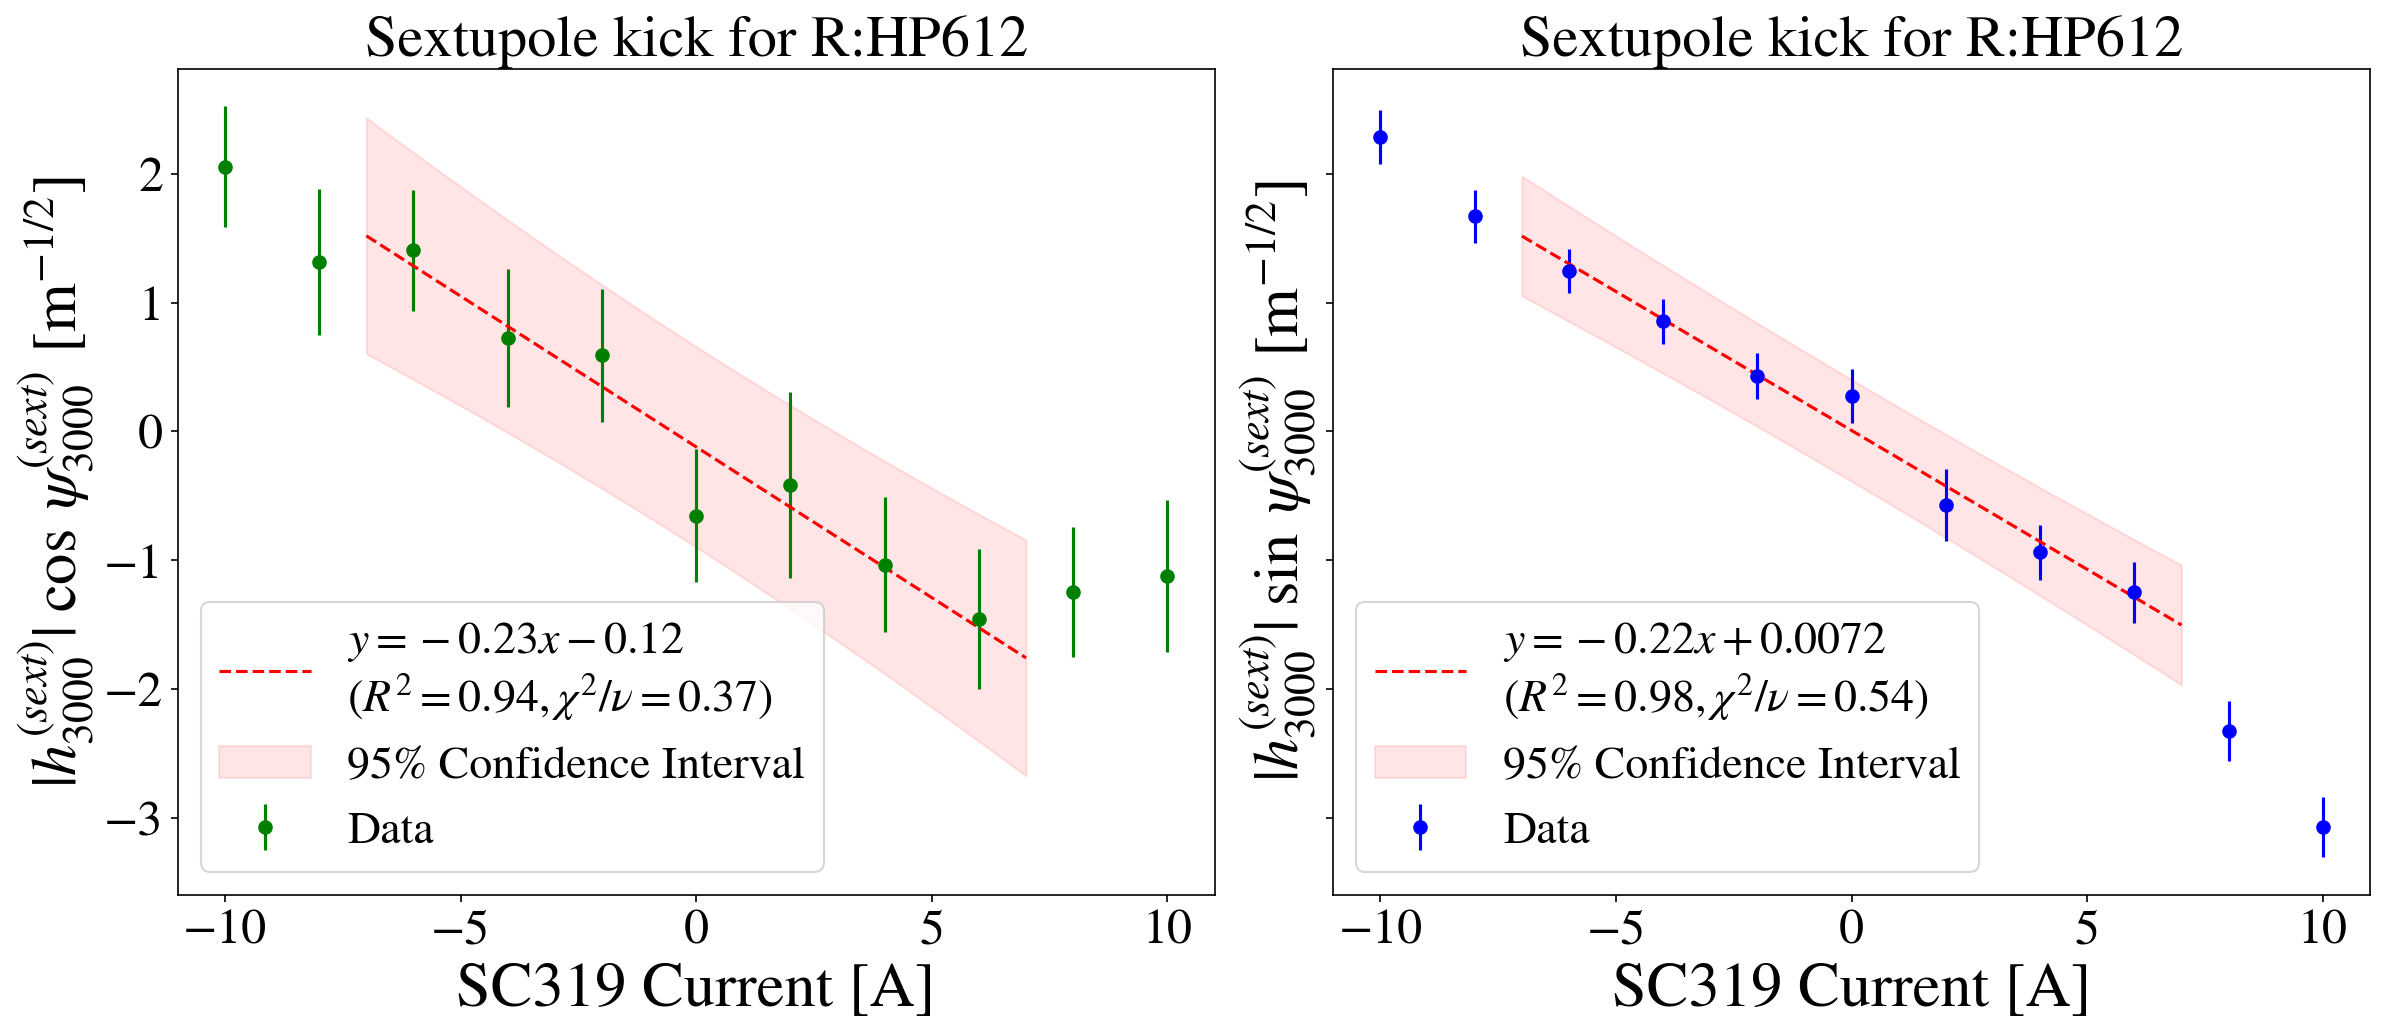
\includegraphics[width=\columnwidth]{chapter4/h3000_sc319.png}
    \caption{Real and imaginary part of $h_{3000}$ as a function of current fed to compensation sextupole SC319. Measurement is shown for R:HP612 data.}
    \label{fig:h3000_sc319}
\end{figure}

In order to build a final setting for the compensation currents, not all BPMs are necessarily used. For this prediction, the BPMs that showed the most linear fits from the RDT scan as a function of current were used. The R-squared statistics and the reduced $\chi^2$ were used to quantify this linearity. Once the best BPMs were selected, the compensation currents were selected. This is why not all BPMs are plotted on Fig. \ref{fig:icomp}. Assuming that the currents predictions shown in Fig. \ref{fig:icomp} follow a bi-Gaussian distribution centered at the mean values with a variance equal to the uncertainty in the error bar, a prediction function can be built. The prediction function is just the sum of all the bi-Gaussian distributions. A contour plot example of such prediction function is shown in Fig. \ref{fig:icomp_int}. Ultimately, this prediction function will specify a region in the currents space of each sextupole where the best setting lies.

\begin{figure}[H]
    \centering
    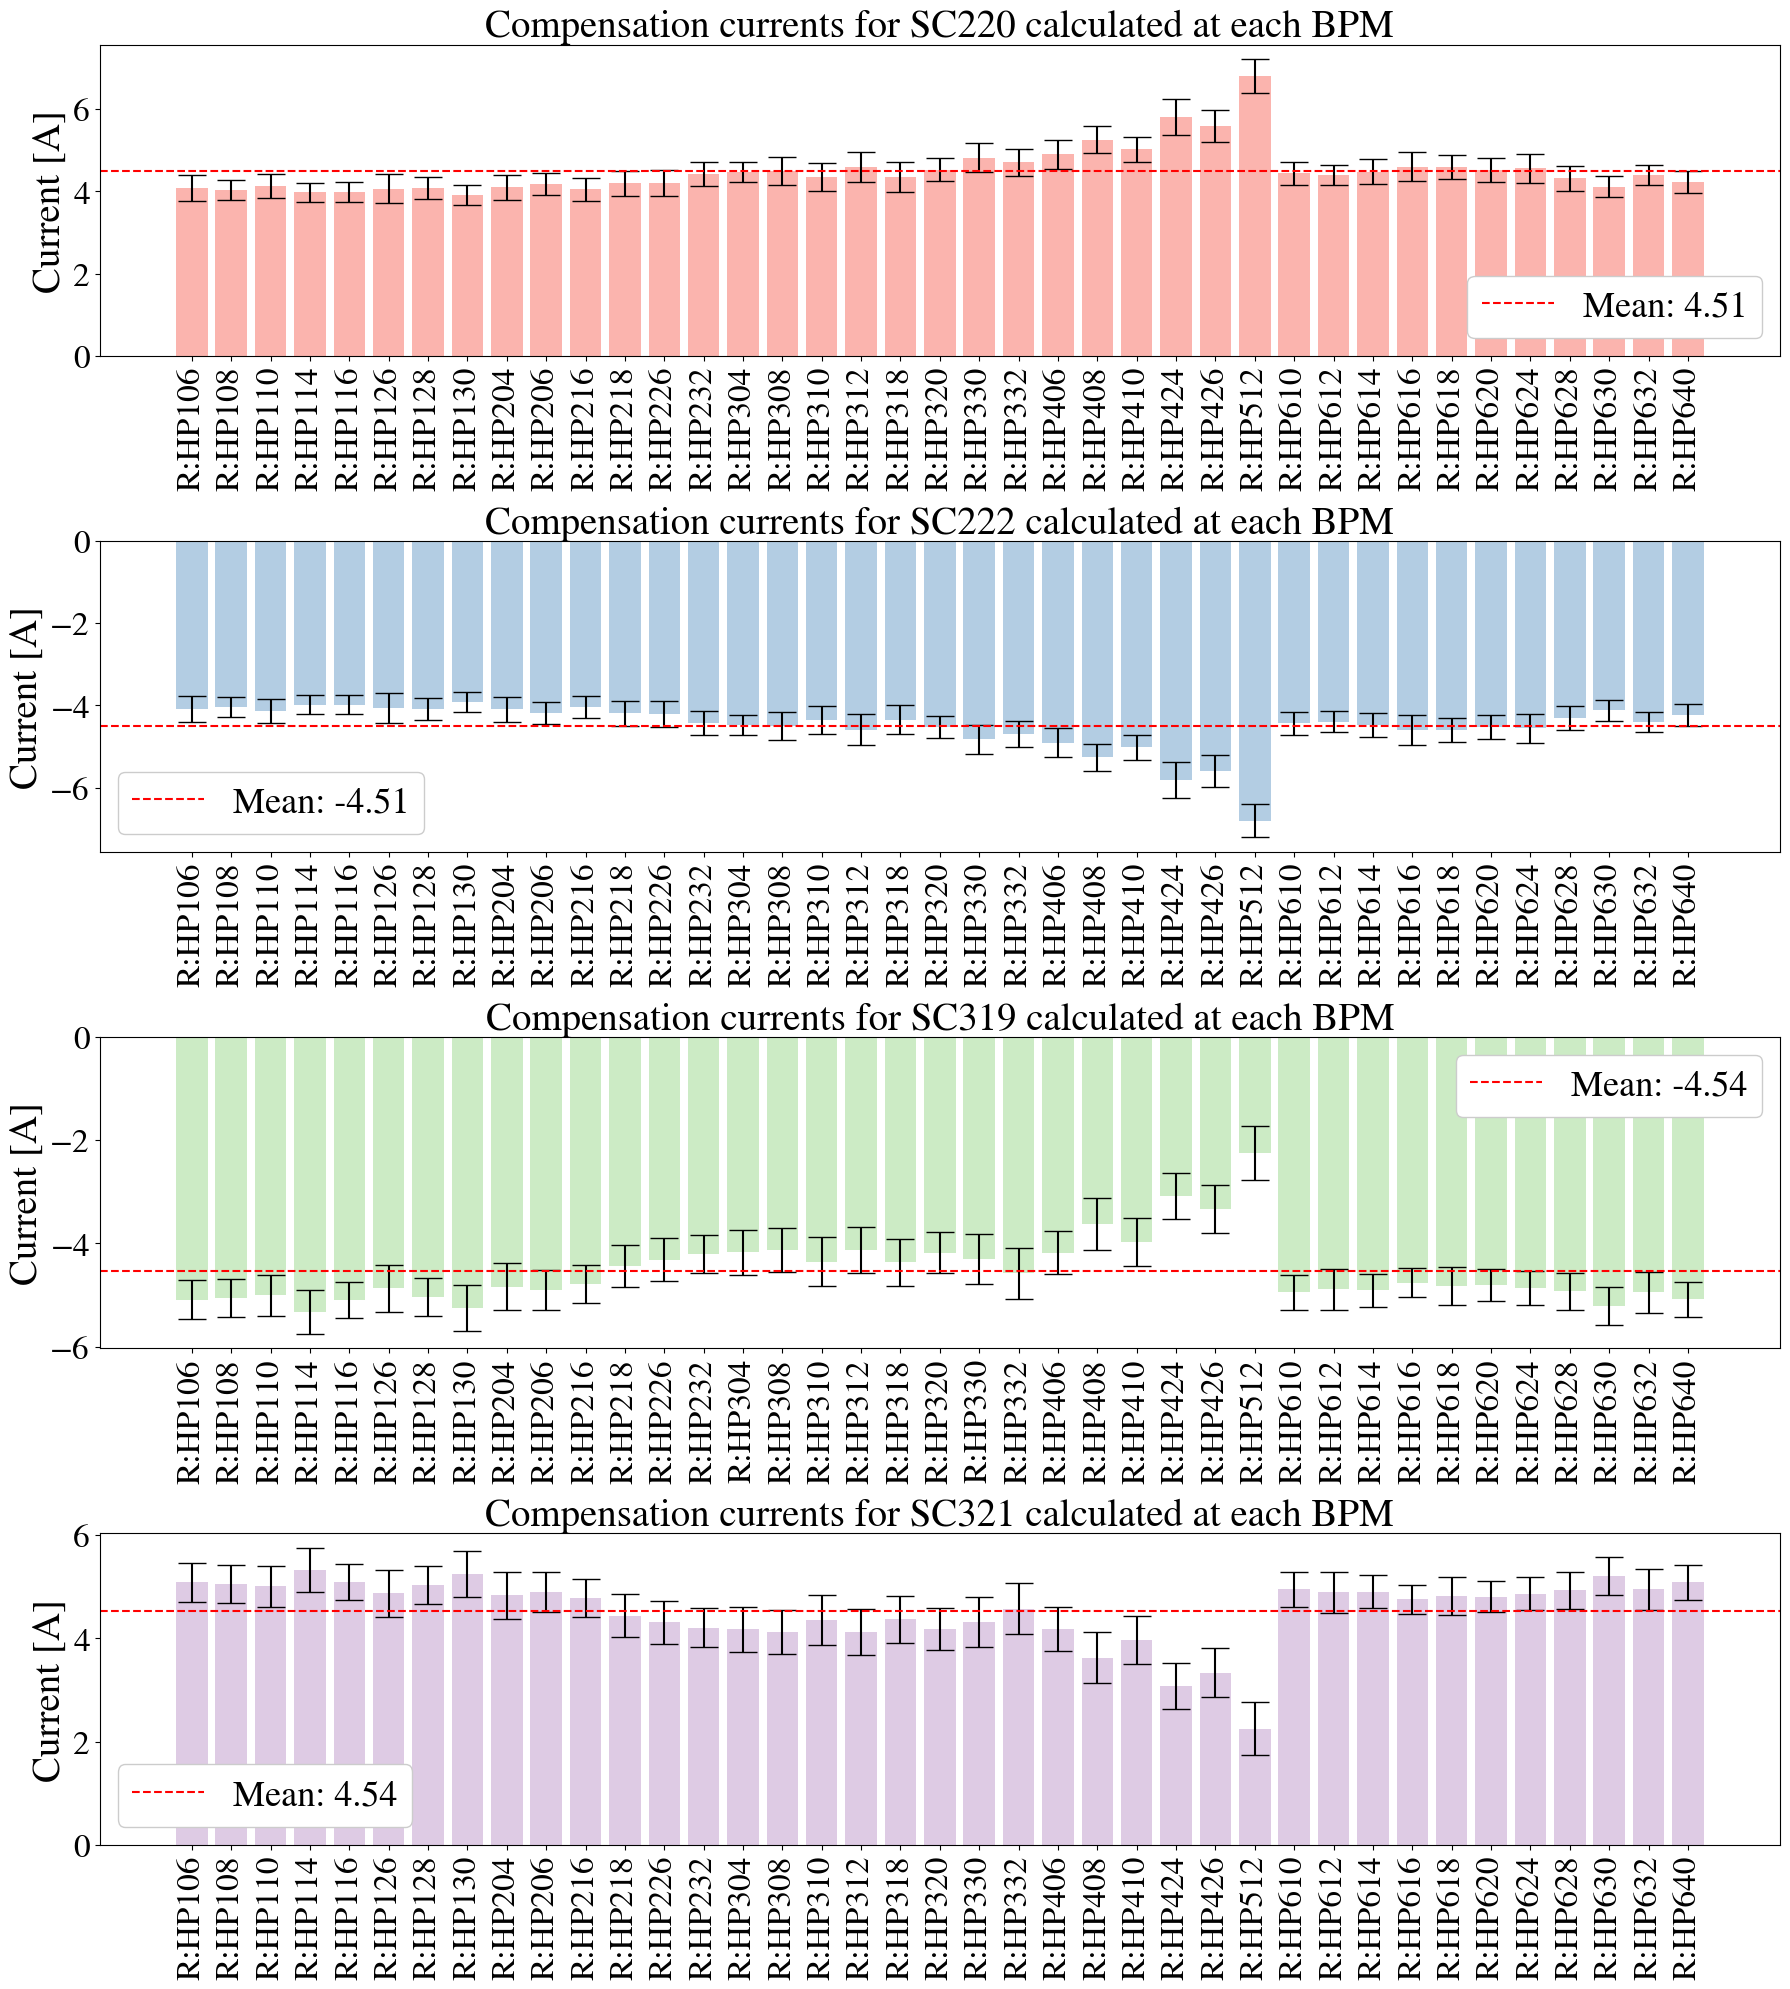
\includegraphics[width=\columnwidth]{chapter4/comp_currents.png}
    \caption{Compensation currents calculated from BPMs that showed the best R-square statistic from performing the RDT scans.}
    \label{fig:icomp}
\end{figure}

\begin{figure}[H]
    \centering
    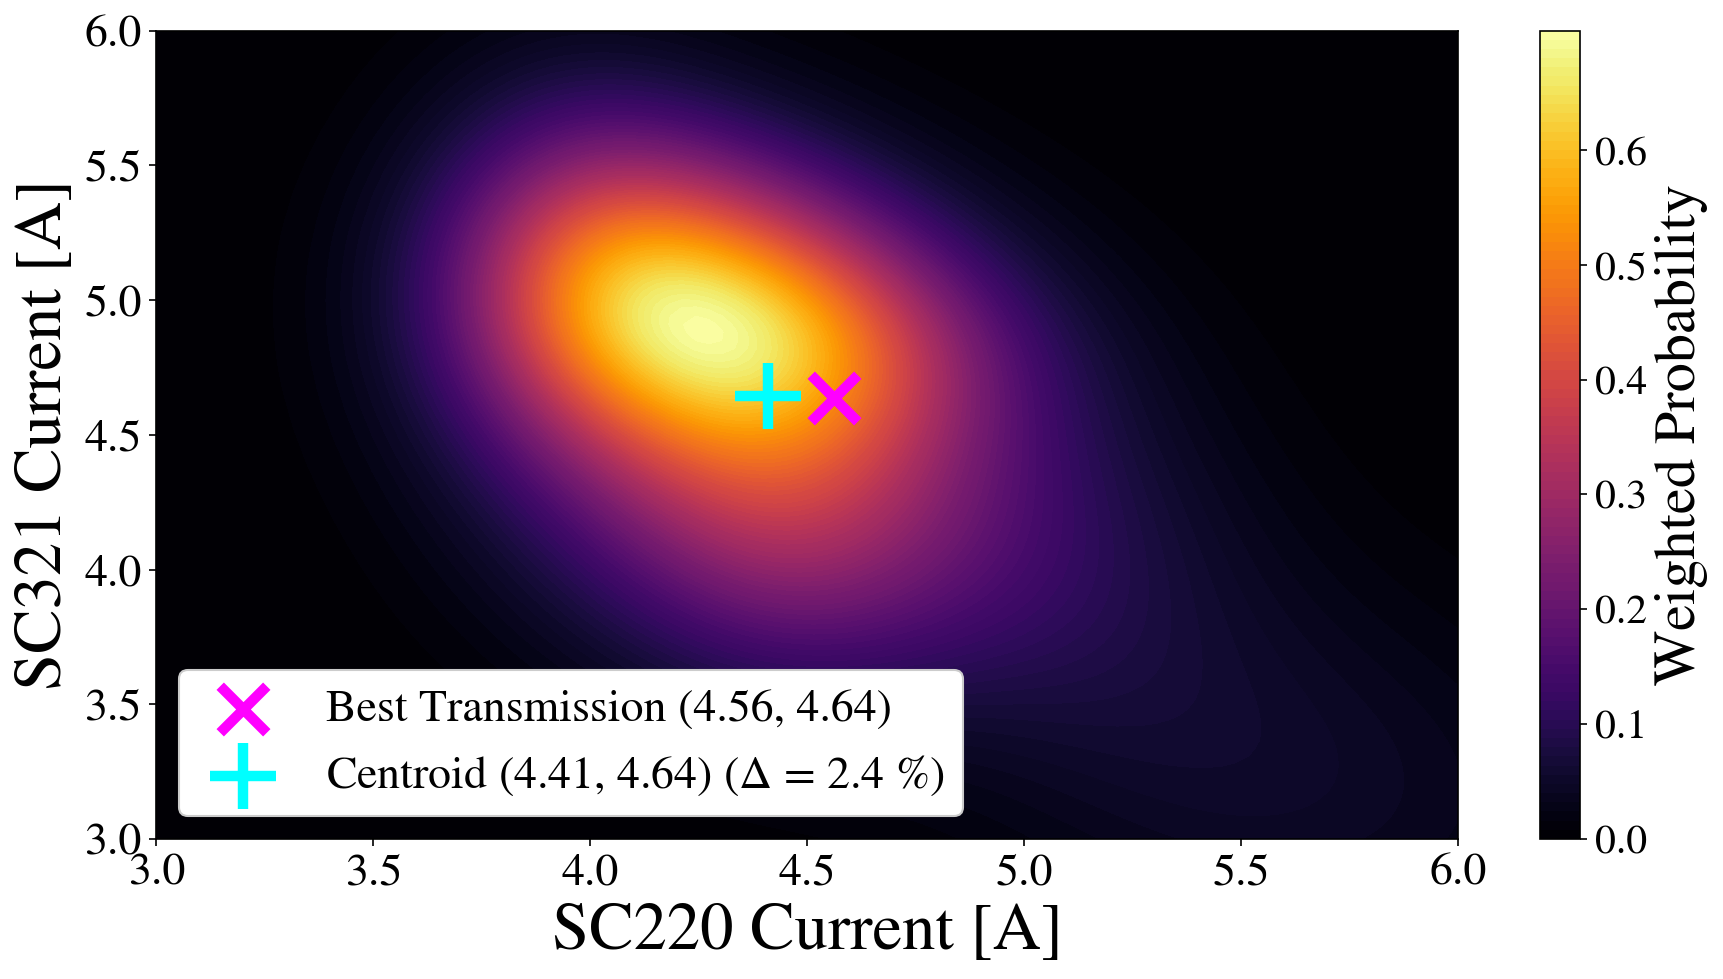
\includegraphics[width=\columnwidth]{chapter4/comp_interval.png}
    \caption{Prediction function built from the best R-squared statistics BPMs, in order to predict the best global currents for $h_{3000}$ compensation.}
    \label{fig:icomp_int}
\end{figure}

The prediction function in Fig. \ref{fig:icomp_int} can be used to predict an optimal setting for the currents in the compensation sextupoles. Specifically, the centroid of this prediction distribution can be calculated and used as the optimum setting. This corresponds to the cyan cross in Fig. \ref{fig:icomp_int}. Later in this chapter, there is a whole section dedicated to verify the compensation of resonances, see Sec. \ref{sec:verify}. Nevertheless, a quick way to verify resonance compensation is to use a dynamic tune ramp that crosses the $3Q_x=76$. Uncorrected for, around 95\% of the beam is lost once this resonance is crossed. One can use the interval where the prediction function thinks it is best to operate, and scan the parameter space (currents) while recording beam transmission across the $3Q_x$ resonance. The fuchsia X in Fig. \ref{fig:icomp_int} shows the setting with the best transmission---the best transmission now corresponds to less than 5\% losses. The centroid of the prediction function is around 2.4\% (relative distance) away from this experimental value. This shows that the predicted value from the response matrix approach does indeed reduce the losses from the $3Q_x=76$ line---meaning the $h_{3000}$ RDT is minimized in this region.

\section{Optimization of Compensation Currents}

The last section showed how to predict the optimum setting for the sextupoles by measuring the response matrix. Nevertheless, this procedure takes a couple of hours of study time and might not be accessible for routine operations. Therefore, this procedure might be done once or twice per run. Consequently, it is of interest to explore optimization algorithms that can help predict the optimum setting that minimizes losses from the resonance lines.   

\begin{figure}[H]
    \centering
    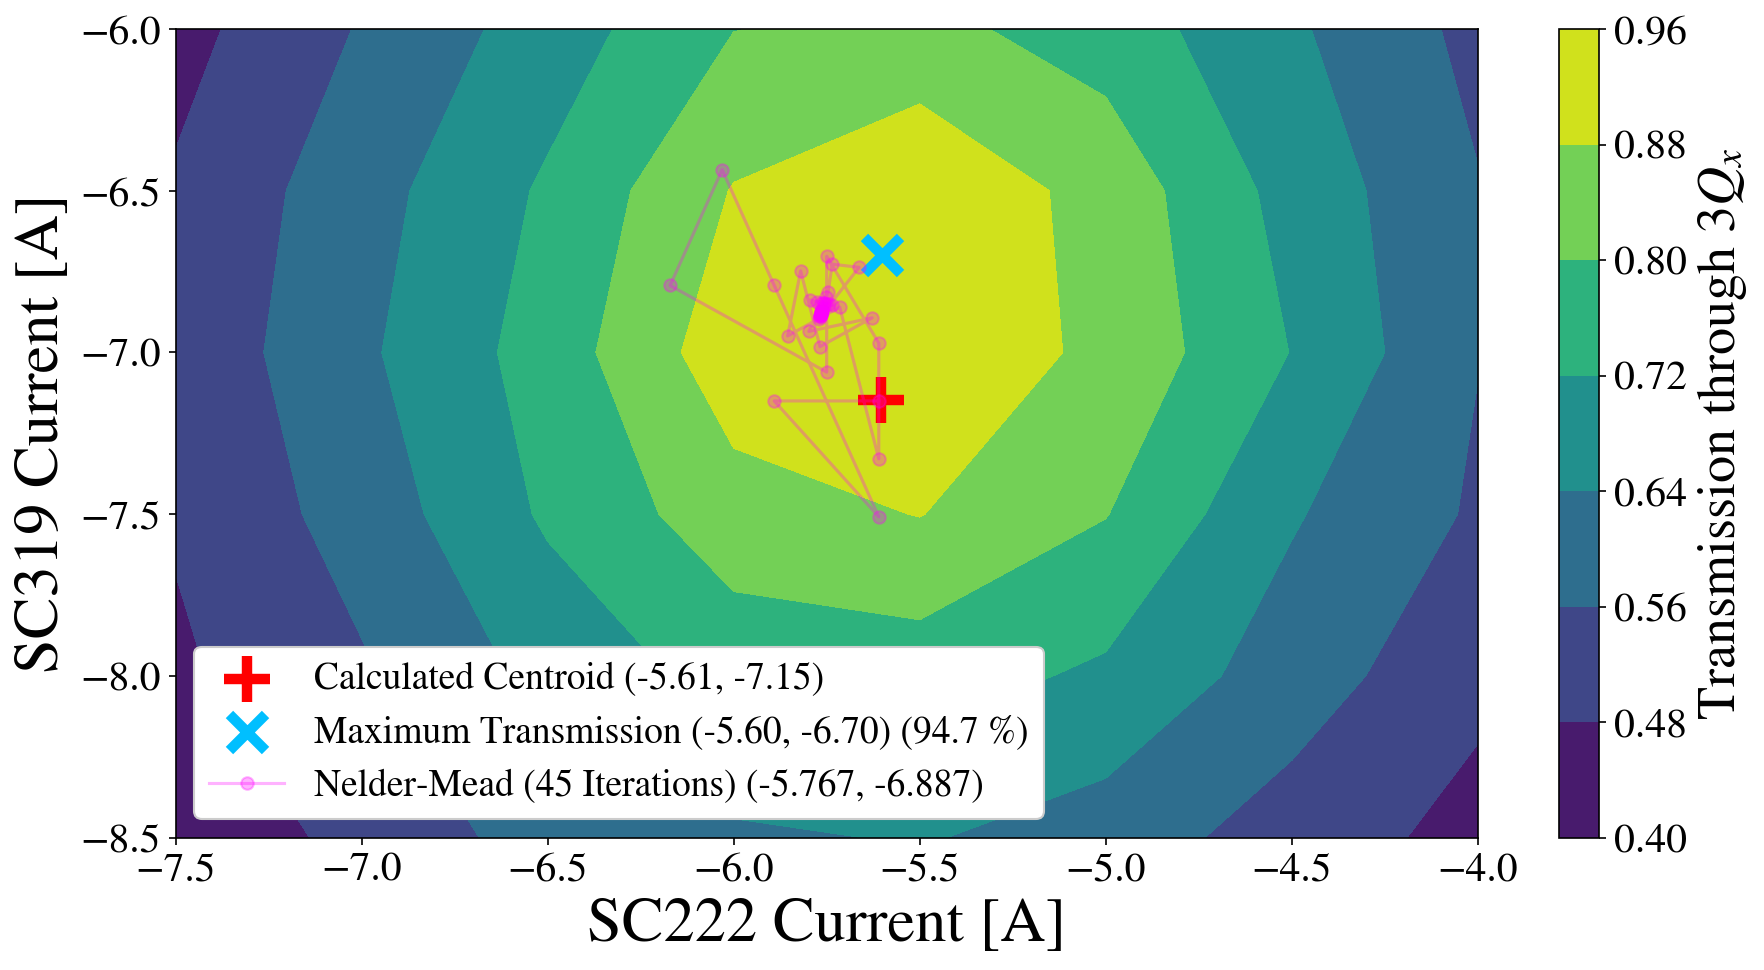
\includegraphics[width=\columnwidth]{chapter4/nelder_mead.png}
    \caption{Nelder-Mead optimization from an instance were the response matrix prediction was used as the initial point. The contour plot shows the transmission through $3Q_x$ as a function of the currents.}
    \label{fig:neldermead}
\end{figure}

Figure \ref{fig:neldermead} shows an example of using a Simplex (Nelder-Mead) optimization procedure to find the optimum setting in the compensation sextupoles. In the background of this plot, the contour plot corresponds to the experimentally-measured transmission through $3Q_x$. This Nelder-Mead instance was started with the currents predicted from the response matrix approach. After 45 iterations, the optimization algorithm converged to the value specified in the legend of Fig. \ref{fig:neldermead}. This value is fairly close to the value predicted by the response matrix approach. The maximum transmission from the contour plot (red cross in Fig. \ref{fig:neldermead}) agrees up to some significance with the currents from the optimization procedure and the response matrix approach. They're all fairly close within a region. Therefore, by taking the response-matrix predicted currents as an initial point, one can fine-tune this configuration using this type of optimization algorithms. In principle, any type of numerical optimization algorithms should converge to the answer given that the underlying function is not specially difficult---in the context of numerical optimization. 

\begin{figure}[H]
    \centering
    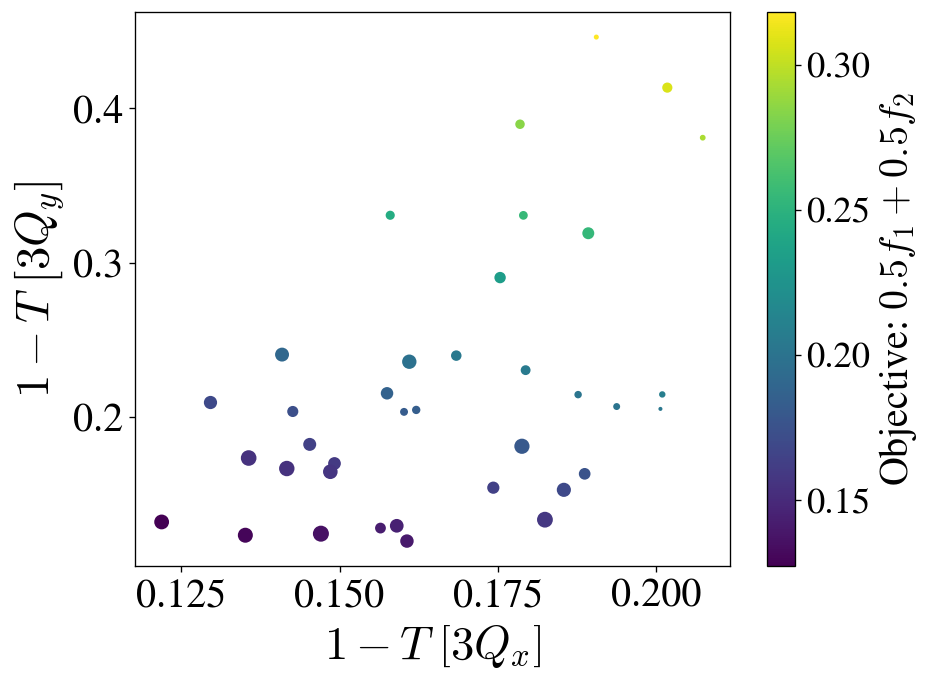
\includegraphics[width=\columnwidth]{chapter4/mo_opti.png}
    \caption{Multiobjective Nelder-Mead optimization of the transmission through $3Q_x$ and $3Q_y$. The objective function to be minimized was defined as an equally-weighted sum of both one minus transmissions---corresponding to the fractional losses through the resonance lines.}
    \label{fig:MO_neldermead}
\end{figure}

Figure \ref{fig:MO_neldermead} take this a step further by performing multiobjective optimization on two resonance lines, i.e., $3Q_x$ and $3Q_y$. The 8 compensation sextupoles (see Table \ref{tab:sextscomp}), including normal and skew, were used for this optimization. While in principle, powering up the normal compensation sextupoles should have no effect on the $3Q_y$ line, it was observed that the losses due to this line increased when $3Q_x$ was corrected. This motivated the multiobjective optimization of both lines. Figure \ref{fig:MO_neldermead} shows how by trying to correct one line the other one got worse. Ultimately, the best configuration would lie on the Pareto front of these functions. The axis in Fig. \ref{fig:MO_neldermead} represent the fractional beam loss when crossing the resonance lines. The objective function to be minimized by a Nelder-Mead algorithm was defined as an equally-weighted sum of both fractional losses. Ultimately, Fig. \ref{fig:MO_neldermead} shows how the algorithm slowly drifts toward the best solution to this problem. 

\begin{figure}[H]
    \centering
    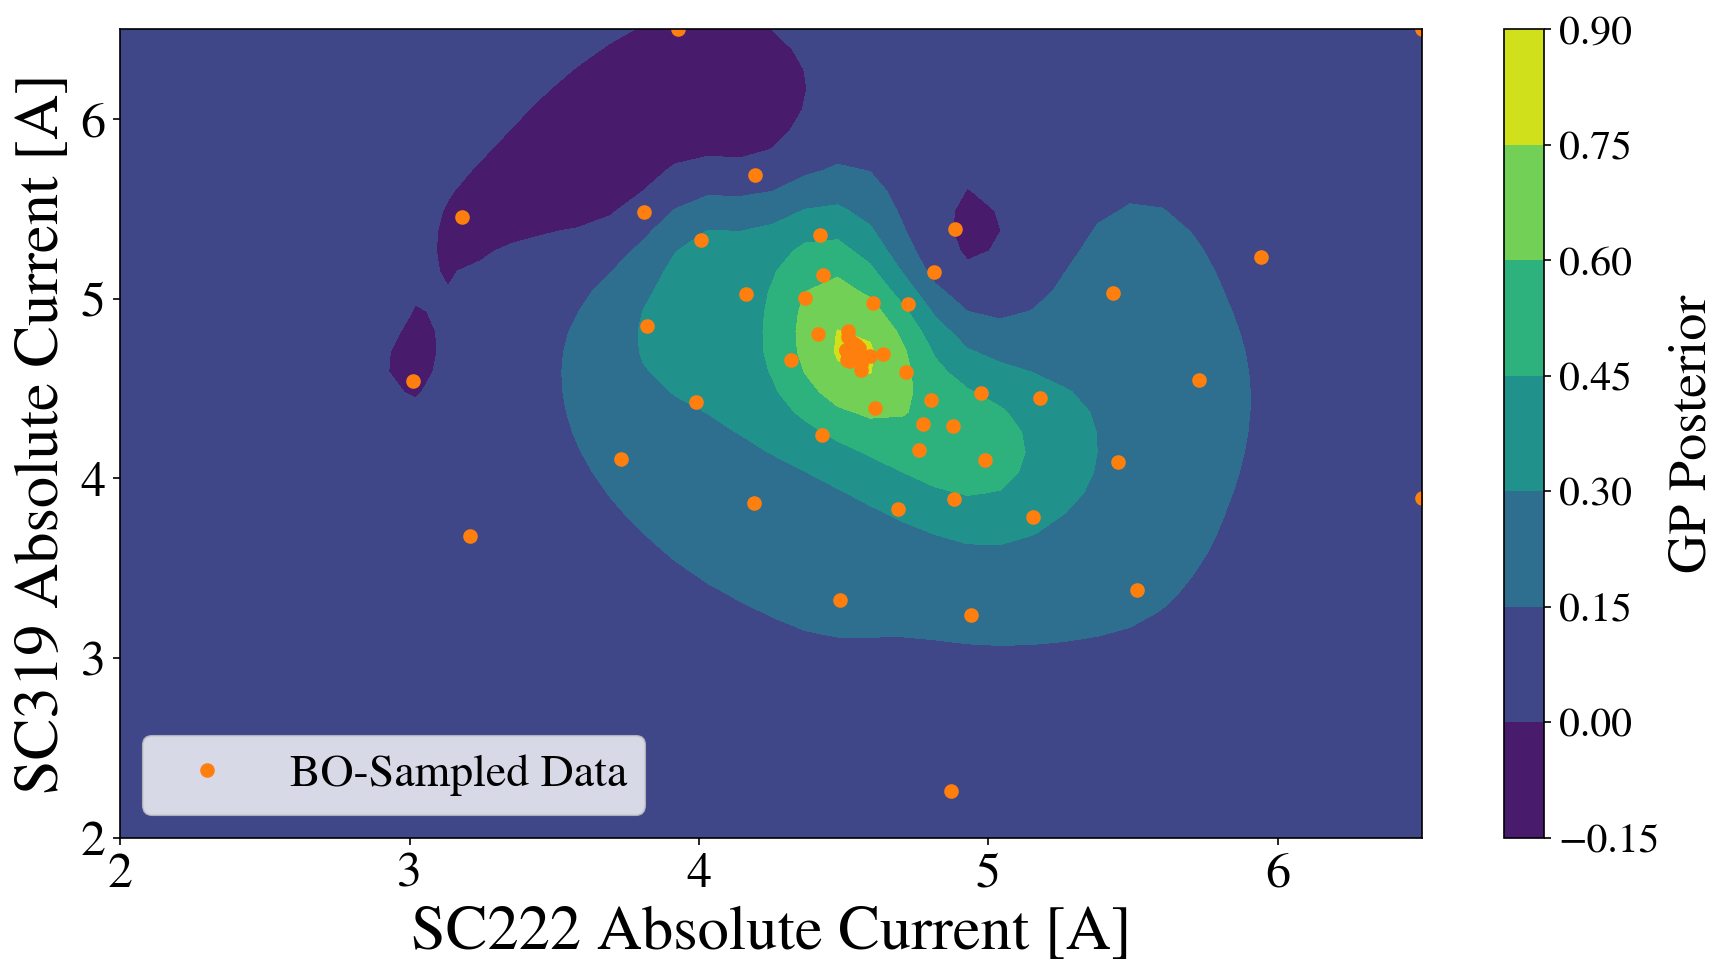
\includegraphics[width=\columnwidth]{chapter4/bo.png}
    \caption{Bayesian optimization of the compensation currents for $3Q_x$ transmission. The contour plot shows the Gaussian Process Posterior function trained by the sampled data (orange dots).}
    \label{fig:boRR}
\end{figure}

More advanced optimization algorithms can be used in order to fine-tune the best optimization currents in the compensation sextupoles. Figure \ref{fig:boRR} shows an instance were Bayesian optimization was used for this purpose. A summary of Bayesian optimization can be found in Ref. \cite{bayesian}. It is worth clarifying that the optimum currents from Fig. \ref{fig:boRR} differ from the ones in \ref{fig:neldermead} given that the first plot was generated from data taken in the 2022-2023 run and the other one from the 2021-2022 run. The tuning of the machine changes from year to year---even from week to week. The background contour plot of Fig. \ref{fig:boRR} corresponds to the Gaussian Process posterior trained from the Bayesian-guided sampling of the transmission through $3Q_x$. Ultimately, the cluster of points around the maximum show how the algorithm converged and found the best configuration to feed the sextupoles. These currents are close to the ones shown in Fig. \ref{fig:icomp_int}. Chapter \ref{sec:ch5} shows some studies done at the Proton-Synchrotron Booster (PSB) at CERN, where this optimization approach is fully embraced to compensate resonance lines.

\section{\label{sec:verify}Experimental Verification of Compensation}

\subsection{\label{sec:lossmaps}Dynamic Loss Maps}

One effective method for visualizing resonance compensation involves constructing dynamic loss maps. To generate these representations, specialized quadrupoles responsible for controlling the tune of the Recycler are gradually adjusted to map out the desired tune area. Throughout this process, the beam loss rate is meticulously measured and interpolated across the specified region. This is done in the horizontal and vertical direction. The initial horizontal scan is generated by maintaining a constant vertical tune while implementing a horizontal tune ramp ranging from $Q_x=25.47$ to $Q_x=25.31$. Subsequently, the vertical tune, initially set as \textit{constant} at $Q_y=24.47$, is adjusted incrementally to $Q_y=24.31$ in steps of 0.005, with intensity data recorded at each step. Conversely, for the vertical scan, the roles are reversed: the horizontal tune remains constant while a vertical tune ramp progresses from $Q_y=24.47$ to $Q_y=24.31$. Then, the \textit{constant} horizontal tune is varied from $Q_x=25.47$ to $Q_y=25.31$ in steps of 0.005. The resulting intensity data from both scans can be differentiated, normalized by the instantaneous intensity, and interpolated within a two-dimensional grid to construct plots akin to those depicted in Figs. \ref{fig:bare_nocomments} and \ref{fig:bare_comments}. Figure \ref{fig:bare_nocomments} demonstrates the initial machine scan without any compensation. If plotted alongside the theoretical positions of the lines as in Fig. \ref{fig:bare_comments}, the beam loss bands align with the resonance lines. 

Figure \ref{fig:bare_comments} illustrates the correspondence between the loss patterns and the theoretical positions of resonance lines. A slight deviation exists between the set tune and the actual tune due to calibration adjustments from the tune trombone program. However, despite this variance, the resonance line configuration within the loss pattern facilitates the visualization of each resonance's strength. Specifically, a higher normalized loss at a particular tune location indicates a stronger Resonance Driving Term (RDT) for the corresponding resonance line. Within Figs. \ref{fig:bare_nocomments} and \ref{fig:bare_comments}, third, fourth, and even traces of fifth-order resonance lines are discernible, with third-order resonance lines exhibiting the greatest prominence.

\begin{figure}[H]
    \centering
    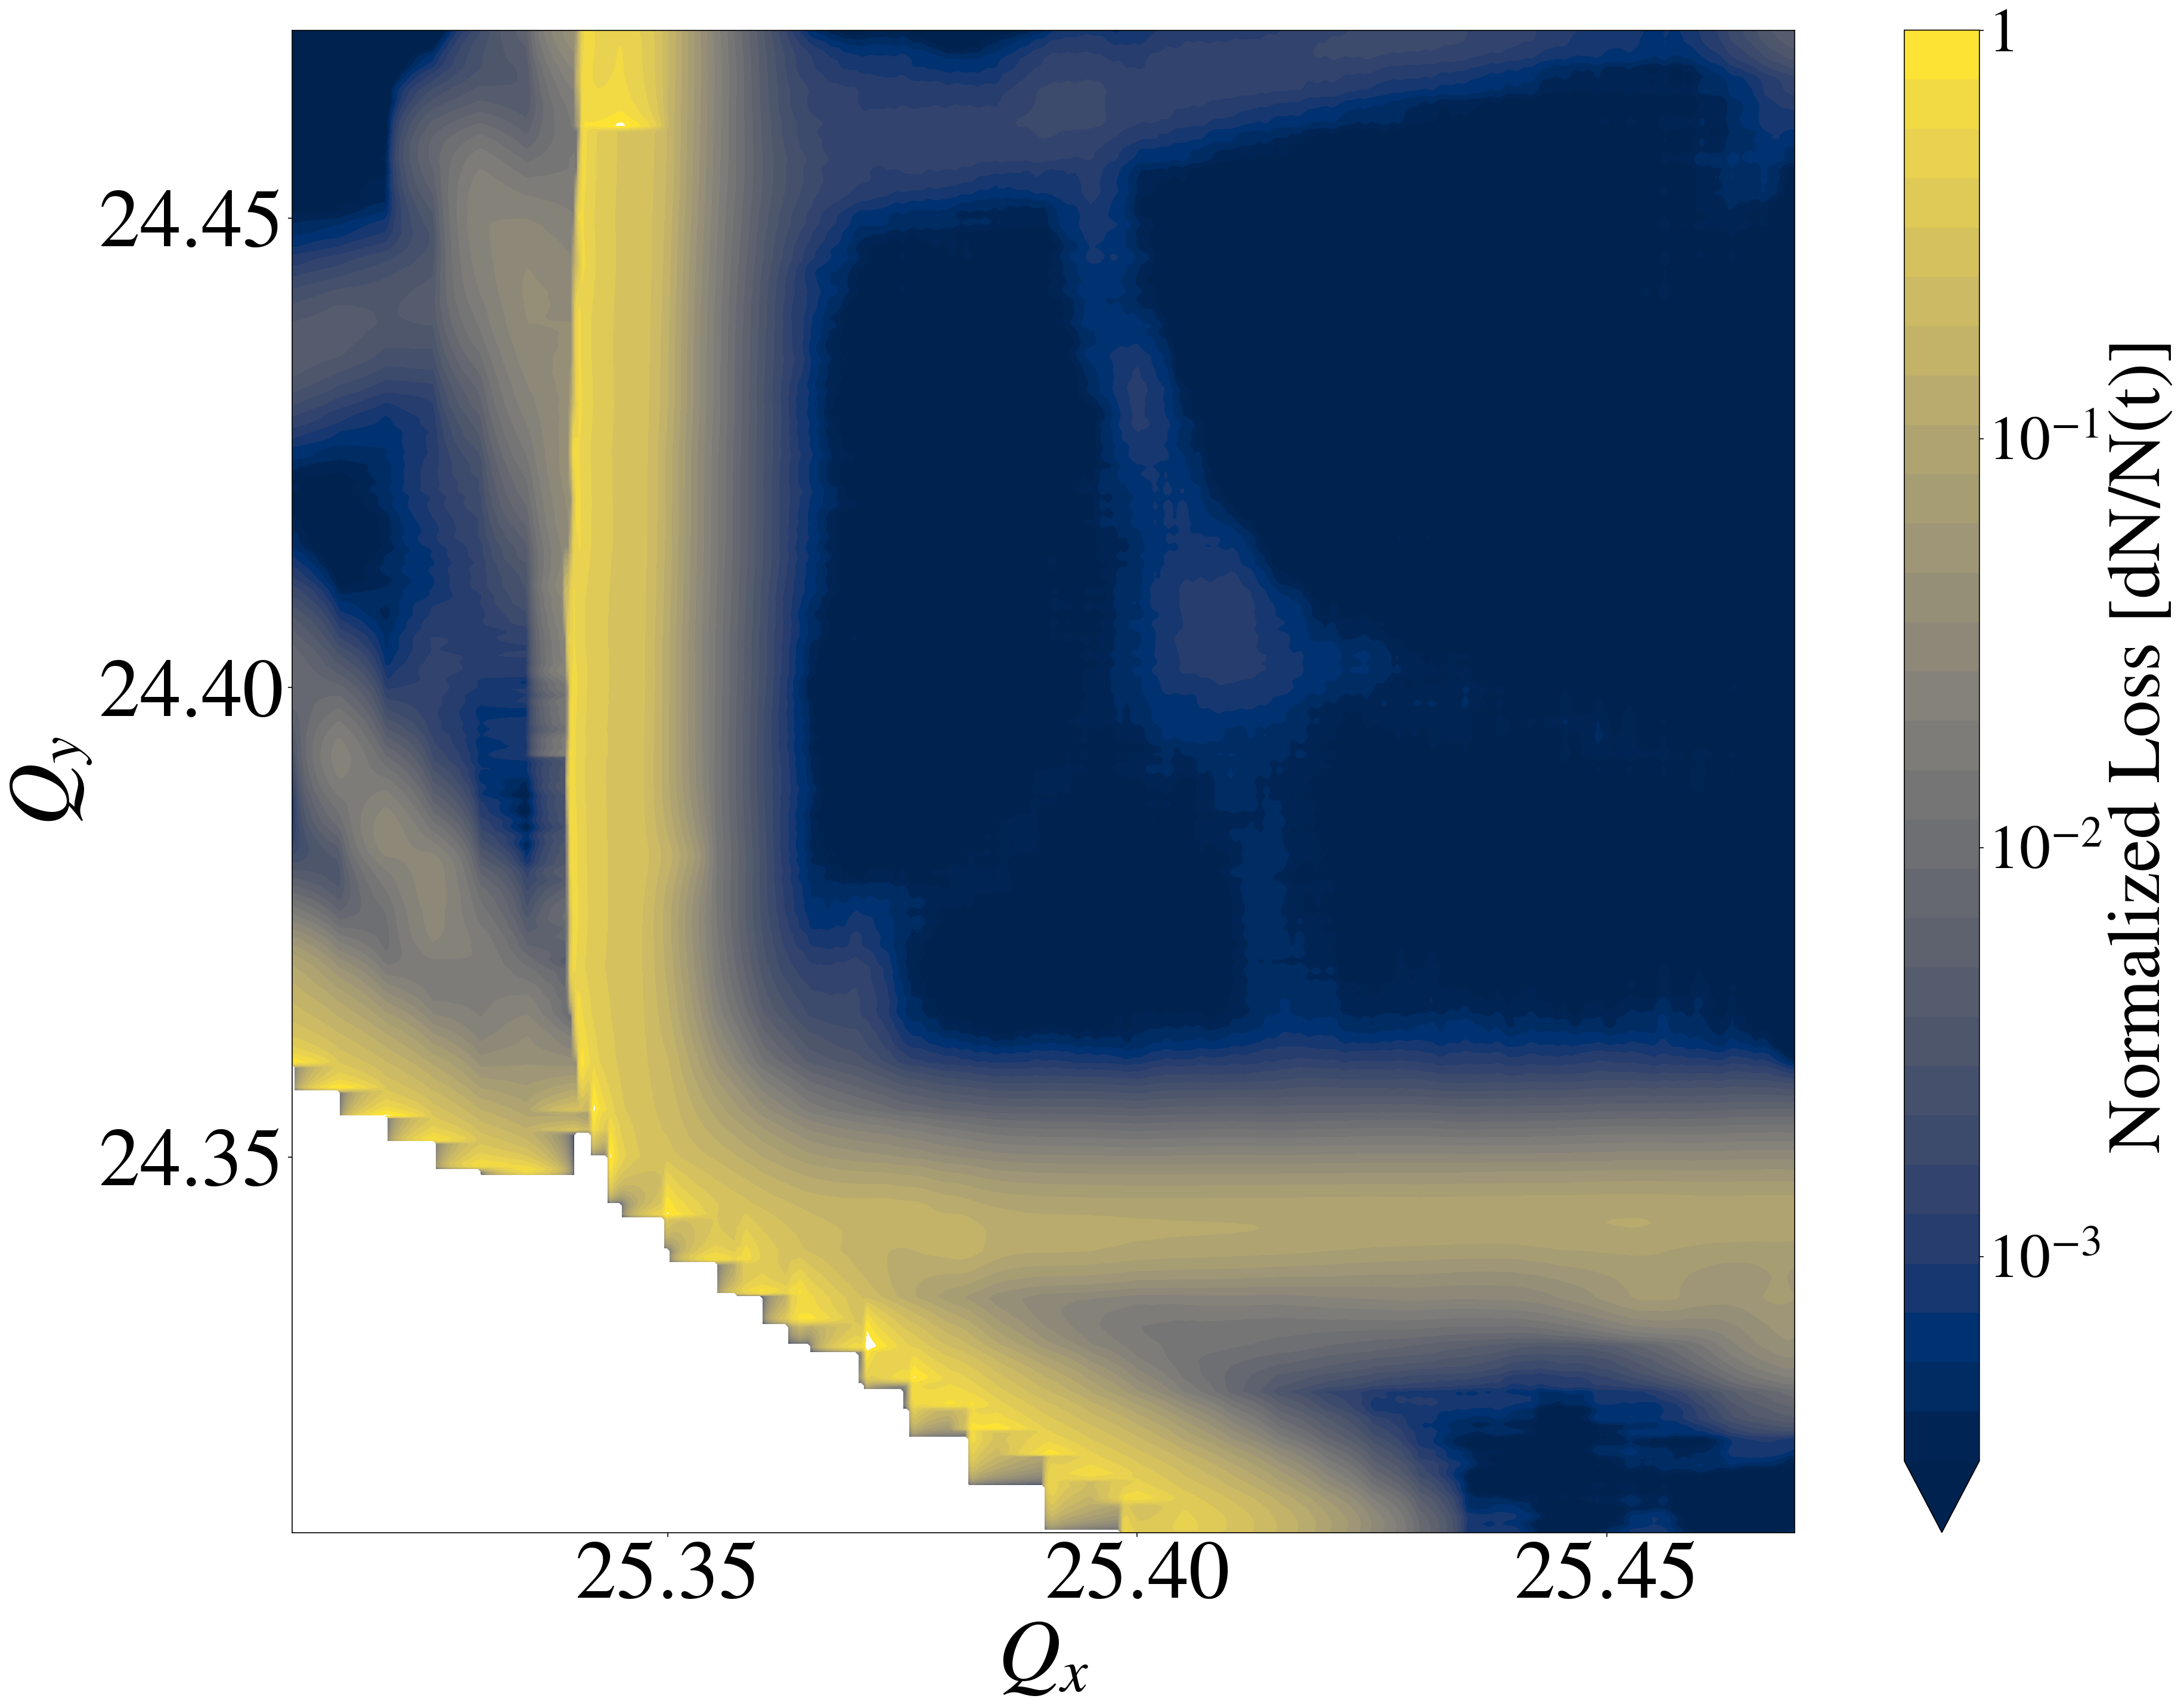
\includegraphics[width=\columnwidth]{chapter4/bare.png}
    \caption{Dynamic loss map from ramping the tunes with an interval of $\Delta Q_u=0.005$ in both directions. The directions of scan are from left to right and top to bottom. The results are superimposed in this plot.}
    \label{fig:bare_nocomments}
\end{figure}

Figure \ref{fig:lossmaps} depicts dynamic loss maps representing various configurations of the compensation sextupoles. Specifically, Fig. \ref{fig:sfig1} illustrates the loss map for the bare machine, where no compensation sextupoles are activated, while Fig. \ref{fig:sfig2} and Fig. \ref{fig:sfig3} demonstrate compensation for a single resonance line each. In the case of $3Q_x$ compensation, the four normal sextupoles are adjusted to the calculated compensation currents using the RDT response matrix method. Moreover, a comparison between Fig. \ref{fig:sfig2} and Fig. \ref{fig:sfig1} clearly indicates a reduction of normalized losses by two orders of magnitude at the $3Q_x$ line with compensation. This observation holds true for the $3Q_y$ compensation as well, as shown in Fig. \ref{fig:sfig3}.

\begin{figure}[H]
    \centering
    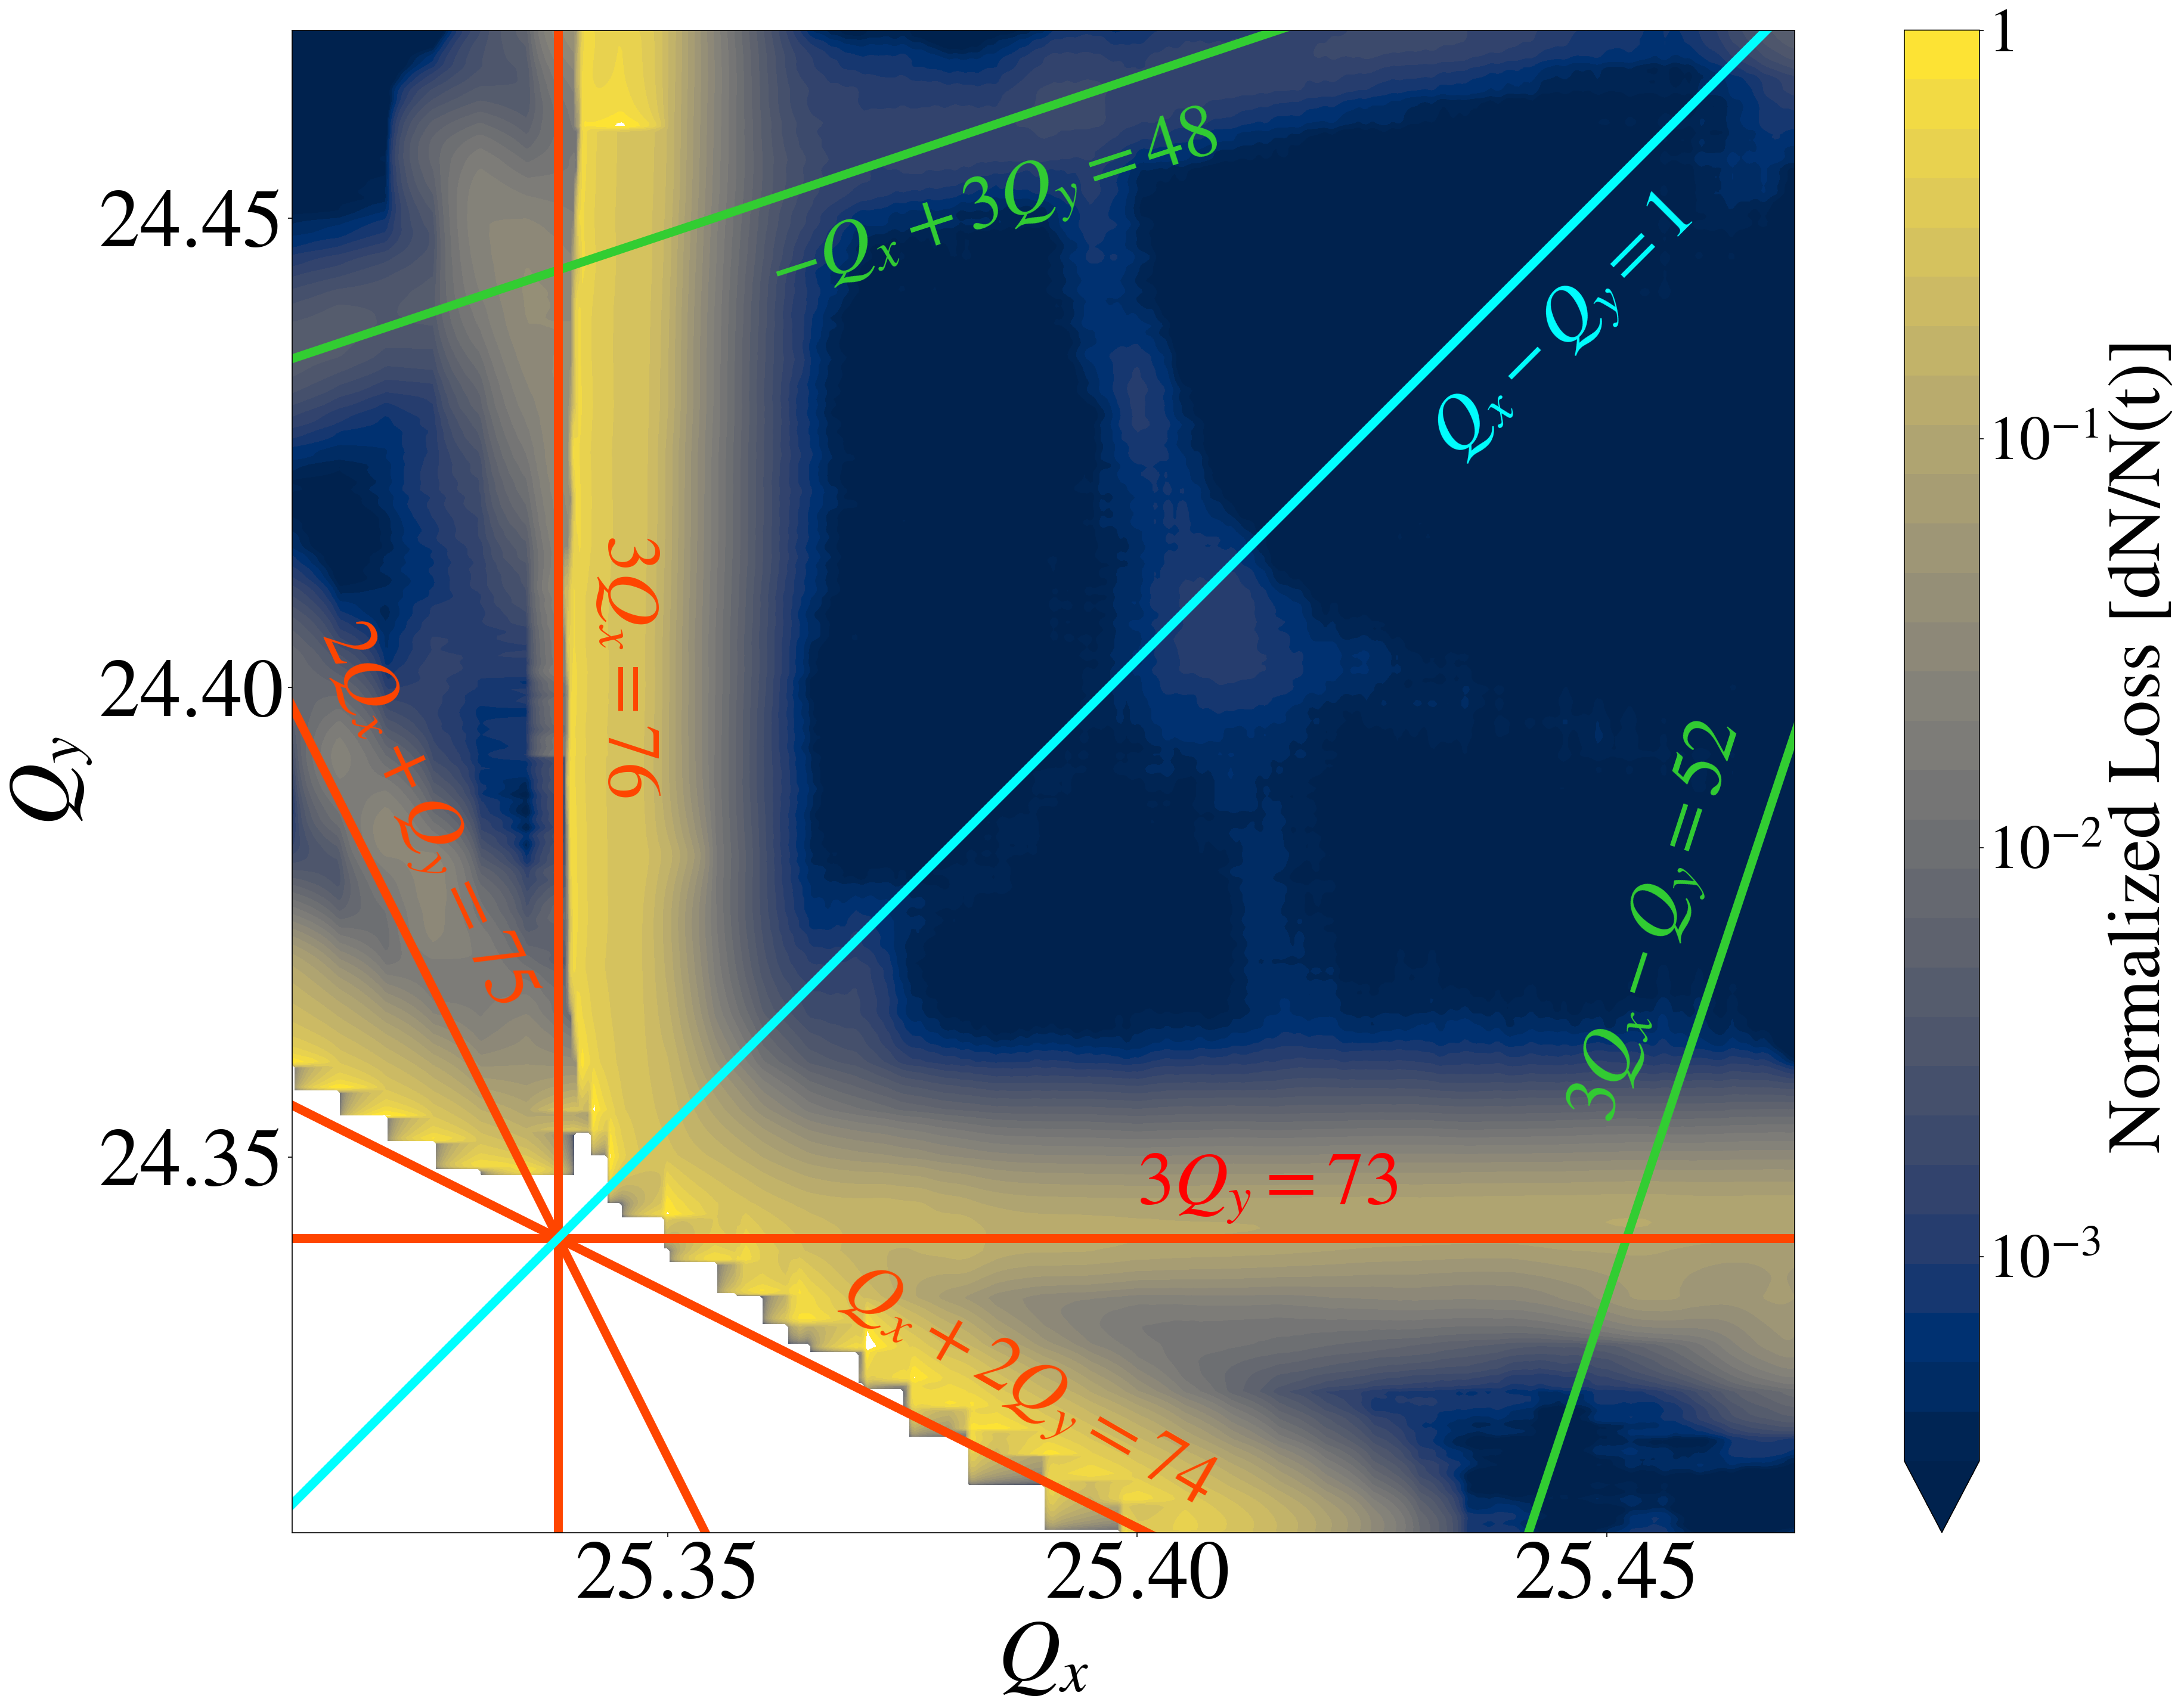
\includegraphics[width=\columnwidth]{chapter4/bare_comments.png}
    \caption{Dynamic loss map with the corresponding lines from Fig. \ref{fig:rrtd} drawn on top.}
    \label{fig:bare_comments}
\end{figure}

Figures \ref{fig:sfig4}, \ref{fig:sfig5}, and \ref{fig:sfig6} showcase the optimal configurations of compensation sextupoles designed to address multiple resonance lines simultaneously. It's important to note that while attempting to compensate for one or multiple resonance lines, there's a possibility that other resonance lines may strengthen. This is evident in the explicit case depicted in Fig. \ref{fig:sfig6}, where compensating for $3Q_y$ and $Q_x+2Q_y$ leads to the amplification of the $2Q_x+Q_y$ resonance. Such occurrences pose a limitation when aiming to compensate for more than two resonance lines, as the compensation currents tend to increase. There exists a constraint on the currents supplied to the compensation sextupoles. For instance, in compensating both normal sextupole lines, $3Q_x$ and $Q_x+2Q_y$, the required currents exceed the current limit. Ongoing efforts are focused on reducing the compensation currents in this specific scenario. Section \ref{sec:addsexts} summarizes some of these efforts, where additional sextupoles have been installed in order to decrease the currents that cancel out both the $h_{3000}$ and $h_{1020}$ RDTs.

Another notable detail evident in Figs. \ref{fig:sfig1}-\ref{fig:sfig6} is the presence of white areas within the loss maps, indicating regions where there was insufficient beam to accurately map out the losses. In certain configurations of the compensation sextupoles, the combined weakening of the third-order resonance lines occurs in a manner that leaves some beam remaining beyond these lines. It could be argued that conducting two additional scans, injecting from the left and bottom, could effectively map out these inaccessible regions. Such an enhancement could be considered as a future upgrade to these dynamic loss maps. Ultimately, all the plots presented in Fig. \ref{fig:lossmaps} demonstrate various potential configurations that open up regions of tune space for utilization during operations, enabling the accommodation of high-intensity beams.

\newpage
\begin{figure}[H]

    \centering
    \begin{subfigure}{.49\textwidth}
      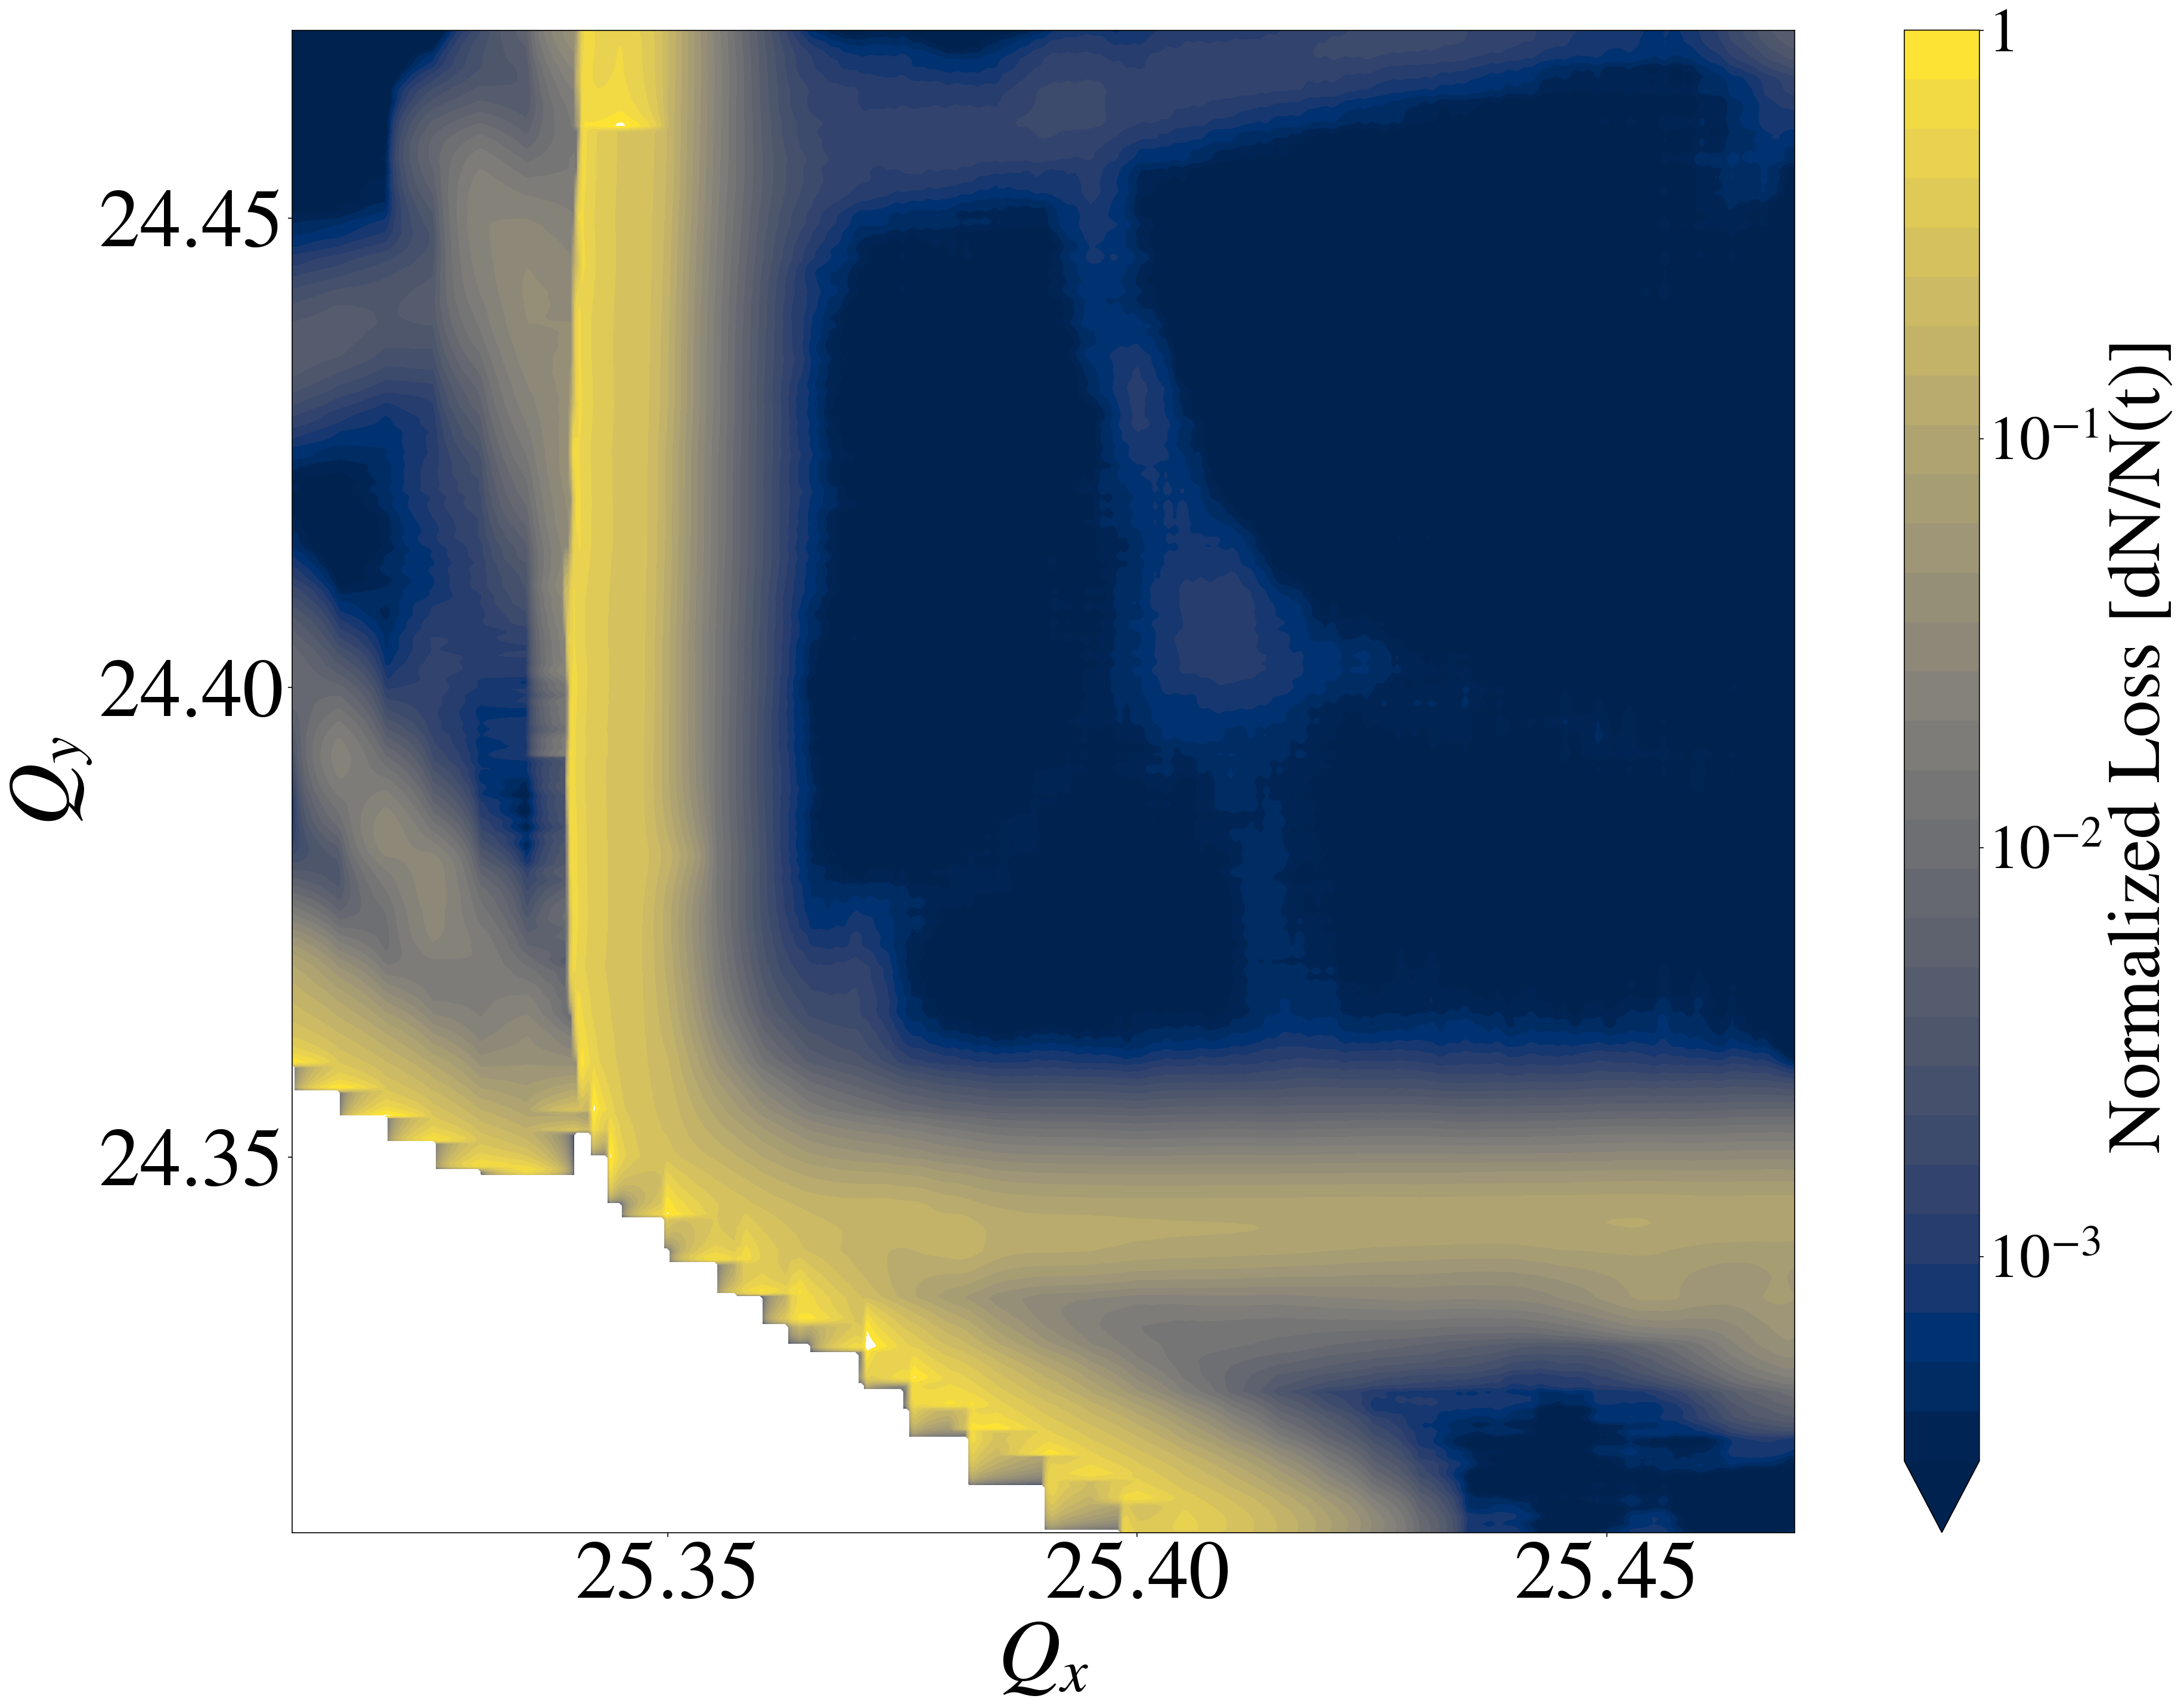
\includegraphics[width=0.98\linewidth]{chapter4/bare.png}
      \caption{Bare machine}
      \label{fig:sfig1}
    \end{subfigure}%
    \hfill
    \begin{subfigure}{.49\textwidth}
      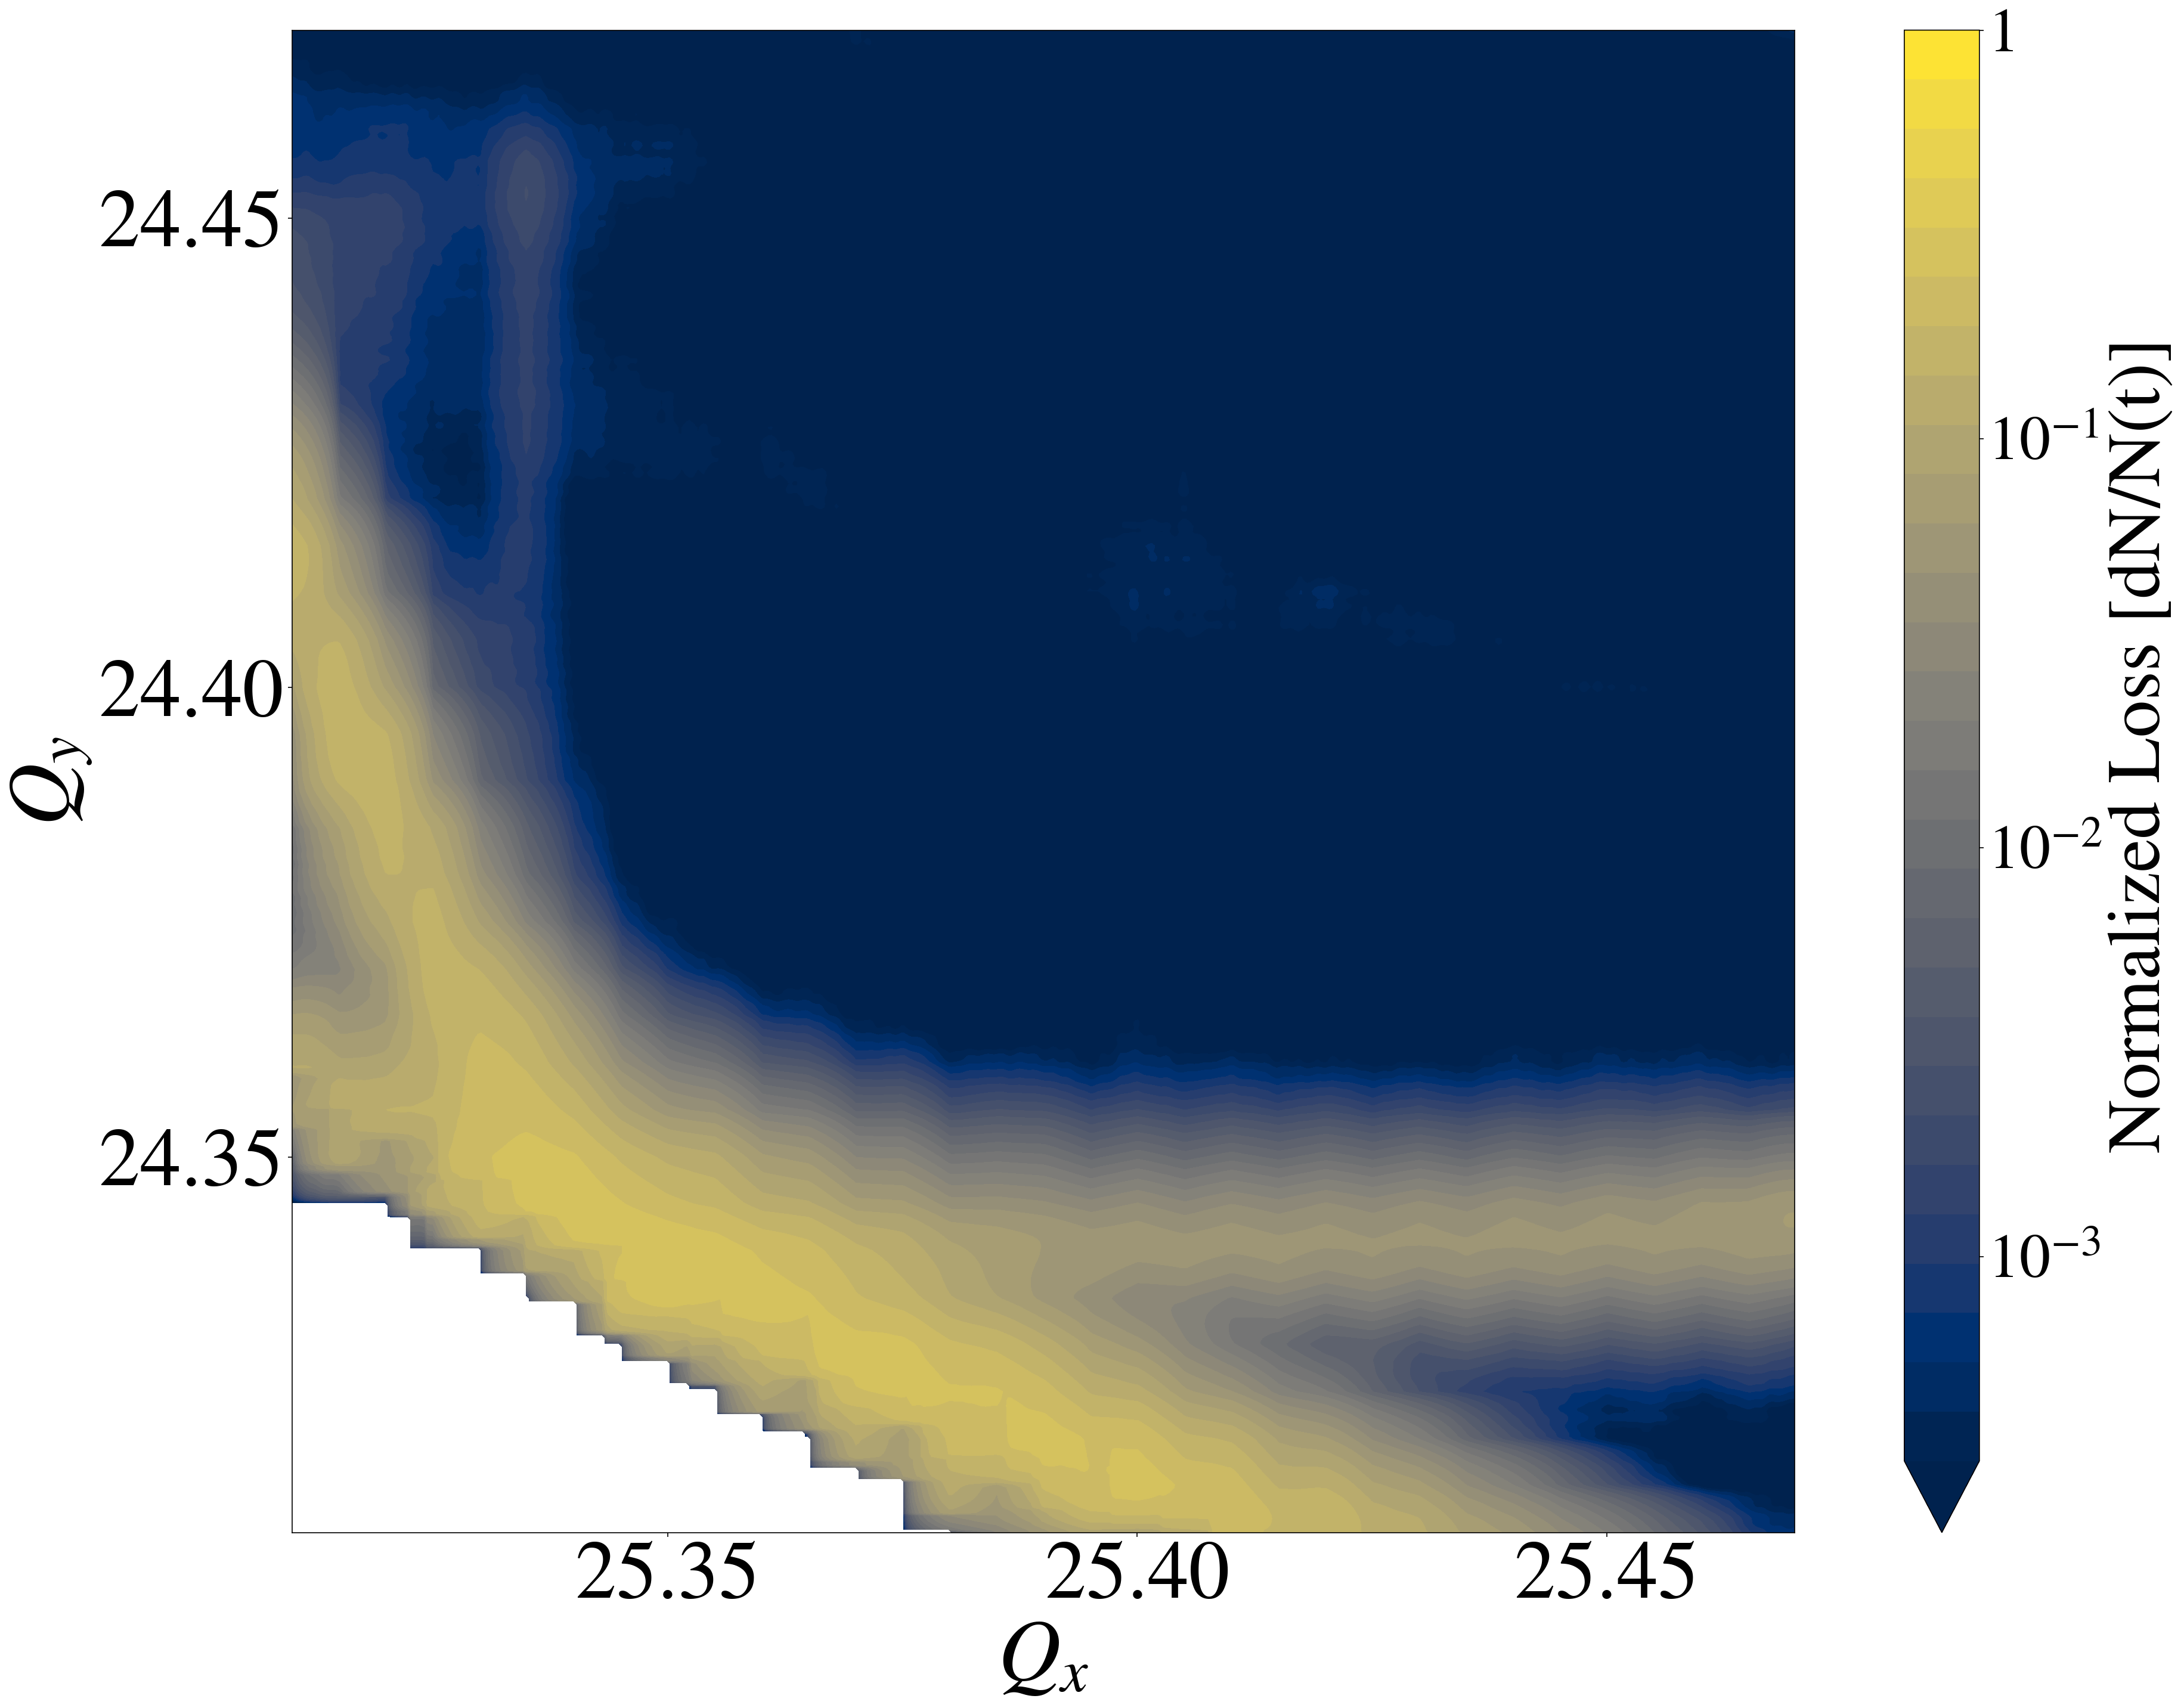
\includegraphics[width=0.98\linewidth]{chapter4/3qx.png}
      \caption{$3Q_x$ Compensation}
      \label{fig:sfig2}
    \end{subfigure}
    \hfill
    \begin{subfigure}{.49\textwidth}
      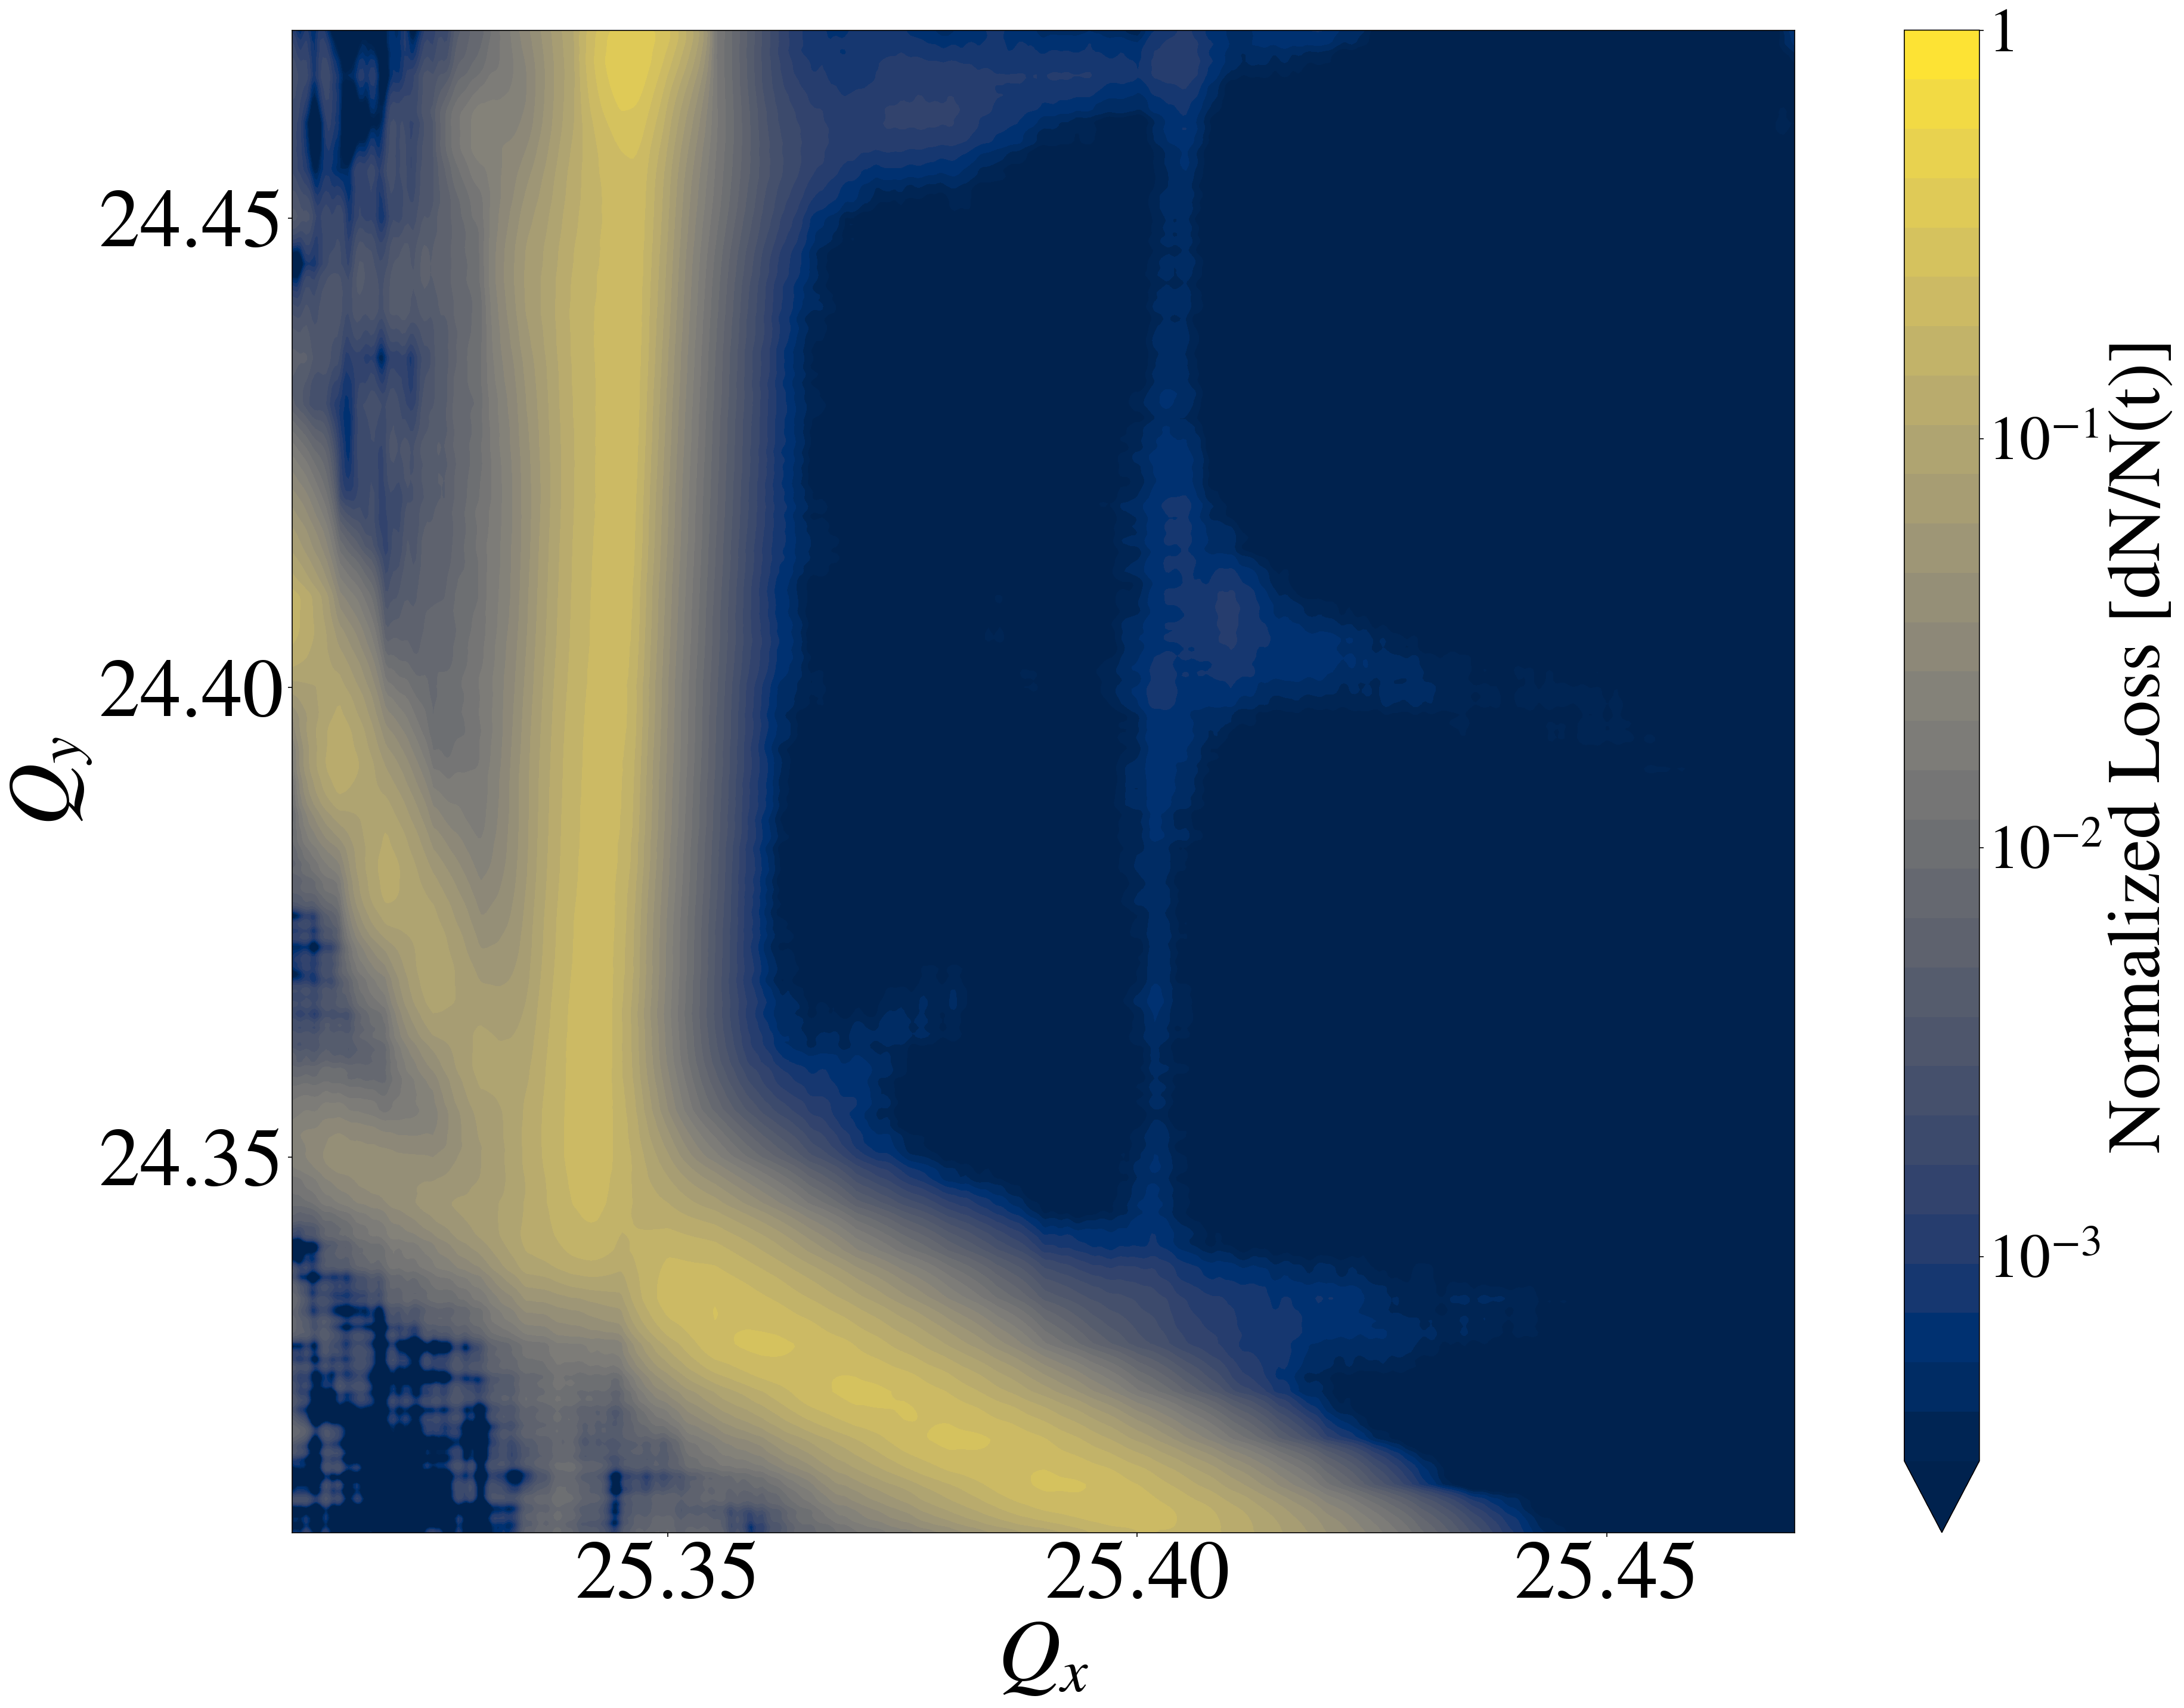
\includegraphics[width=0.98\linewidth]{chapter4/3qy.png}
      \caption{$3Q_y$ Compensation}
      \label{fig:sfig3}
    \end{subfigure}
    \hfill
    \begin{subfigure}{.49\textwidth}
      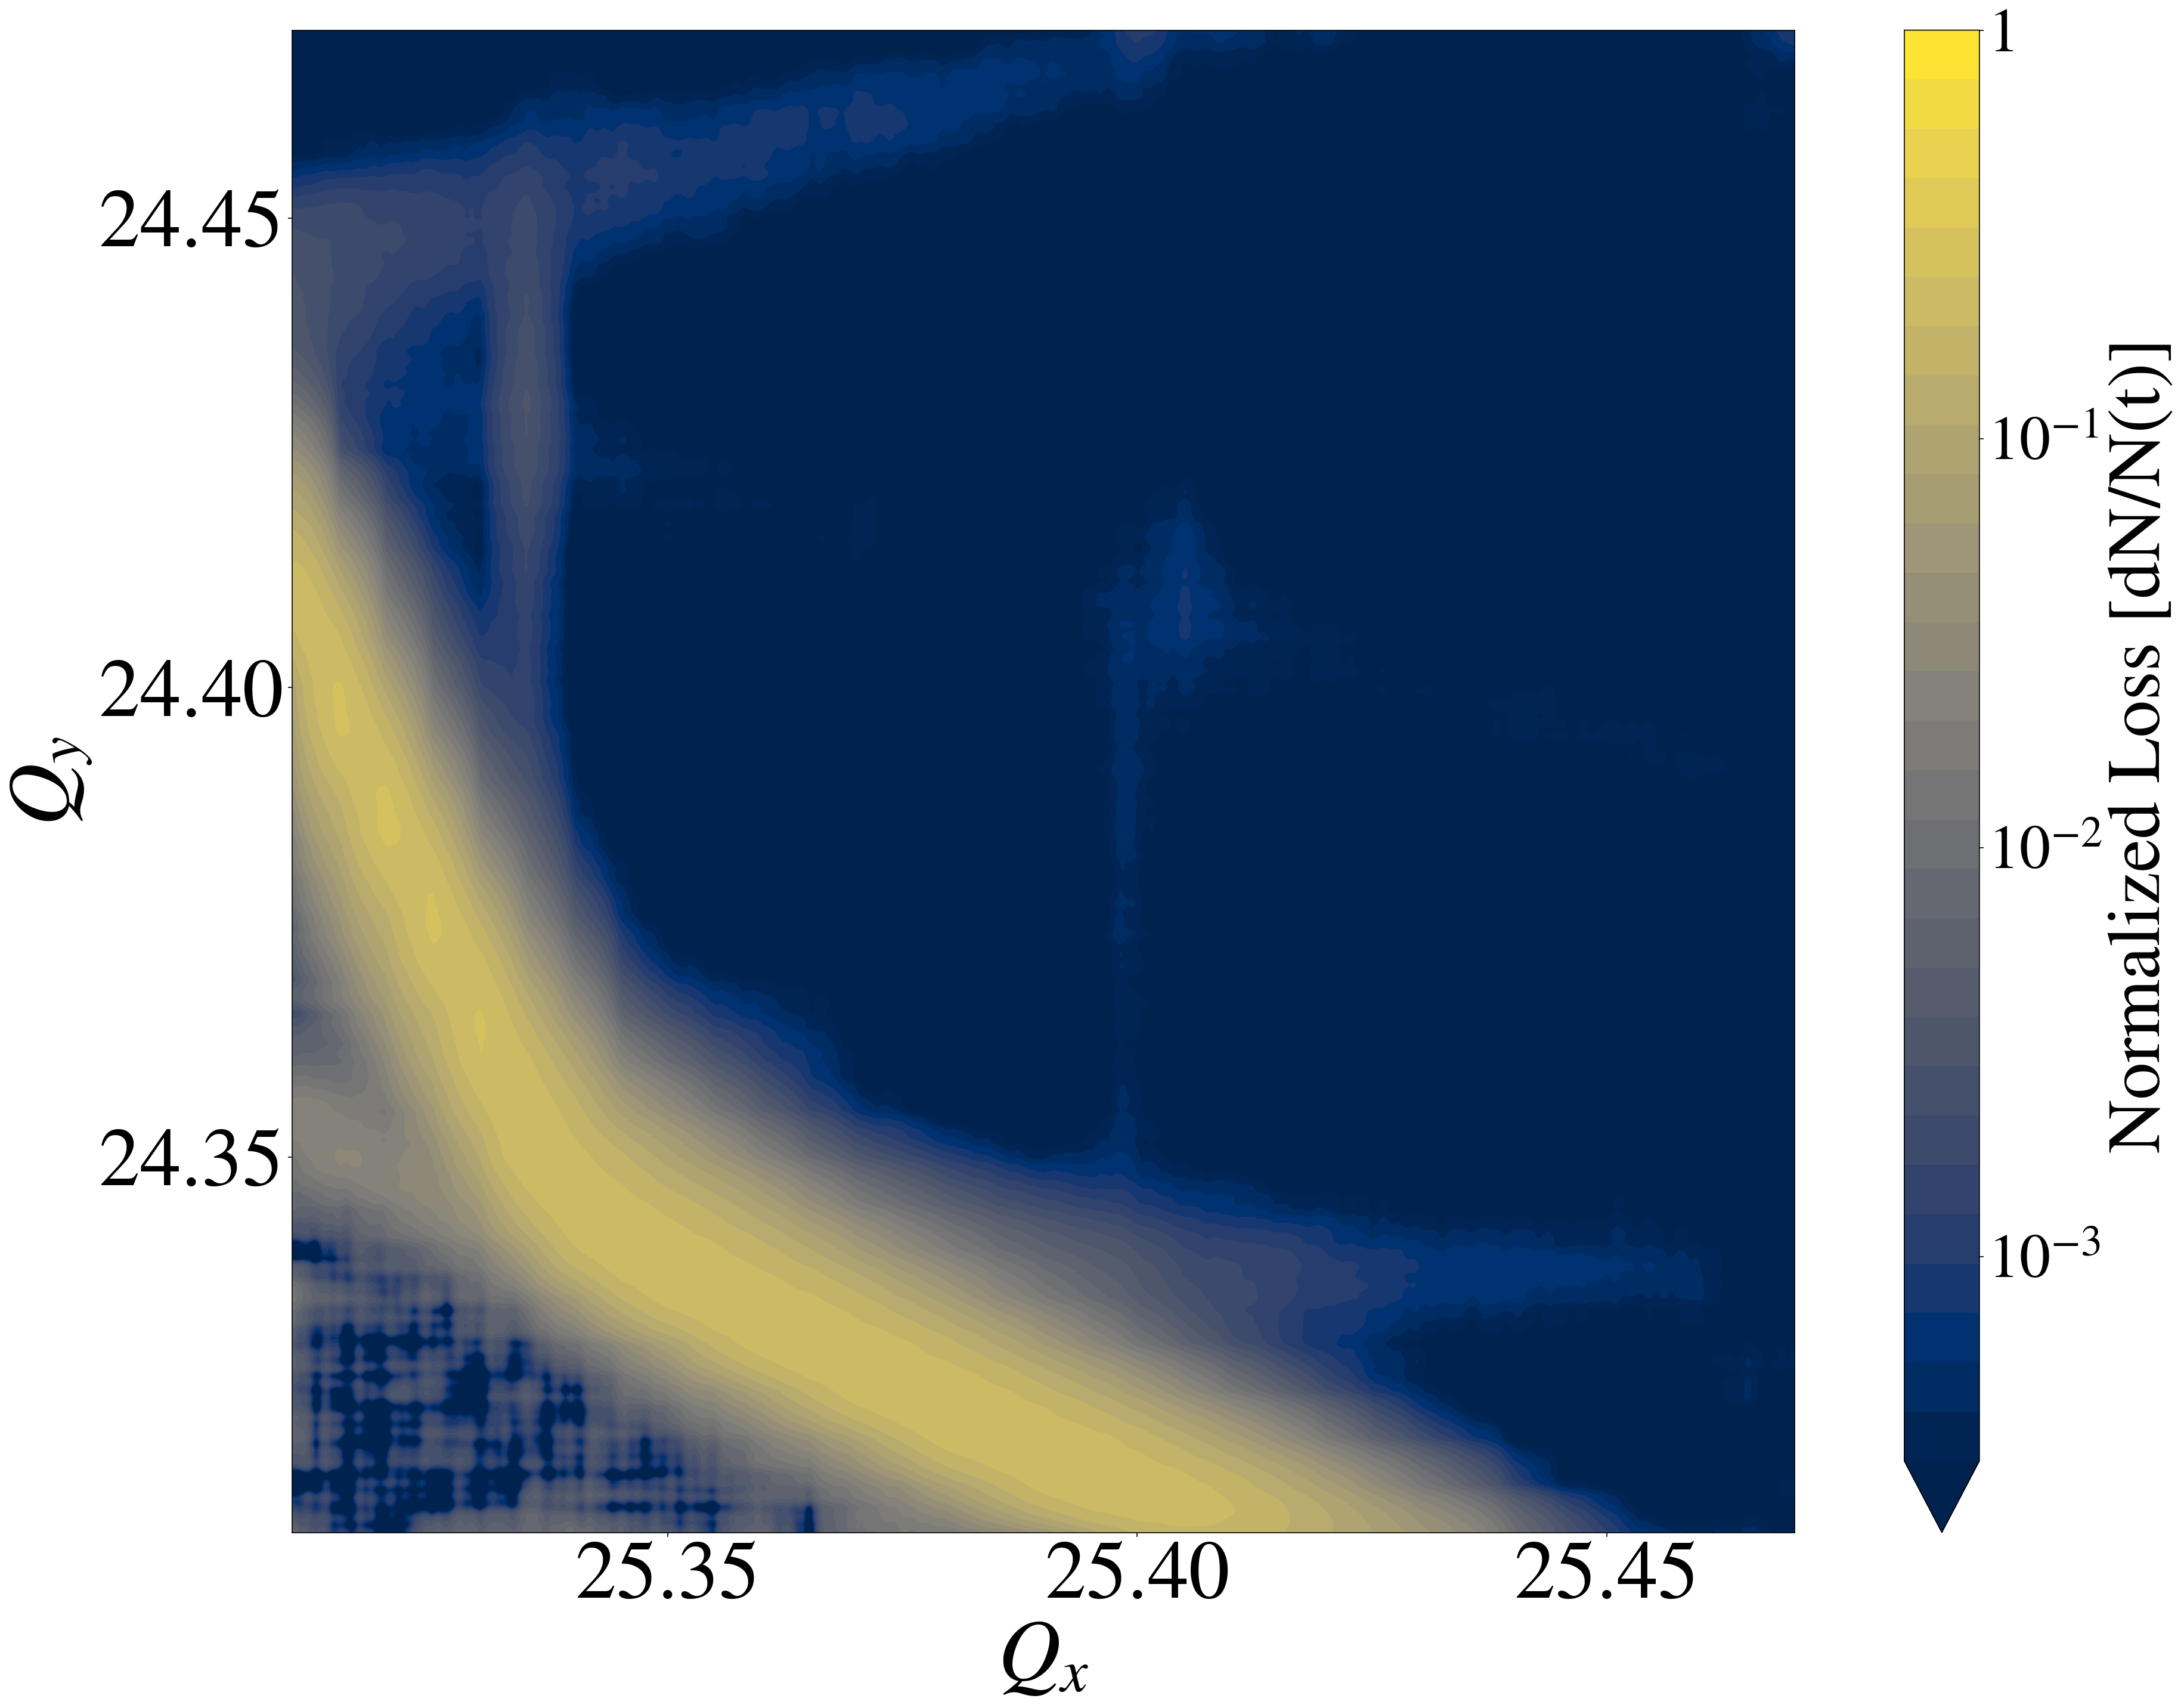
\includegraphics[width=0.98\linewidth]{chapter4/3qx_3qy.png}
      \caption{$3Q_x$ and $3Q_y$ Compensation}
      \label{fig:sfig4}
    \end{subfigure}%
    \hfill
    \begin{subfigure}{.49\textwidth}
      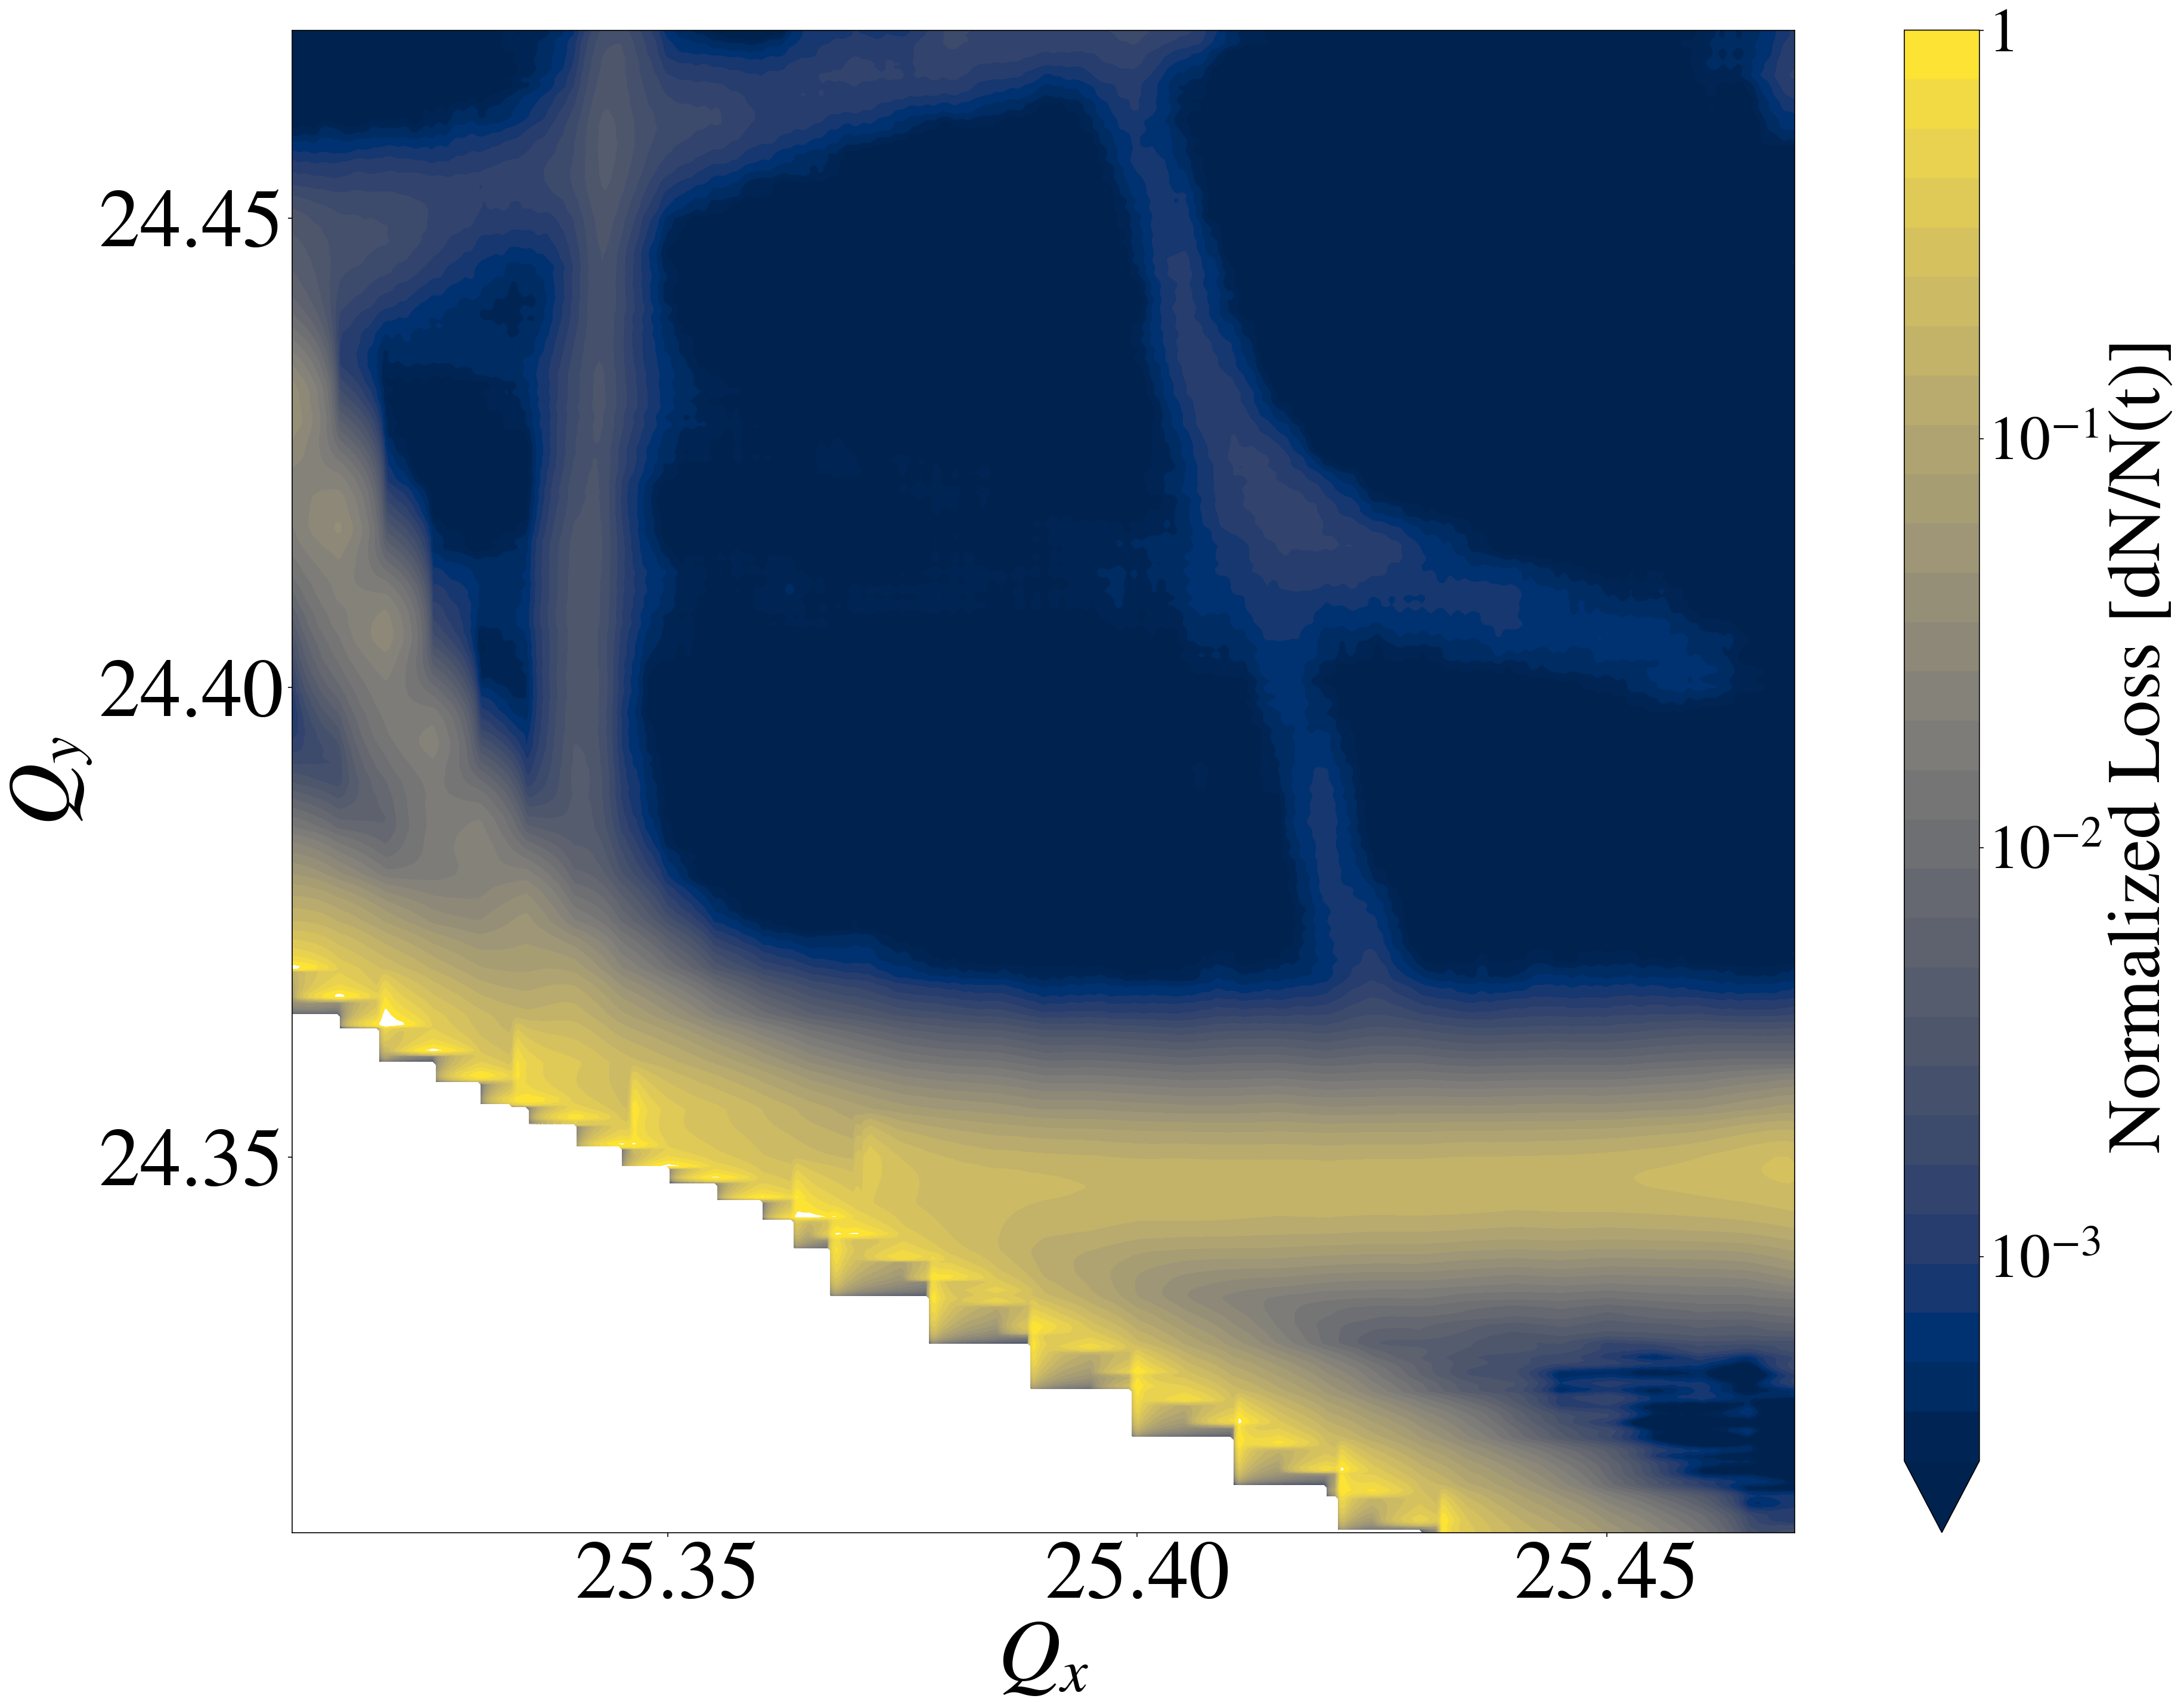
\includegraphics[width=0.98\linewidth]{chapter4/3qx_2qxqy.png}
      \caption{$3Q_x$ and $2Q_x+Q_y$ Compensation}
      \label{fig:sfig5}
    \end{subfigure}
    \hfill
    \begin{subfigure}{.49\textwidth}
      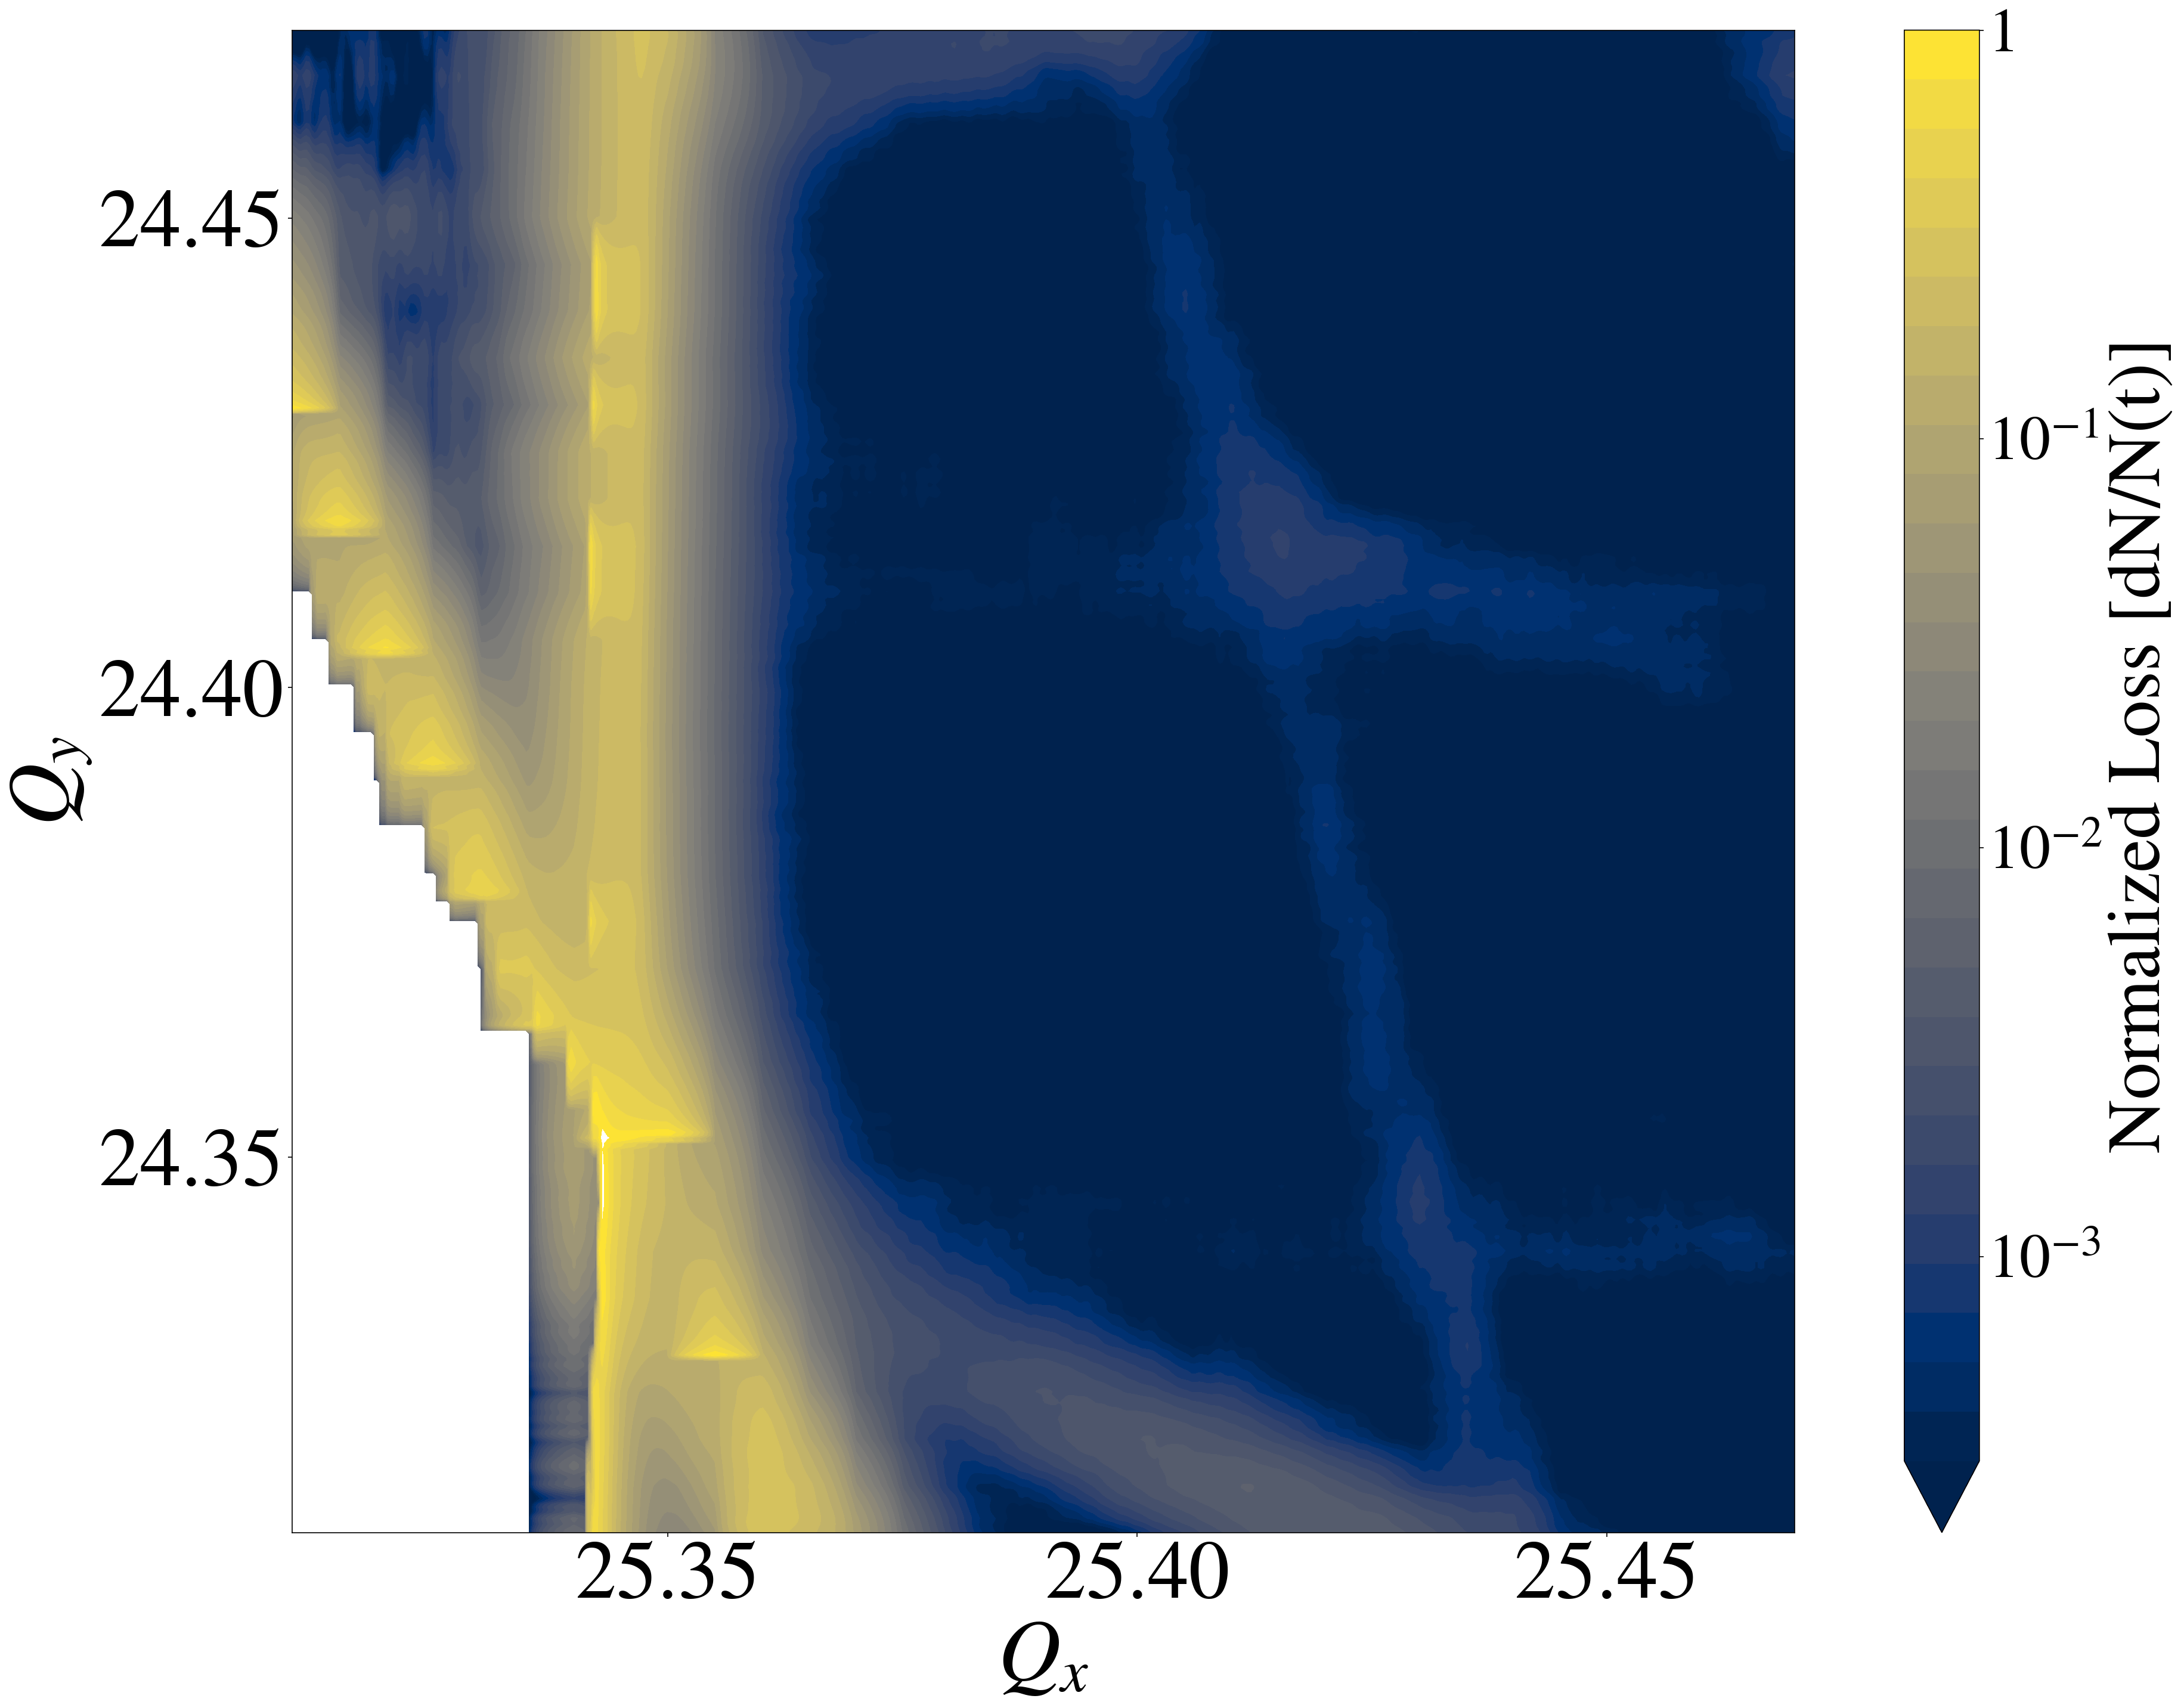
\includegraphics[width=0.98\linewidth]{chapter4/3qy_qx2qy.png}
      \caption{$3Q_y$ and $Q_x+2Q_y$ Compensation}
      \label{fig:sfig6}
    \end{subfigure}
    
    \caption{Dynamic loss maps for several configurations of compensation sextupoles}
    \label{fig:lossmaps}
    \end{figure} 
\newpage


\subsection{Static Tune Scans}

Another method for visualizing resonance compensation involves static tune scans. While the loss maps detailed earlier illustrate the dynamic crossing of resonances, an alternative method entails setting the tune to a specific value and assessing the beam survival ratio alongside the beam size over a defined time interval. This time interval was around 0.8 seconds equivalent to around 72800 turns. The beam survival ratio was calculated from the beam intensity data captured from the DC Current Transformer (DCCT). The beam size is quantified using the Ion Profile Monitor System (IPM) within the ring, as introduced in Sec. \ref{sec:diagnostic}.

\begin{figure}[H]
    \centering
    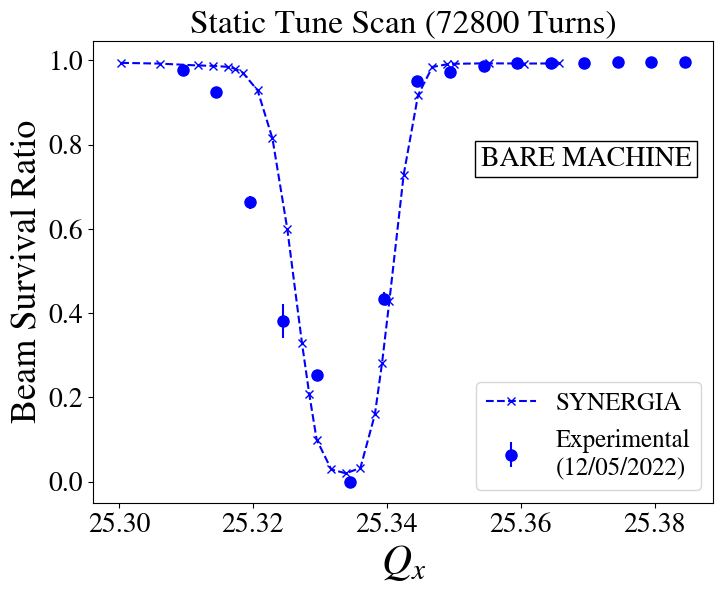
\includegraphics[width=\columnwidth]{chapter4/static2turns.png}
    \caption{Static tune scan for bare machine with comparisons between experimental data and SYNERGIA simulations at a low intensity of 0.5e10 particles per bunch (2 Booster Turns of equivalent intensity).}
    \label{fig:static2}
\end{figure}

Figure \ref{fig:static2} shows a static tune scan only including beam survival ratio data. This plot includes data from experiments and data from SYNERGIA simulations done with no space charge. Given that these experiments were done at low intensities, no space-charge simulator was utilized. The simulations were done for 72800 turns, and the experimental data was partitioned to only this equivalent time window. Figure \ref{fig:static2} shows the resonance stop band corresponding to $3Q_x$ resonance. Effectively, no beam survives when beam is parked on top of the resonance line. There is a good agreement between the simulations and the experimental data. This hints at the fact that the model is capturing the sextupole component around the ring, even if it is not perfect. Nevertheless, left of the resonance the experimental starts deviating from the model, given that the Recycler Ring is not optimized to run in this region.

% \begin{figure}[H]
%     \centering
%     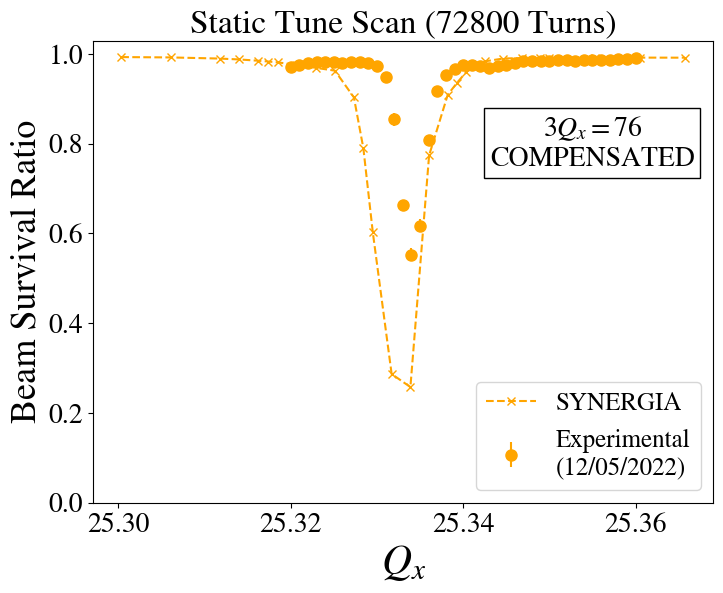
\includegraphics[width=\columnwidth]{chapter4/static2turns_comp.png}
%     \caption{Plot for static tune scan for machine with $3Q_x$ compensation including comparison between experimental data and SYNERGIA simulations.}
%     \label{fig:static2_comp}
% \end{figure}

\begin{figure}[H]
    \centering
    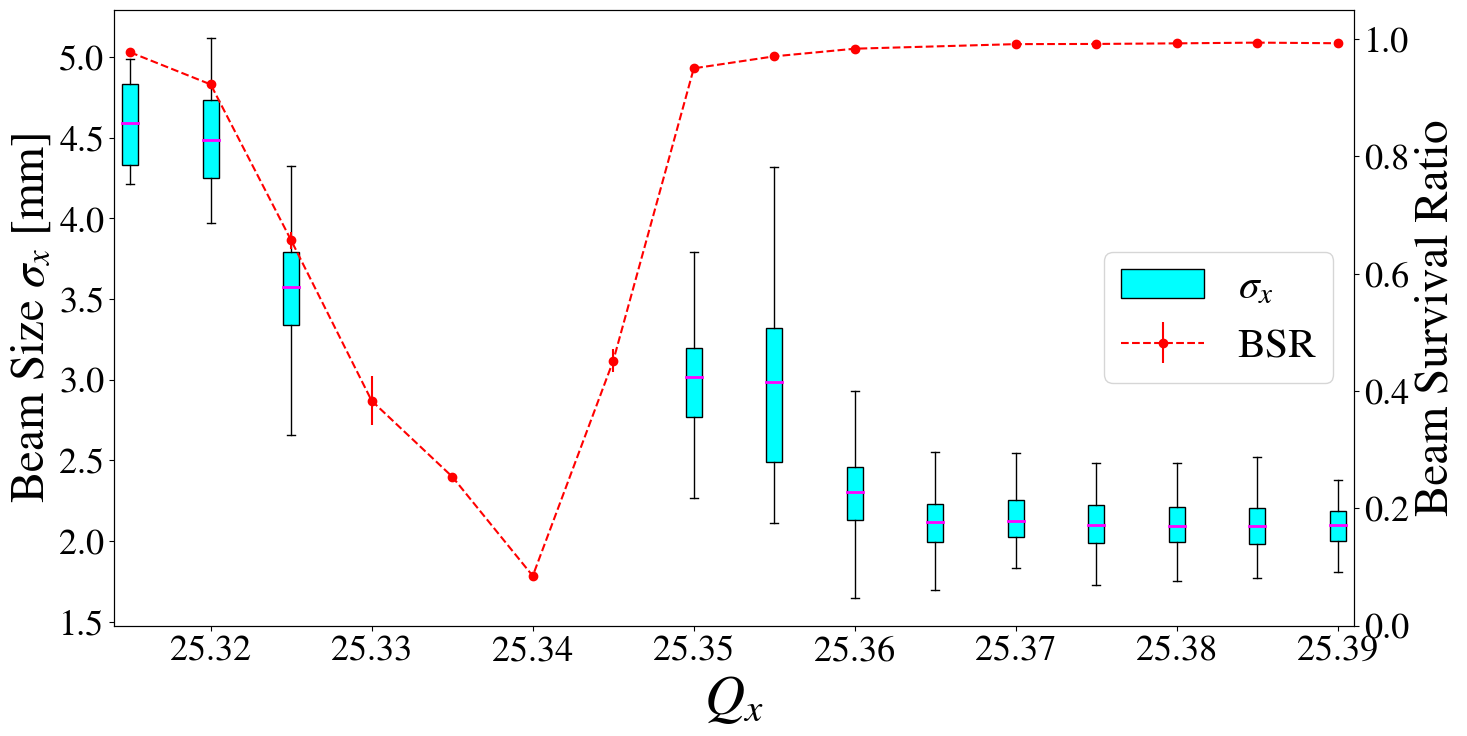
\includegraphics[width=\columnwidth]{chapter4/static2turns_ipm.png}
    \caption{Static tune scan with beam survival ratio and IPM data box plots for bare machine at 2 Booster Turns of equivalent intensity.}
    \label{fig:static2_ipm}
\end{figure}

\begin{figure}[H]
    \centering
    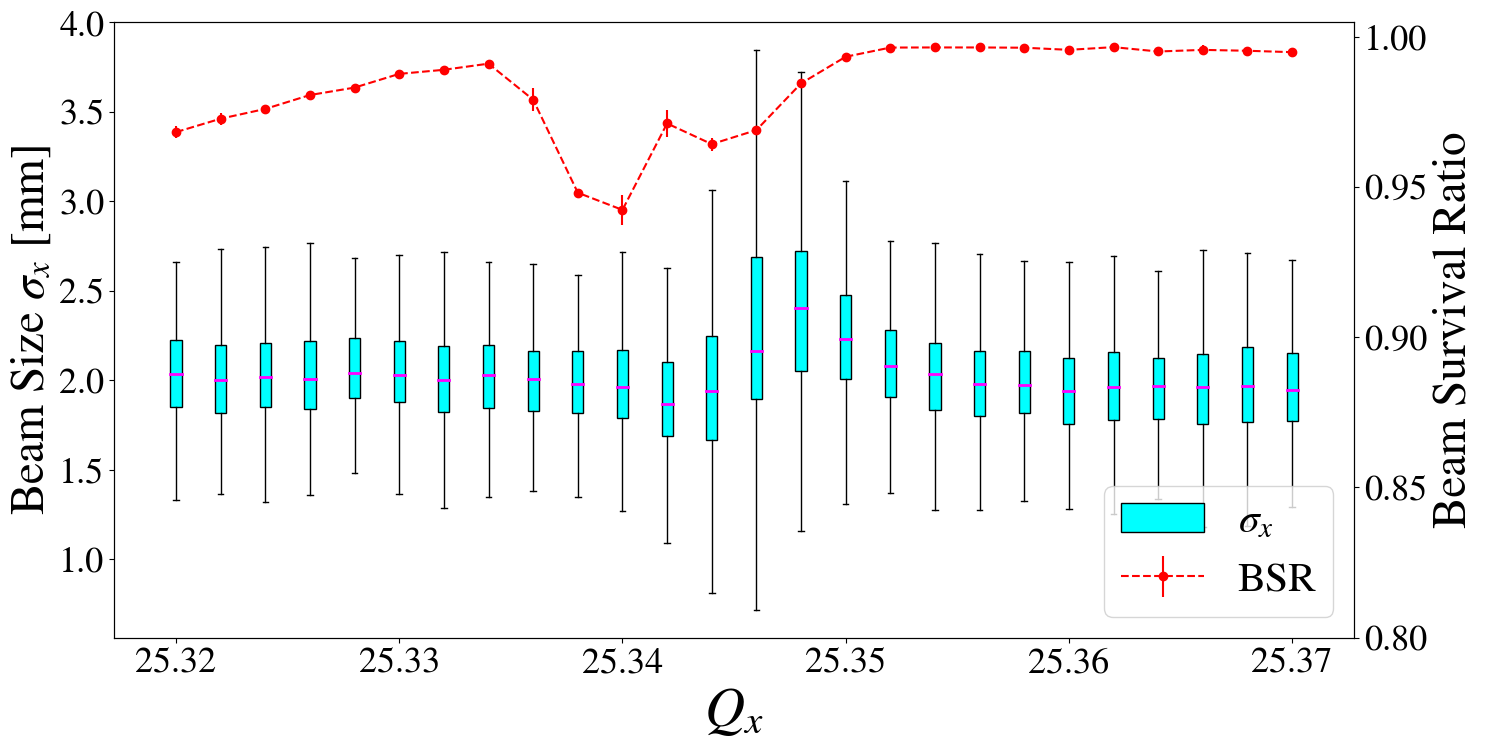
\includegraphics[width=\columnwidth]{chapter4/static2turns_comp_ipm_dampersOFF.png}
    \caption{Static tune scan with beam survival ratio and IPM data box plots for machine with $3Q_x$ compensation at 2 Booster Turns of equivalent intensity.}
    \label{fig:static2_ipm_comp}
\end{figure}

\section{Additional Sextupoles for Resonance Compensation}
\label{sec:addsexts}

As mentioned before in the discussion of Figs. \ref{fig:h3000_3qxcomp}, \ref{fig:h1020_3qxcomp} and \ref{fig:lossmaps}, the currents in the compensation sextupoles that cancel out the $h_{3000}$ and $h_{1020}$ RDTs are too large. This section explores the idea of introducing two additional normal compensation sextupoles in order to bring down the $K_2$ coefficients that cancel out both of this RDTs---effectively, bring down the currents in all the sextupoles. Therefore, this section looks at finding the right location for these two new sextupoles. The introduction of two new sextupoles implies that the RDT equation from Eq. \ref{eq:model1} is modified and this reads:
\begin{equation}
    \begin{bmatrix}
        -|h_{3000}| \cos \psi_{3000} \\
        -|h_{3000}| \sin \psi_{3000} \\
        -|h_{1020}| \cos \psi_{1020} \\
        -|h_{1020}| \sin \psi_{1020} \\
        \end{bmatrix}_{(Bare)}
         =
        \boldsymbol{M_A}
        \begin{bmatrix}
        K_2^{(sc220)} \\
        K_2^{(sc222)}\\
        K_2^{(sc319)} \\
        K_2^{(sc321)}\\
        K_2^{(1)} \\
        K_2^{(2)}\\
        \end{bmatrix}.
        \label{eq:systemadd}
\end{equation}
In this case, the response matrix gets appended two new columns with the RDT sensitivity of the two new sextupoles. This reads:
\begin{equation}
    \boldsymbol{M_A} =
\begin{bmatrix}
\begin{pmatrix}  \boldsymbol{M} \\ \end{pmatrix} 
& \begin{matrix} \frac{1}{48} l_{sc} \: \beta^{3/2}_{x(1)} \: \cos 3\phi_{x(1)} & \frac{1}{48} l_{sc} \: \beta^{3/2}_{x(2)} \: \cos 3\phi_{x(2)} \\ 
 \frac{1}{48} l_{sc} \: \beta^{3/2}_{x(1)} \: \sin 3\phi_{x(1)} & \frac{1}{48} l_{sc} \: \beta^{3/2}_{x(2)} \: \sin 3\phi_{x(2)}  \\ 
 \frac{1}{16} l_{sc} \: \beta^{1/2}_{x(1)} \beta_{y(1)} \: \cos \left( \phi_{x(1)} + 2\phi_{y(1)} \right) &  \frac{1}{16} l_{sc} \: \beta^{1/2}_{x(2)} \beta_{y(2)} \: \cos \left( \phi_{x(2)} + 2\phi_{y(2)} \right)\\ 
 \frac{1}{16} l_{sc} \: \beta^{1/2}_{x(1)} \beta_{y(1)} \: \sin \left( \phi_{x(1)} + 2\phi_{y(1)} \right) &  \frac{1}{16} l_{sc} \: \beta^{1/2}_{x(2)} \beta_{y(2)} \: \sin \left( \phi_{x(2)} + 2\phi_{y(2)} \right)\\  
\end{matrix}\\
\end{bmatrix},
\end{equation}
where the beta functions and phases are evaluated at a lattice location still yet to be determined. The original matrix $\boldsymbol{M}$ is the one defined from Eq. \ref{eq:model2}. 

The first step was to minimize the function
\begin{equation}
    \label{eq:fmax}
    f\left(\beta_{x(i)},\beta_{y(i)}, \phi_{x(i)}, \phi_{y(i)}\right) = \max \left(
    \begin{bmatrix}
    K_2^{(sc220)} \\
    K_2^{(sc222)}\\
    K_2^{(sc319)} \\
    K_2^{(sc321)}\\
    K_2^{(1)} \\
    K_2^{(2)}\\
    \end{bmatrix}
\right),
\end{equation}
where the $\max$ operator takes the absolute maximum of the vector. Therefore, it would correspond to the maximum $K_2$ coefficient in the vector. The minimization procedure was done using a Nelder-Mead algorithm, and ultimately, the result would be a set of $\beta_{x(i)},\beta_{y(i)}, \psi_{x(i)}, \psi_{y(i)}$, where $i$ runs from 1 to 2 (representing the two additional sextupoles), and this specifies the location where the maximum $K_2$ coefficient from all the sextupoles gets minimized. An instance of Nelder-Mead was launched for 10000 times, each time the starting point would be chosen randomly to make sure most of the parameter space was explored. Ultimately, all the results could be plotted in histograms in order to create constraints for locations depending on the beta and phase advance. Figure \ref{fig:add2c1} shows an example of such histograms. From this plot, one can see the relations and constraints that the new sextupoles have to comply in order to minimize the maximum $K_2$ coefficient. For example, Fig. \ref{fig:add2c1} shows that horizontal beta functions of both sextupoles should have a ratio of around 1. Additionally, it shows that the horizontal phase advances should lie close to thirds of $\pi$, e.g., $\pi/3$, $2\pi/3$, $\pi$, etc\dots.

\begin{figure}[H]
    \centering
    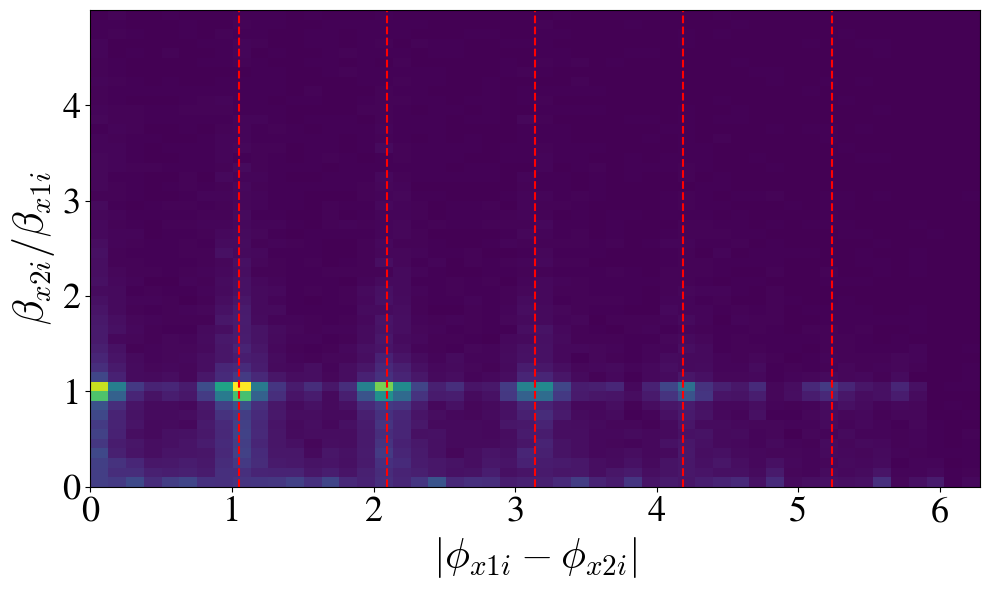
\includegraphics[width=\columnwidth]{chapter4/constrain1.png}
    \caption{2D Histogram of optimum lattice locations where the compensating $K_2$ coefficients with the two new sextupoles are minimized. Red dashed lines correspond to thirds of $\pi$.}
    \label{fig:add2c1}
\end{figure}

\begin{figure}[H]
    \centering
    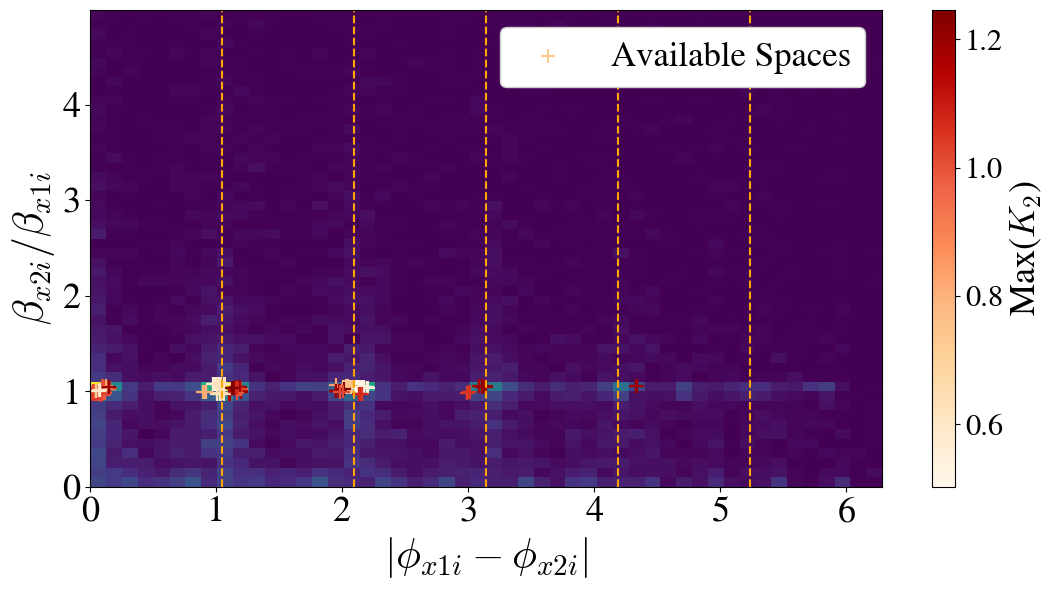
\includegraphics[width=\columnwidth]{chapter4/constrain1_avail.png}
    \caption{2D Histogram of optimum lattice locations where the compensating $K_2$ coefficients with the two new sextupoles are minimized with available drift spaces candidates scattered on top of it.}
    \label{fig:add2c2}
\end{figure}

\begin{figure}[H]
    \centering
    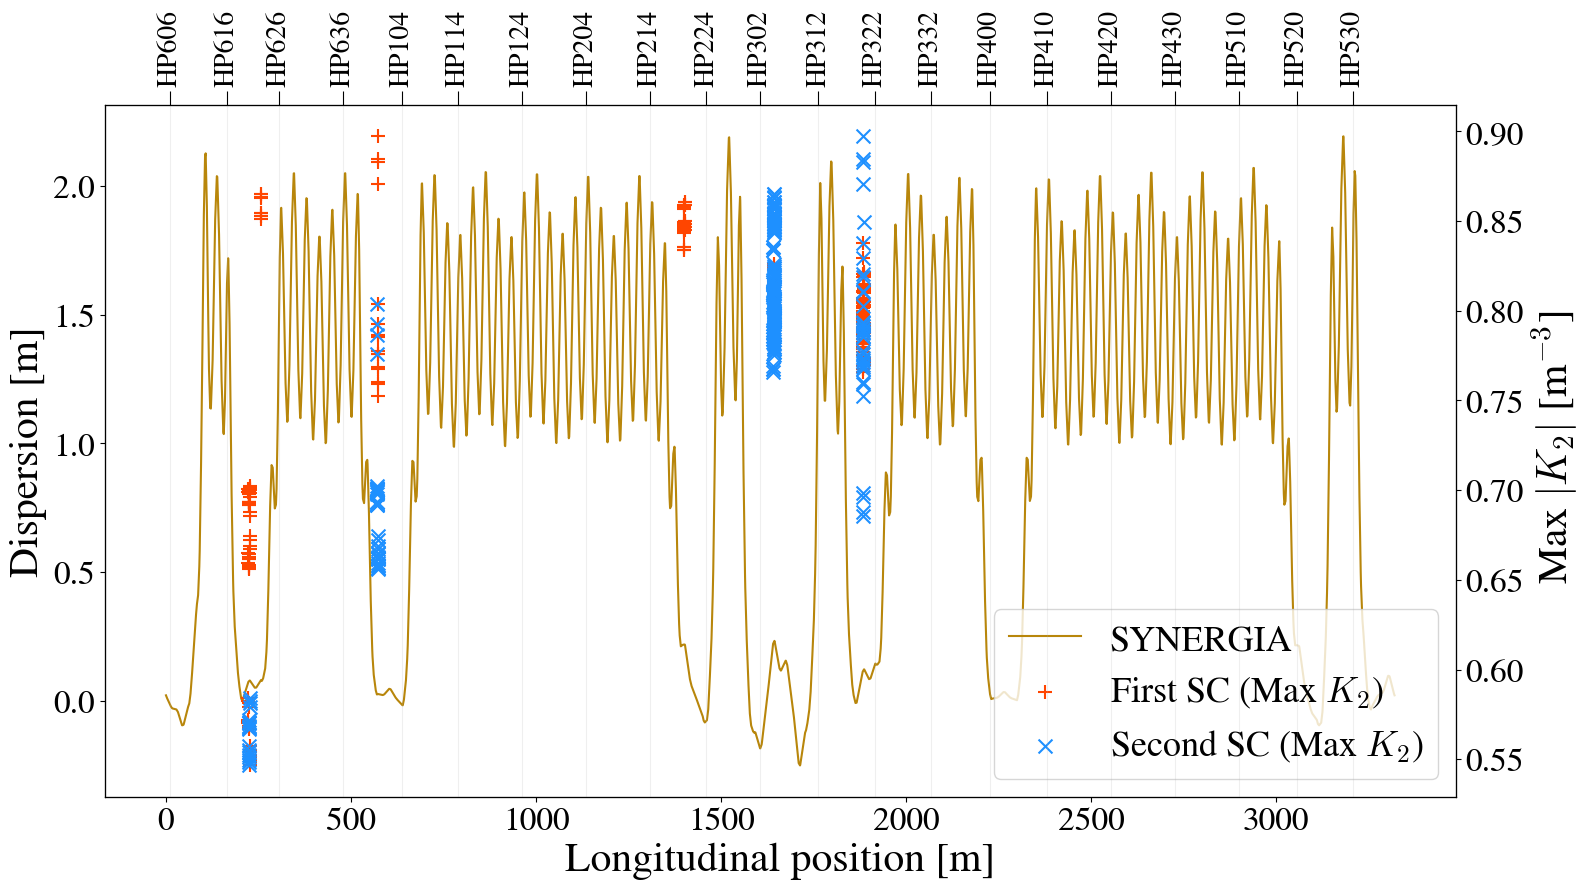
\includegraphics[width=\columnwidth]{chapter4/new_sexts_dx.png}
    \caption{Dispersion function of the Recycler Ring with possible new locations to introduce a pair of sextupole magnets that cancel out $h_{3000}$ and $h_{1020}$ simultaneously. The right y-axis shows the maximum compensation current needed with these new candidates.}
    \label{fig:dxnewsexts}
\end{figure}


\begin{table}[H]
    \centering
    \caption{$K_2$ coefficients that cancel out the $h_{3000}$ and $h_{1020}$ term when the two new 620 sextupoles are introduced. These values were calculated for a Recycler lattice tuned to $Q_x=25.4422$ and $Q_y=24.3915$.}
    \label{tab:k2s620}
    \begin{tabular}{cc}
    \toprule
    \textbf{Sextupole} & $K_2$ [m$^{-3}$] \\ \midrule
     &  \\
    SC220 & -0.263835 \\
     &  \\
    SC222 & 0.463129 \\
     &  \\
    SC319 & 0.480173 \\
     &  \\
    SC321 & -0.407482 \\
     &  \\
    SC620a & 0.581187 \\
     &  \\ 
    SC620b & 0.511139 \\
     &  \\ \bottomrule
    \end{tabular}
    \end{table}

\begin{figure}[H]
    \centering
    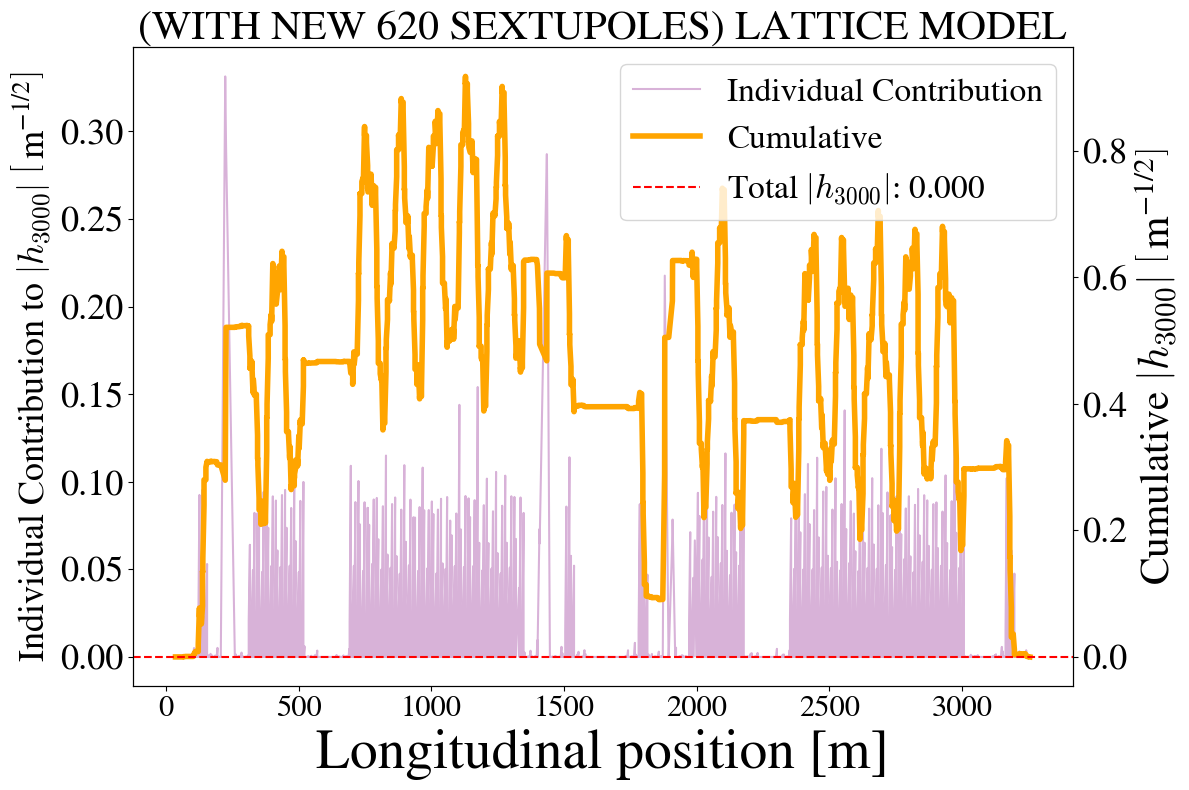
\includegraphics[width=\columnwidth]{chapter4/new_sexts_h3000.png}
    \caption{Distribution of the $h_{3000}$ term around the ring with individual contributions from each relevant element and the cumulative sum from an arbitrary starting point. This is with the new 620 sextupoles powered at the correct currents to cancel out $h_{3000}$ and $h_{1020}$ simultaneously.}
    \label{fig:h3000newsexts}
\end{figure}

\begin{figure}[H]
    \centering
    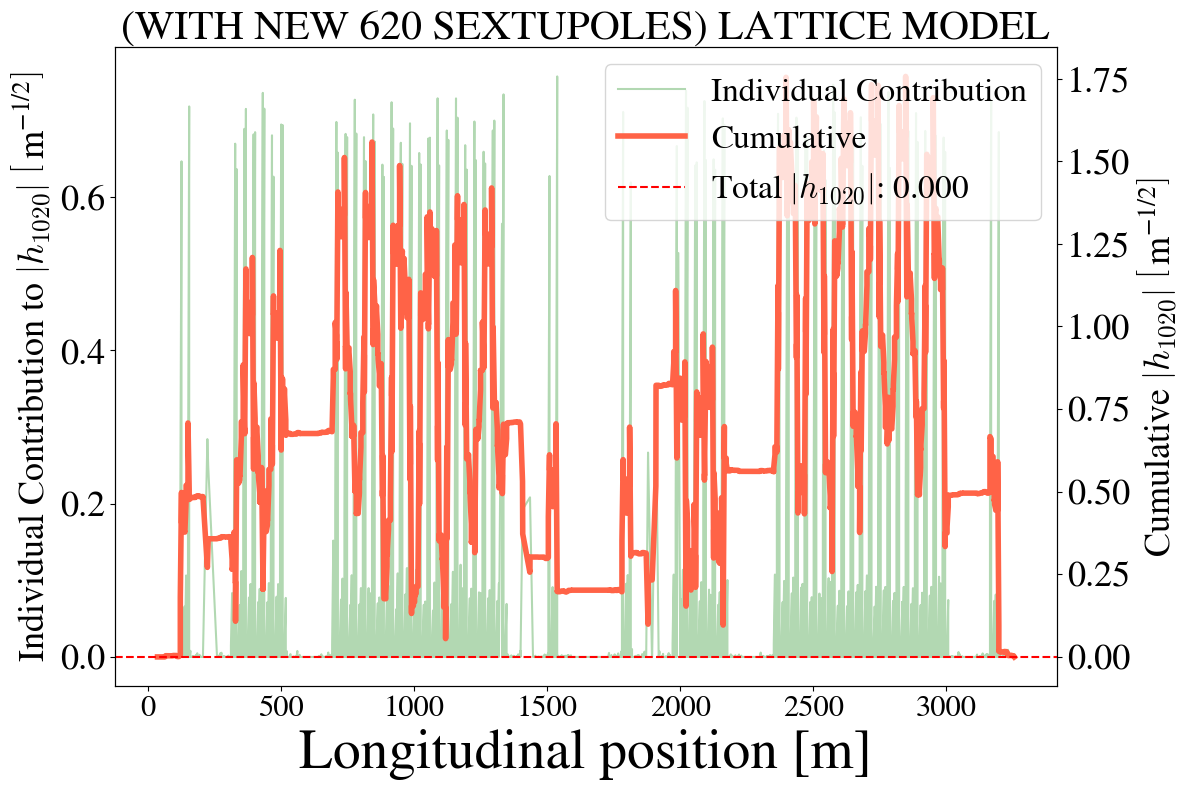
\includegraphics[width=\columnwidth]{chapter4/new_sexts_h1020.png}
    \caption{Distribution of the $h_{1020}$ term around the ring with individual contributions from each relevant element and the cumulative sum from an arbitrary starting point. This is with the new 620 sextupoles powered at the correct currents to cancel out $h_{3000}$ and $h_{1020}$ simultaneously.}
    \label{fig:h1020newsexts}
\end{figure}
